\documentclass[reqno]{amsart}
\usepackage[utf8]{inputenc}
\usepackage[margin=1in]{geometry}
\usepackage[usenames, dvipsnames]{xcolor}
\usepackage{graphicx}
\usepackage{mathtools}
\usepackage{amssymb}
\usepackage{amsthm}
\usepackage{fancyhdr}
\usepackage{adforn}
\usepackage{xparse}
\usepackage{tikz}
\usetikzlibrary{fadings}
%\usetikzlibrary{matrix, positioning, calc}
% Additional math macros that I want in both my notes and my psets
\usepackage[sc, noBBpl]{mathpazo}
\usepackage{mathrsfs}
\usepackage[T1]{fontenc}
\usepackage{calligra}
\usepackage{microtype}
\usepackage[all]{xy}
\usepackage{slashed}
\newcommand{\A}{\mathbb A}
\newcommand{\cat}{\mathsf}
\newcommand{\sC}{\cat C}
\newcommand{\sD}{\cat D}
\newcommand{\sS}{\cat S}
\newcommand{\sA}{\mathscr A}
\newcommand{\sF}{\mathscr F}
\newcommand{\sG}{\mathscr G}
\renewcommand{\P}{\mathbb P}
\newcommand{\cO}{\mathscr O}
\newcommand{\sI}{\mathscr I}
\DeclareMathOperator{\coker}{coker}
\renewcommand{\Im}{\operatorname{Im}}
\newcommand{\pt}{\mathrm{pt}}
\DeclareMathOperator{\Hom}{Hom}
\newcommand{\op}{^{\mathsf{op}}}
\newcommand{\Id}{\mathrm{Id}}
\DeclareMathOperator{\Mat}{Mat}
\newcommand{\m}{\mathfrak m}
%\newcommand{\p}{\mathfrak p}
\newcommand{\q}{\mathfrak q}
\DeclareMathOperator{\MSpec}{MSpec}
\DeclareMathOperator{\Spec}{Spec}
\newcommand{\Top}{\cat{Top}}
\newcommand{\Ring}{\cat{Ring}}
\newcommand{\Mod}{\cat{Mod}}
\DeclareMathOperator{\res}{res}
\newcommand{\Alg}{\cat{Alg}}
\newcommand{\Fun}{\cat{Fun}}
\newcommand{\AffSch}{\cat{AffSch}}
\newcommand{\Ab}{\cat{Ab}}
\DeclareMathOperator{\bl}{--}
\DeclareMathOperator{\Free}{Free}
\DeclareMathOperator{\For}{For}
\newcommand{\Set}{\cat{Set}}
\newcommand{\LocRing}{\cat{LocRing}}
\newcommand{\Grp}{\cat{Grp}}
\newcommand{\Sch}{\cat{Sch}}
\newcommand{\inHom}{\operatorname{\underline{\Hom}}}
\DeclareMathOperator{\Frac}{Frac}
\DeclareMathOperator{\Gal}{Gal}
\DeclareMathOperator{\Nil}{Nil}
\newcommand{\pre}{\sC^{\text{pre}}}
\newcommand{\sh}{_{\text{sh}}}
\newcommand{\G}{\mathbb G}
\DeclareMathOperator{\Proj}{Proj}
\newcommand{\sM}{\mathscr M}
\newcommand{\sV}{\mathscr V}
\newcommand{\fU}{\mathfrak U}
\newcommand{\GL}{\mathrm{GL}}
\DeclareMathOperator{\Sym}{Sym}
% http://tex.stackexchange.com/questions/141434/how-to-type-sheaf-hom
\DeclareMathOperator{\shom}{\mathscr{H}\text{\kern -4pt {\calligra\large om}}\,}
\newcommand{\sL}{\mathscr L}
\DeclareMathOperator{\QC}{QC}
\DeclareMathOperator{\Supp}{Supp}
\newcommand{\sN}{\mathscr N}
\DeclareMathOperator{\Ann}{Ann}
\DeclareMathOperator{\Der}{Der}
\newcommand{\ctcpx}[1]{(#1)^{\text{der}}}
\newcommand{\Dist}{\mathsf{Dist}}
\newcommand{\shdi}{\operatorname{Sh}_{\Dist}}
\DeclareMathOperator{\Sh}{Sh}
\newcommand{\shz}{\mathsf{Sh}_{\text{\rm Zar}}}
\DeclareMathOperator{\Gr}{Gr}
% Source: http://tug.org/pipermail/xy-pic/2001-July/000015.html
\newcommand{\pullbackcorner}[1][dr]{\save*!/#1+1.2pc/#1:(1,-1)@^{|-}\restore}
\newcommand{\pushoutcorner}[1][dr]{\save*!/#1-1.2pc/#1:(-1,1)@^{|-}\restore}
\newcommand{\TDel}{\mathrm{2\Delta}}
\DeclareMathOperator{\Bl}{B\ell}
\newcommand{\cR}{\mathcal R}
\newcommand{\cL}{\mathcal L}
\newcommand{\cH}{\mathcal H}
\newcommand{\refR}{\reflectbox{\(\cR\)}}

\renewcommand{\a}{\alpha}
\renewcommand{\b}{\beta}
%\newcommand{\e}{\epsilon}
\renewcommand{\l}{\lambda}
\renewcommand{\L}{\Lambda}
\newcommand{\g}{\gamma}
\newcommand{\s}{\sigma}
\newcommand{\z}{\zeta}
\newcommand{\RR}{\mathbb{R}}
\newcommand{\NN}{\mathbb{N}}
\newcommand{\QQ}{\mathbb{Q}}
\newcommand{\ZZ}{\mathbb{Z}}
\newcommand{\CC}{\mathbb{C}}
\newcommand{\cC}{\mathcal{C}}
\newcommand{\f}{\frac}
\newcommand{\p}{\partial}
\renewcommand{\P}[3][]{\f{\partial^{#1} #2}{\partial #3 ^{#1}}}
%\newcommand{\avg}[1]{\langle #1 \rangle}
\newcommand{\avg}[1]{\left< #1 \right>}
\newcommand{\?}{\overset{?}{=}}
\newcommand{\Int}{\int_{-\infty}^\infty}
\newcommand{\ket}[1]{\left| #1 \right>} % for Dirac bras
\newcommand{\bra}[1]{\left< #1 \right|} % for Dirac kets
\newcommand{\braket}[2]{\left< #1 \vphantom{#2} \right|
 \left. #2 \vphantom{#1} \right>} % for Dirac brackets
\newcommand{\pv}{\vec{p}}

\newcommand{\grad}[1]{\gv{\nabla} #1} % for gradient
\let\divsymb=\div % rename builtin command \div to \divsymb
\renewcommand{\div}[1]{\gv{\nabla} \cdot #1} % for divergence
\newcommand{\curl}[1]{\gv{\nabla} \times #1} % for curl
\renewcommand{\labelenumi}{(\alph{enumi})}
\let\vaccent=\v % rename builtin command \v{} to \vaccent{}
\renewcommand{\v}[1]{\ensuremath{\mathbf{#1}}}
\newcommand{\uv}[1]{\ensuremath{\mathbf{\hat{#1}}}} % for unit vector
\newcommand{\gv}[1]{\ensuremath{\mbox{\boldmath$ #1 $}}} 
% for vectors of Greek letters
\usepackage{hyperref}
\usepackage{siunitx}

%\usepackage[compat=1.1.0]{tikz-feynman}

% TODO fiddle with colors
\definecolor{newblue}{HTML}{1F98A6}
\definecolor{newred}{HTML}{D95448}
\definecolor{neworange}{HTML}{F29441}
\hypersetup{
	colorlinks,
	linkcolor=newred,
	citecolor=neworange,
	urlcolor=newblue!80!black,
}
\usepackage[all]{hypcap}
\pagestyle{plain}
\setcounter{tocdepth}{1}


\usepackage{titlesec}
\titleformat{\section}[frame]
  {\normalfont}
  {\filright
   \footnotesize
   \enspace Lecture \arabic{section}.\enspace}
  {8pt}
  {\Large\bfseries\filcenter}
\usepackage[dotinlabels]{titletoc}
\titlecontents{section}[1.5em]{}{\contentslabel{2.3em}}{\hspace*{-2.3em}}{\hfill\contentspage}

\renewcommand{\sectionmark}[1]{\markleft\thesection. #1}

\fancyhf{}
\fancyhead[RO,LE]{\small\thepage}
\fancyhead[LO]{\small\slshape\nouppercase{\rightmark}}
\fancyhead[RE]{\small\slshape Advanced Quantum Field Theory Lecture Notes}
\setlength{\headheight}{11.0pt}
\pagestyle{fancy}

\numberwithin{equation}{section}
\newcommand{\orbreak}{
\begin{center}
	\adforn{17}\;\(\cdot\)\;\adforn{18}
	\vspace{0.2cm}
\end{center}
}

\renewcommand{\labelitemi}{\(\circ\)}

% I wanted to allow one to reference parts of a thm/cor/etc. and have it print the thm number too, e.g. 29.2(1),
% but this isn't working right now. Probably the best way to do this would be to play around with enumitem to
% define a new enumerate-like counter and then just use that directly instead of enumerate in comp.

% This feels really wobbly, but so far it's working
\NewDocumentEnvironment{comp}{mm}{%
	\csname #1\endcsname\hfill
	\csname #2\endcsname
}{
	\csname end#2\endcsname
	\csname end#1\endcsname
}

% usage:
% \shortexact[f][g]{A}{B}{C},
%
%			 f    g
% for 0 -> A -> B -> C -> 0,
\DeclareDocumentCommand{\shortexact}{O{} O{} mmmm}{
\xymatrix{
	0\ar[r] & #3\ar[r]^-{#1} & #4\ar[r]^-{#2} & #5\ar[r] & 0#6
}}
% exactly the same, but for 0 -> A -> B -> C
\DeclareDocumentCommand{\leftexact}{O{} O{} mmmm}{
\xymatrix{
	0\ar[r] & #3\ar[r]^-{#1} & #4\ar[r]^-{#2} & #5 #6
}}
% ... and the same, for A -> B -> C -> 0
\DeclareDocumentCommand{\rightexact}{O{} O{} mmmm}{
\xymatrix{
	#3\ar[r]^-{#1} & #4\ar[r]^-{#2} & #5\ar[r] & 0#6
}}



% usage:
% X\dblarrow[r] & Y
%   f
% X => Y
%   g
\DeclareDocumentCommand{\dblarrow}{O{} O{} O{}}{
	\ar@<0.4ex>[#1]^-{#2}\ar@<-0.4ex>[#1]_-{#3}
}
% Note: it would be a useful exercise to figure out how to define this so it can be used as
% \dblarrow[r]^f_g

\everyentry={\displaystyle}

\newcommand{\N}{\mathbb N}
\newcommand{\Z}{\mathbb Z}
\newcommand{\Q}{\mathbb Q}
\newcommand{\R}{\mathbb R}
\newcommand{\C}{\mathbb C}
\newcommand{\F}{\mathbb F}
\newcommand{\vp}{\varphi}
\newcommand{\term}{\emph}
\renewcommand{\vec}[1]{\boldsymbol{\mathbf{#1}}}
\DeclarePairedDelimiter\paren{(}{)}
%\DeclarePairedDelimiter\ang{\langle}{\rangle}
\DeclarePairedDelimiter\abs{\lvert}{\rvert}
\DeclarePairedDelimiter\norm{\lVert}{\rVert}
\DeclarePairedDelimiter\bkt{[}{]}
\DeclarePairedDelimiter\set{\{}{\}}
% Swap paren* and paren, etc., so that the normal version resizes by default.
% Meanwhile, one can use \paren*[\Big]{...} to customize the size easily.
% It would be interesting to wrap this up into a custom \definedelimiter command...
\makeatletter
	\let\oldparen\paren
	\def\paren{\@ifstar{\oldparen}{\oldparen*}}
	\let\oldbkt\bkt
	\def\bkt{\@ifstar{\oldbkt}{\oldbkt*}}
\makeatother
\newcommand{\e}{\varepsilon}
\def\qedsymbol{{\small{\ensuremath{\boxtimes}}}}
\newcommand{\inj}{\hookrightarrow}
\newcommand{\surj}{\twoheadrightarrow}
\DeclareMathOperator{\id}{id}
\newcommand{\ud}{\,\mathrm{d}}
\renewcommand{\d}{\mathrm d}
\newcommand{\dfr}[2]{\frac{\mathrm d #1}{\mathrm d #2}}
\newcommand{\pfr}[2]{\frac{\partial #1}{\partial #2}}

%\catcode`\"=13
%\newcommand{"}[1]{^{(#1)}}
\newtheorem{thm}[equation]{Theorem}
\newtheorem*{thm*}{Theorem}
\newtheorem{lem}[equation]{Lemma}
\newtheorem*{lem*}{Lemma}
\newtheorem{cor}[equation]{Corollary}
\newtheorem{prop}[equation]{Proposition}
\newtheorem{obs}[equation]{Observation}
\theoremstyle{definition}
\newtheorem{ex}[equation]{Exercise}
\newtheorem{exm}[equation]{Example}
\newtheorem{defn}[equation]{Definition}
\newtheorem*{claim}{Claim}
\theoremstyle{remark}
\newtheorem*{rem}{Remark}
\newtheorem*{fct}{Fact}
\newtheorem*{note}{Note}

\begin{document}
\title{General Relativity}
\author{Ian Lim\\ Last updated \today}
\maketitle
{\small\noindent These notes were taken for the \textit{General Relativity} course taught by Malcolm Perry at the University of Cambridge as part of the Mathematical Tripos Part III in Michaelmas Term 2018. I live-\TeX ed them using TeXworks, and as such there may be typos; please send questions, comments, complaints, and corrections to 
\href{mailto:itel2@cam.ac.uk?subject=GR\%20Lecture\%20Notes}{\texttt{itel2@cam.ac.uk}}.\\
Many thanks to Arun Debray for the {\LaTeX} template for these lecture notes: as of the time of writing, you can find him at \url{https://web.ma.utexas.edu/users/a.debray/}.}

\tableofcontents

\section{Friday, October 5, 2018}
	Unlike in previous years, this course is intended to be a stand-alone course on general relativity, building up the mathematical formalism needed to construct the full theory and explore some examples of interesting spacetime metrics. It is linked to the Black Holes course taught in Lent term, which I will also be writing notes for.

Some recommended course materials and readings include the following:
\begin{itemize}
\item Sean Carroll, Spacetime and Geometry
\item Misner, Thorne, and Wheeler, Gravitation
\item Wald, General Relativity
\item Zee, Einstein Gravity in a Nutshell
\item Hawking and Ellis, ``The Large Scale Structure of Spacetime''
\end{itemize}

In Minkowski\footnote{I've heard some USAmericans pronounce this ``min-cow-ski.'' In German, it is ``min-koff-ski.''} spacetime (flat space) we specify points in spacetime by spatial coordinates in $\RR^3$, i.e. the Cartesian coordinates $(x,y,z)$, plus a time coordinate $t$. The line element (spacetime separation) is given by the metric
$$ds^2=-dt^2+dx^2+dy^2+dz^2.$$
$ds$ is the proper distance between $x$ and $x+dx$, $y$ and $y+dy$, $z$ and $z+dz$, and $t$ and $t+dt$. (As is typical in relativity, we work in units where $c=1$. Note that the metric sign convention here is flipped from my QFT notes, which uses the ``mostly minus'' convention-- this is arbitrary and so long as one is consistent it makes no difference.) Using the Einstein summation convention, the metric is usually written more compactly as $$ds^2=\eta_{\alpha\beta}x^\alpha x^\beta,$$ with $\eta_{\alpha\beta}$ the Minkowski space metric.

Let's recall from special relativity that we call separations with $ds^2>0$ ``spacelike,'' with $ds^2<0$ ``timelike,'' and $ds^2=0$ null (or occasionally lightlike).
\begin{defn}
The \term{chronological future} of a point $p$ is the set of all points that can be reached from $p$ along future directed timelike lines, and we call this $I^+(p)$. It is the interior of the future-directed light cone. Conversely we have the chronological past of $p$, $I^-(p)$, which is the interior of the past-directed light cone. We also have the \term{causal future} of $p$, which is the set of all points that can be reached from $p$ along future-directed timelike \emph{or} null lines, and we call this $J^+(p)$. Similarly we have the causal past, $J^-(p)$. Thus $J$ is the closure of $I$ and is the interior \emph{plus} the light cone itself.
\end{defn}

\begin{figure}
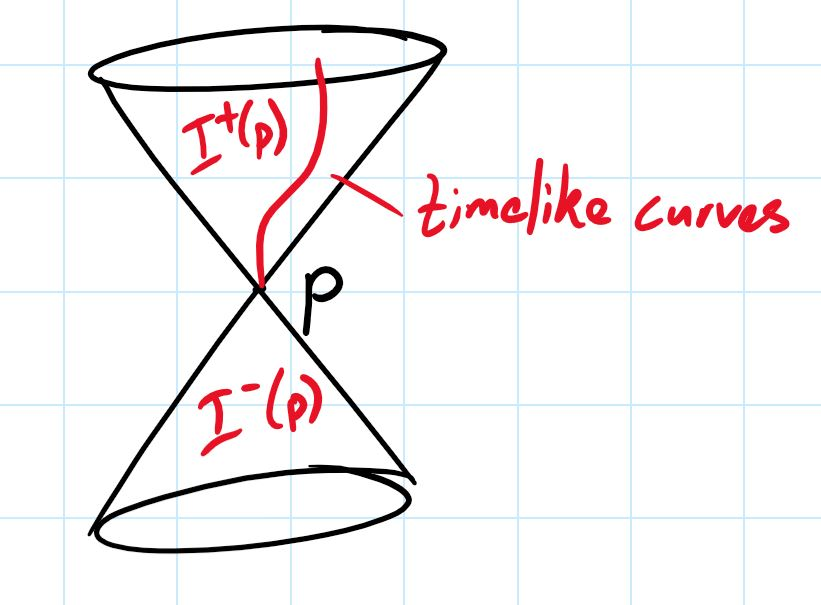
\includegraphics{2018/10/20181005_img1}
\caption{An illustration of the light cones from a point $p$, plus the chronological future $I^+$ and chronological past $I^-$. Also depicted in red is a timelike curve (e.g. a possible particle trajectory in spacetime).}
\end{figure}

Let $x^a(\tau)$ be a curve in spacetime.\footnote{Evidently we are not using the convention that Greek indices range from $0$ to $3$ and Latin indices range from $1$ to $3$. I have copied the lecturer's convention here, but may change to more traditional notation if it becomes relevant.} Then the tangent vector to the curve is $u^a=\frac{dx^a}{d\tau}$. For timelike curves, $u^a u^b \eta_{ab}=-1 \iff \tau$ is the proper time along the curve.
\footnote{The property that $U^\alpha U^\beta \eta_{\alpha\beta}=-1$ is easy to prove. See the Special Relativity catch-up sheet found \href{http://www.maths.cam.ac.uk/sites/www.maths.cam.ac.uk/files/grspecialrelativity.pdf}{here} for some nice exercises in SR: this is exercise 3. Assuming the result of exercise 2 which states that the four-velocity of a massive particle is $U^\mu=\gamma(1,v^i)$, we then have $U\cdot U =\gamma^2(-1+v^2)=\frac{v^2-1}{1-v^2}=-1$. Since this is a fully contracted expression (no indices floating around), it is true in all frames.}
We also know that $\int_p^q d\tau = \Delta \tau$, which just says that the integral of $d\tau$ along a curve from $p$ to $q$ yields the proper time interval, what a clock actually measures.

We also remark that Minkowski space has some very nice symmetries. Since $x,y,$ and $z$ do not appear explicitly in the metric, our spacetime is invariant under translations. It is also invariant under rotations in $\RR^3$. It would be nice to extend rotations to include the time coordinate $t$ as well-- this is exactly what a Lorentz transformation does.

Lorentz transformations in general involve time-- they are defined by the matrices $\Lambda$ which satisfy
$$\Lambda^T \eta \Lambda= \eta,$$
i.e. they preserve the inner product $\eta$ in Minkowski space, forming the group $O(3,1)$. Lorentz transformations consist of rotations in $\RR^3$ and boosts. This is equivalent to the defining property of rotation matrices $R$ that $R^T \delta R=\delta$, meaning that rotation matrices preserve the standard Euclidean inner product in $\RR^3$ and form the group $O(3)$.\footnote{Strictly, $O(3)$ also includes reflections-- for matrices which preserve both orientation and the inner product, we must also require that $\det R=+1$, defining the group $SO(3)$. We'll see a similar caveat with the Lorentz group in just a second.}
Written explicitly, the Lorentz boost in the $x$-direction to a frame moving with velocity $v$ is
\begin{eqnarray*}
t\to t'&=&\frac{t-vx}{\sqrt{1-v^2}}\\
x\to x'&=&\frac{x-vt}{\sqrt{1-v^2}}\\
y\to y'&=&y\\
z\to z'&=&z
\end{eqnarray*}
We may also write it in matrix notation,
$${\Lambda^a}_b =
\begin{pmatrix}
\gamma&-\gamma v &0 & 0\\
-\gamma v & \gamma & 0 & 0\\
0&0&1&0\\
0&0&0&1
\end{pmatrix}$$
where $\gamma$ is defined in the usual way by $\gamma \equiv \frac{1}{\sqrt{1-v^2}}$.

Rather than constructing the (in general complicated) Lorentz boost in an arbitrary direction, it is often more convenient to rotate one's frame of reference in $\RR^3$ so the boost is in the new $x$-direction, perform the Lorentz boost, and then transform back:
$$R^T \Lambda R= \Lambda_R,$$
where $\Lambda_R$ is a new Lorentz transformation.\footnote{It's easy to check that $\Lambda_R$ really is a Lorentz transformation-- just observe that rotations alone are a subset of Lorentz transformations, since they preserve the inner product on $\RR^3$ and do not affect the time coordinate. In the language of group theory, rotations form an $SO(3)$ subgroup of the full Lorentz group $O(3,1)$-- see Definition \ref{lorentzgroup}. Therefore any combination of rotations and Lorentz boosts will form another valid Lorentz transformation by the group closure property.}

\begin{defn}\label{lorentzgroup}
The Lorentz transformations taken together form the \term{Lorentz group}. It satisfies the group axioms of identity, unique inverses (since $\det\Lambda \neq 0$), associativity (from associativity of matrix multiplication), and closure (see footnote for proof).\footnote{More precisely, we know that the determinant is nonzero since $-1=\det{\eta}=\det(\Lambda^T\eta\Lambda)=\det(\Lambda^T)\det(\eta)\det(\Lambda)=(-1)\det(\Lambda)^2\implies \det(\Lambda)=\pm 1 \neq 0$. To prove closure, suppose $\Lambda_1,\Lambda_2$ are Lorentz transformations. The product $\Lambda_1\Lambda_2$ then satisfies $(\Lambda_1\Lambda_2)^T \eta(\Lambda_1\Lambda_2)= \Lambda_2^T \Lambda_1^T \eta\Lambda_1 \Lambda_2 = \Lambda_2^T \eta \Lambda_2 = \eta$, so $\Lambda_1\Lambda_2$ is also a Lorentz transformation.}
\end{defn}

$\Lambda$ can include reflections in time or space. To avoid such complications, we sometimes refer to the \term{proper orthochronous Lorentz group,} i.e. to exclude space and time reversals, but often we are more careless and simply call it the Lorentz group.
\begin{defn}
The \term{Poincar\'e group} is then the semidirect product of Lorentz transformations and translations. This is the group of symmetries of Minkowski space.
\end{defn}
We have translations defined as
$$x^a\to {x^a}'=x^a+\Delta x^a$$
and also Lorentz transformations, with the property
$${(\Lambda^T)_a}^c \eta_{cd} {\Lambda^d}_b=\eta_{ab}.$$


\begin{defn}
We also have \term{contravariant vectors} (indices up) written $u^a$ and their corresponding \term{covariant} vectors (indices down) $$u_a\equiv\eta_{ab}u^b,$$ where we have used the metric to lower an index. These are sometimes equivalently called simply vectors and covectors. We can also raise indices using the inverse metric $\eta^{ab}$ (defined by $\eta^{ab}\eta_{bc}=\delta^a_c$). Thus
$$u^b=\eta^{ba}u_a.$$
\end{defn}

We define the Lorentz transformation of a contravariant vector as
$u^a\to {u^a}' = {\Lambda^a}_b u^b.$  For instance, $x^a$ is an example of a contravariant vector.

\begin{defn}
A \term{scalar} is an object which is invariant under a Lorentz transformation. We saw that a covariant vector transforms with right multiplication by the Lorentz transformation, whereas a contravariant vector transforms by left multiplication. 

More generally, a \term{tensor of type $(r,s)$} transforms with $r$ copies of the Lorentz transformation on the $r$ up indices and $s$ copies of the Lorentz transformation on the $s$ down indices, 
\begin{equation}
{T^{\mu_1 \mu_2\ldots \mu_r}}_{\nu_1 \nu_2 \ldots \nu_s} \to {T^{\alpha_1 \alpha_2\ldots \alpha_r}}_{\beta_1 \beta_2 \ldots \beta_s}=\Lambda^{\alpha_1}_{\mu_1} \ldots \Lambda^{\alpha_r}_{\mu_r} {T^{\mu_1 \mu_2\ldots \mu_r}}_{\nu_1 \nu_2 \ldots \nu_s} \Lambda^{\nu_1}_{\beta_1}\ldots \Lambda^{\nu_s}_{\beta_s}
\end{equation}

By this definition, a scalar may be thought of as a type $(0,0)$ tensor, a contravariant vector a type $(1,0)$ tensor, and a covariant vector a type $(0,1)$ tensor.
\end{defn}

\section{Monday, October 8, 2018}
	Today, we'll start by remarking that Maxwell's equations can be written compactly in 4-vector format. Recall from a good course on electrodynamics that we define the electromagnetic field strength tensor $F^{\mu\nu}$ as
$$F^{\mu\nu}=\begin{pmatrix}
0& E_x & E_y & E_z\\
-E_x & 0 & B_z & - B_y\\
-E_y & -B_z & 0 & B_x\\
-E_z & B_y & -B_x & 0
\end{pmatrix}.$$
$F^{\mu\nu}$ is a totally antisymmetric rank two tensor. Defining the four-current $j^\mu \equiv(\rho, \vec{j})$ with $\vec{j}$ the ordinary current density and $\rho$ the charge density, we see that
$$\p_a F_{bc} +\p_b F_{ca} +\p_c F_{ab}=0$$
and
$$\p_a F^{ab}=-j^b.$$

But there's something strange about this-- these equations in their current form hold for Cartesian coordinates only. Of course, the laws of physics (as expressed through empirical results in experiments) cannot depend on the coordinate system we use to define them. 
\begin{exm}
The Minkowski metric takes the Cartesian form
$$ds^2=-dt^2+dx^2+dy^2+dz^2$$
but if we pass to spherical coordinates, the metric now takes the form 
$$ds^2=-dt^2+dr^2+r^2d\theta^2 +r^2 \sin^2 \theta d\phi^2=g_{ab}dx^a dx^b,$$
where $x^a=(t,r,\theta,\phi).$
\end{exm}

General relativity is thus motivated by a desire to understand how the laws of physics are invariant not just under Lorentz transformations but general coordinate transformations. It is also motivated by the \term{weak equivalence principle}, which states that inertial mass and gravitational mass are the same thing-- the $m$ in $F=ma$ and the $m$ in $F=-\frac{GMm }{r^2}$ are the same mass! This is closely related to the \term{Einstein equivalence principle}, which states that in a freely falling frame, the laws of physics are those of special relativity. One cannot distinguish between being in freefall under a gravitational field and simply being at rest in no gravitational field.

We consider spacetime to be a 4-dimensional system ($3+1$ dimensions, if you like) and in particular it has a manifold structure. We may make an explicit choice of some coordinates $\set{x^a}$ that label points in (a coordinate patch of) $M$, but it would be nice to define vectors in a way that is independent of the coordinates. This will lead us to revisit vectors and covectors.

Consider a parametrized curve $\lambda(\tau):\RR\to M$ sitting in $M$. Now take $f=f(x^a)$ to be a differentiable function of the coordinates, and define an operator that maps $f$ into the total derivative $df/dt$: by applying the chain rule, we have
$$\frac{df}{dt}=\P{x^a}{t}\left(\P{}{x^a}f\right).$$
Thus a vector $V$ is a linear differential operator that acts on $f$: explicitly, we can write $$V=\P{x^a}{t}\P{}{x^a},$$ where the $\P{x^a}{t}$ are called the components of the vector and denoted by $V^a$. The right way to think of a vector is as a coordinate-independent generalization of a directional derivative. The components will in general transform when we change coordinates, but the vector as an operator stays the same.

That said, a general vector can be written in its components in some coordinate basis $x^a$ as
$$V= V^a \P{}{x^a}.$$

Thinking back to our curve $\lambda(\tau)$, we may expand our coordinates locally as $x^a(\tau)=x^a (\tau_0)+V^a (\tau-\tau_0)+O((\tau-\tau_0)^2)$, where $V$ is the tangent vector to some curve through the point $\tau_0$. (Okay, we're being a bit careless with notation here-- the instructor has written $\lambda(t)$, but sometimes $t$ is a coordinate on the manifold.) Therefore we may also interpret (tangent) vectors as describing how our manifold curves locally about a point.

Vectors (as the name suggests) form a vector space.\footnote{We get most of the vector space axioms for free. Commutativity and associativity follow from doing component-wise addition in a basis, as does distributivity of scalar sums. The additive identity is the vector where all components are zero. The additive inverse for a vector with components $V^a$ is just $-V^a$. The scalar multiplication identity is automatic.} 
If $W, Y$ are vectors, $\alpha,\beta$ real numbers, then $\alpha W + \beta Y$ is another vector with components
$$(\alpha W^a+\beta Y^a)\P{}{x^a}.$$

As linear differential operators, vectors also obey the Leibniz rule
$$V^a \P{}{x^a}(fg)= V^a \P{f}{x^a} g+ f V^a \P{g}{x^a}.$$

The space of tangent vectors at a point $p$ is called $T_p(M)$. Recall that we defined our tangent vectors with respect to its components in some basis $x^a$. But if we now change to some new coordinates $\tilde x^b = \tilde x^b(x^a)$, then by the chain rule our basis vectors $\P{}{x^a}$ transform as
$$\P{}{x^a}=\P{\tilde x^{b}}{x^a}\frac{\partial}{\partial \tilde x^b}.$$
But $V$ as an operator is invariant-- it does not depend on our choice of coordinates, so its components must also change. If we rewrite $V$ in a different set of coordinates, we find that
$$V=V^a \P{}{x^a} = V^a \P{\tilde x^b}{x^a}\frac{\p}{\p\tilde x^b}$$
by the chain rule. Since $V$ is independent of basis,
$$V=V^a \P{}{x^a}= \tilde V^a \P{}{\tilde x^a},$$ so by comparison we see that the components of $V$ transform as
$$V^a\to \tilde V^{a'} = \frac{\p\tilde x^{a'}}{\p x^a} V^a.$$
In other words, tangent vectors transform as contravariant vectors, which we recognize as a generalization of the formula in special relativity where we had $$\P{\tilde x^{a'}}{x^a}=\Lambda^{a'}_{a}$$
with $\Lambda^{a'}_{a}$ the Lorentz transformation.

\begin{defn}
We may also define \term{one-forms}, which are covariant vectors at some point $p$. Thus the inner product $\langle \omega, V\rangle$ is a real number, with $\omega$ a 1-form and $V$ a vector. The inner product is bilinear:
if $V=\alpha Y + \beta W,$ then
$$\langle \omega, \alpha Y + \beta W\rangle = \alpha\langle \omega, Y\rangle +\beta \langle \omega, W\rangle$$
and similarly for the first argument, if $\omega = \alpha \eta+\beta \xi$
$$\ang{\alpha \eta +\beta\xi, V} = \alpha \ang{\eta, V} +\beta \ang{\xi, V}.$$
\end{defn}

Let us write $V$ in a basis, $V=V^a E_a$ with $E_a$ some set of basis vectors. Then $\omega= \omega_a E^a$ has components in some basis of one forms $E^a$. We have that $\ang{E^a, E_b}=\delta^a_b$, where $E^a$ forms a basis of 1-forms which is dual to the ordinary basis vectors. It is often convenient to take the basis for the tangent space to be $\p/\p x^a$ and the basis for the dual (i.e. the cotangent space) to be $dx^a$. (Remark: the components $V^a$ of a vector transform like coordinate functions, while the components of a one-form $\omega_a$ transform like basis vectors $E_a$.) We can then compute the inner product of a generic one-form and a vector, %As the components of a 1-form are real numbers (and the same is true of vectors) we may compute
\begin{eqnarray*}
\ang{\omega,V}&=&\ang{\omega_a E^a, V^b E_b}\\
&=& \omega_a V^b \delta^a_b\\
&=& \omega_a V^a.
\end{eqnarray*}

\section{Wednesday, October 10, 2018}
	\subsection*{A quick admin note} There is no lecture Monday 15 October. In addition, office hours will be Tuesdays at 4 PM in B1.26. Moving on.

Let us recall that we have a multiplication law on one-forms and vectors, 
$$\langle \omega, X\rangle = \omega_a X^a$$
for $\omega$ any one-form, $X$ any vector. That is, we can write this product in terms of the components of $\omega$ and $X$. 

\begin{defn}
With this in mind, we define the \term{differential} of a function $f:M\to \RR$ to be the one-form $df$, such that
$$\langle df, X \rangle = Xf$$
(that is, $X$ as a differential operator acting on $f$).
\end{defn}
\begin{exm}
Non-lectured example: consider the function $f=x+y$ in $\RR^3$ and let $X= \P{}{y}$. (We have chosen a coordinate basis to make the computation clearer.) Then $df=dx+dy$ (a one-form) and now
$$\langle df, X \rangle = Xf = \P{}{y}(x+y)=1.$$
\end{exm}

Recall we have a basis of 1-forms $E^a$ and a basis of vectors $E_b$ with $\langle E^a, E_b \rangle = \delta^a_b$. In a coordinate basis, the basis vectors take the form
$$E_a = \P{}{x^a}\text{ and }E^b= dx^b.$$
Thus
$$\langle dx^a, \P{}{{x^b}}\rangle = \delta^a_b.$$
\begin{defn}
A one-form is \term{exact} if it can be written as $df$ for some scalar $f$. For instance, $dt$ and $dr$ are exact because they are the differentials of $t$ and $r$, but $rd\theta$ is not exact. However, the one-form $r dr$ is exact, since it can be written $d(r^2 /2).$
\end{defn}
In Minkowski space with Cartesian coordinates, the natural basis of one-forms $dt,dx,dy,dz$ forms a coordinate basis since each of these is exact, and the basis of vectors dual to this is $\P{}{t},\P{}{x},\P{}{y},\P{}{z}$. 

However, in spherical coordinates the Minkowski metric looks different. It takes the form
$$ds^2=-dt^2 +dr^2+r^2d\theta^2 +r^2 \sin^2\theta d\phi^2.$$
The basis of one-forms here, 
$$dt, dr, rd\theta, r\sin\theta d\phi$$
is not a coordinate basis because these are not all of the form $df$.
The set of basis vectors dual to the one-forms in spherical coordinates is also kind of bad. They take the form 
$$\P{}{t},\P{}{r},\frac{1}{r}\P{}{\theta},\frac{1}{r\sin\theta}\P{}{\phi},$$ and these are not a coordinate basis because they are not of the form $\P{}{{x^a}}$ (equivalently, they are not dual to exact one-forms).

However, we remark that our defining equation for the product of a one-form and vector produces an ordinary scalar, which must be invariant under coordinate transformations:
$$\langle \omega, X\rangle = \omega_a X^a\text{ in any basis.}$$
This determines how the components of a one-form $\omega_a$ change under coordinate transformations.
In a coordinate basis, we know that the components of a vector transform like coordinate functions:
$$X^a\to \tilde X^{a'}=\frac{\p \tilde x^{a'}}{\p x^a} X^a.$$
Therefore in a coordinate basis, the components of a one-form must transform in the inverse way,
$$\omega_a \to \tilde \omega_{a'} = \frac{\p x^a}{\p \tilde x^{a'}} \omega_a.$$
Note where the primed indices lie and which coordinates are the new coordinates $\tilde x$ versus the old coordinates $x$. A little mnemonic-- to keep the indices straight, just remember that primed indices go with $\tilde x$ coordinates, and we can only contract over pairs of up and down indices. In particular, when $x^a$ is in the denominator\footnote{Okay, technically not the denominator since it's a derivative but you know what I mean.} of a derivative $\P{\tilde x^{a'}}{x^a}$ it acts like an index-down quantity, so it should contract with an index-up object, namely the vector components $X^a$. Similarly, when $x^a$ is in the numerator of the derivative it remains index-up and should therefore contract with the index-down one-form components.%The factor here $\frac{\p x^a}{\p \tilde x^{a'}}$ is analogous to how the Lorentz transformation acts (as the Lorentz transformation is a particular coordinate transformation satisfying certain constraints).

Suppose that $\langle df ,X\rangle = 0$ for some $df$ and $X$ an arbitrary vector. If we are working in $n$ dimensions, this equation gives one constraint on the $n$ components of $X$. Thus, there are still $(n-1)$ different linearly independent choices of $X$ which solve this equation, so the solutions $X$ therefore span an $n-1$-dimensional space. We have put one constraint specified by $f$ on our space of all possible $X$ such that $df$ is the normal to the surface $f=$ constant.

\begin{exm}
Again, a non-lectured concrete example. Let us again work in $\RR^3$ and set $f=x.$ Then a general $X$ can be written as $X^a \P{}{x^a}$ and the condition that $\ang{df,X}=0$ can be computed explicitly as
$$\ang{df,X}=\paren{X^1 \P{}{x}+X^2 \P{}{y}+X^3 \P{}{z}}(x)=X^1(1)=0.$$
Therefore our surface is defined by $X^1=0$ but we may choose $X^2$ and $X^3$ freely (one constraint gives $3-1=2$ free choices). Indeed, we see that $df=dx$ is normal to the surface $f=x=$ constant.
\end{exm}

\begin{defn}
A \term{tensor} is a coordinate-invariant object which generalizes the idea of vectors and covectors. Written in terms of basis one-forms $E^a$ and basis vectors $E_a$, a tensor of type $(r,s)$ takes the form
$$T={T^{a_1\ldots a_r}}_{b_1\ldots b_s} E_{a_1}\otimes E_{a_2}\otimes\ldots \otimes E_{a_r} \otimes E^{b_a}\otimes \ldots \otimes E^{b_s},$$
where $\otimes$ is the tensor product (not just a direct product!).\footnote{Tensor products are more complicated than direct products because their addition structure is multilinear, i.e. linear in each argument individually but not all simultaneously. Where it might make sense to add $(2,1)+(1,2)=(3,3)$ in $\RR\times \RR$, the equivalent tensor product in $\RR \otimes \RR$ would have $2 \otimes 1 + 1\otimes 2 = 2\otimes 1 + 2 \otimes 1= (2+2)\otimes 1 = 4 \otimes 1$. So this is quite a different beast. More info on tensor products and tensors as mathematical constructions can be found at \url{https://jeremykun.com/2014/01/17/how-to-conquer-tensorphobia/}.}
\end{defn}

The tensor $T$ (not the components!) is coordinate invariant, so in a coordinate basis the components of $T$ transform as
$${{\tilde T}^{a_1'\ldots a_r'}}_{b_1'\ldots b_s'}=\frac{\p \tilde x^{a_1'}}{\p x^{a_1}} \ldots \frac{\p \tilde x^{a_r'}}{\p x^{a_r}} \frac{\p x^{b_1}}{\tilde x^{b_1'}} \ldots \frac{\p x^{b_s}}{\tilde x^{b_s'}} {T^{a_1\ldots a_n}}_{b_1\ldots b_s}.$$
In a non-coordinate basis, these $\frac{\p \tilde x^{a'}}{\p x^a}$ are replaced by some general functions $\Phi ^{a'}_a$ where $\tilde x^{a'}=\Phi^{a'}_a x^a$.

We can perform the symmetrization operation, denoted by putting indices to be symmetrized in parentheses:
$$X_{(a_1 \ldots a_r)}\equiv \frac{1}{r!}\left[\text{sum of all permutations of }a_1\ldots a_r\right].$$
For example, $X_{(ab)}=\frac{1}{2}\left[X_{ab}+X_{ba}\right]$. Here, the factorial accounts for that the symmetrization of an already-symmetric tensor should just be that tensor (so that if $X_{ab}=X_{ba},X_{(ab)}=\frac{1}{2}[X_{ab}+X_{ba}]=X_{ab}$). 

Similarly we have the antisymmetrization operation, denoted by putting indices to be antisymmetrized in square brackets:
$$X_{[a_1\ldots a_r]}=\frac{1}{r!}\left[\text{sum over all even permutations } - \text { sum of all odd permutations}\right].$$
For example, $X_{[ab]}=\frac{1}{2}[X_{ab}-X_{ba}].$ Having defined symmetrization and antisymmetrization, we now consider a special class of tensor-- the totally antisymmetric $(0,p)$ tensor.

\begin{defn}
A \term{differential $p$-form} is a tensor of type $(0,p)$ which is antisymmetric on all indices, i.e. $A_{a_1\ldots a_p}=A_{[a_1 \ldots a_p]}$. Some familiar $p$-forms include the $2$-form $F_{\mu\nu}$ from electromagnetism and the Levi-Civita symbol $\epsilon_{ijk}$.
\end{defn}
We can describe $A$ in terms of basis vectors $E^a$ using a construction called the wedge product.
\begin{defn}
The \term{wedge product} is a special kind of antisymmetrizing multiplication of a $p$-form and a $q$-form. For a $p$-form $A=A_{a_1\ldots a_p}$ and a $q$-form $B=B_{b_1\ldots b_q}$, the wedge product $A\wedge B$ is given by
$$(A\wedge B)_{a_1\ldots a_p b_1 \ldots b_q}\equiv A_{[a_1\ldots a_p}B_{b_1\ldots b_q]}.$$
For instance $A\wedge B = (-1)^{pq}B \wedge A$ (this is easy to prove-- we simply switch the $q$ indices of $B$ past the $p$ indices of $A$ and pick up the appropriate $pq$ sign flips along the way).
\end{defn}
As an invariant object, the $p$-form $A$ can be written as $$A=A_{a_1\ldots a_p} E^{a_1}\wedge \ldots \wedge E^{a_p},$$ where $A_{a_1\ldots a_p}$ are now the components of the $p$-form $A$.

\begin{defn}
We also define the exterior derivative, a generalization of the usual derivative $\p_\mu$:
$$(dA)_{ba_1 \ldots a_p} \equiv \P{}{{x^{[b}}} A_{a_1 \ldots a_p]}=\p_{[b}A_{a_1 \ldots a_p]}$$
defines a $p+1$-form, as it is by definition antisymmetric in its $p+1$ indices.
The exterior derivative of a product follows a variation of the Leibniz rule:
$$d(A\wedge B)=dA\wedge B +(-1)^p A\wedge dB.$$
Note that $ddA=0$, so $d$ is nilpotent (it kills all exact differentials).\footnote{Suppose we compute $ddA$: then we will have two derivatives in our expression $\p_{[\mu} \p_\nu A_{a_1\ldots a_p]}$. But derivatives commute, so to every $\p_\alpha \p_\beta$ term in the antisymmetrization sum there will be a corresponding $-\p_\beta \p_\alpha$ term. These terms cancel no matter what $A$ is, so $ddA=0$ identically.}
\end{defn}

The gradient is a simple example of an exterior derivative of a 0-form (AKA a scalar):
$$(d\phi)_\mu=\p_\mu \phi.$$

We now introduce the metric, a very special rank two (i.e. two-index) symmetric tensor usually denoted $g_{\mu\nu}$.\footnote{So far, we have been using Latin indices everywhere. In most GR contexts, Greek indices $\mu,\nu,\sigma,$ etc. are used to range over $0,1,2,3$ and Latin indices $i,j,k$ over $1,2,3$ (the spatial components). Here, we follow the lecturer's convention of using Latin $a,b,c,d$ for all indices but note that it is nonstandard.} The metric generalizes the idea of distance from Euclidean geometry to curved spaces. Unlike the Euclidean metric, the scalar which the metric spits out is not guaranteed to be non-negative-- recall from special relativity that a timelike four-vector $V^\mu$ has a ''length'' given by $\eta_{\mu\nu} V^\mu V^\nu <0$. However, it is a scalar invariant and therefore preserved under arbitrary coordinate transformations.

From prior experience with special (or general) relativity, we might have an intuition that the metric also has something to do with gravitation. The line element $ds$ (defined by $ds^2 = g_{ab}dx^a dx^b$) is invariant and is therefore a (symmetric) tensor. In a freely falling frame, the metric of Minkowski space is $$\tilde \eta_{a'b'} = \frac{\p x^a}{\p\tilde x^{a'}}\frac{\p x^b}{\p \tilde x^{b'} }g_{ab}.$$ Do such $\frac{\p x^a}{\p\tilde x^{a'}}$ always exist? The answer turns out to be yes-- $g_{ab}$ is not degenerate, so one may diagonalize it and then rescale the eigenvalues. Sylvester's theorem states that if $g$ has $r$ positive eigenvalues, $s$ negative eigenvalues, then diagonalizing preserves this.%it's super unclear how this all applies, TBH. 

Therefore given a metric $g_{ab}$ that is non-degenerate, the inverse metric $g^{ab}$ can be defined such that $g^{ab}g_{bc}=\delta^a_c$ the Kronecker delta. One may then use the metric and the inverse metric to raise and lower indices:
$V_b=g_{bc}V^c$ and $V^a = g^{ab}V_b$.

\textit{``There are more unknowns than there are knowns.''} A brief summary of this course.

\section{Friday, October 12, 2018}
	Previously, we defined the exterior derivative, which took a $p$-form to a $p+1$-form. Now we will define the covariant derivative, an operation which in general takes a tensor of type $(r,s)$ to a tensor of type $(r,s+1)$.

Suppose we start with a scalar field $\phi(x)$. The ordinary derivative is just
$$\p_a \phi=\P{\phi}{{x^a}}.$$
Let us change coordinates to ${\tilde x^{a'}}$ some function of the original coordinates. Then this derivative transforms as
$$\p_{a'}\phi= \frac{\p x^a}{\p {\tilde x}^{a'}} \P{}{x^a}\phi = \frac{\p x^a}{\p {\tilde x}^{a'}}\p_a \phi.$$
That is, it transforms in the way we expect an index-down quantity to transform, with the correct factor of $\frac{\p x^a}{\p {\tilde x}^{a'}}.$
We might ask whether the partial derivative of a vector transforms in the same way. The answer is no-- instead, we get something a little different.

\begin{align*}
\p_{b} V^{a}\to \p_{b'} \tilde V^{a'} &= \left(\frac{\p x^b}{\p \tilde x^{b'}} \P{}{x^b}\right) \left( \frac{ \p \tilde x^{a'}}{\p x^a} V^a\right)\\
&=\frac{\p x^b}{\p \tilde x^{b'}} \frac{\p \tilde x^{a'}}{\p x^a} \p_b V^a+ \frac{\p x^b}{\p \tilde x^{b'}}\frac{\p^2 \tilde x^{a'}}{\p x^a \p x^b}V^a.
\end{align*}
This first part is tensorial, but the second part is not (it has a term which is a second derivative of the coordinates). In order to get a tensor, we must add a correction term to the partial derivative. 
\begin{defn}
This motivates us to define the \term{covariant derivative} by
$$\nabla_b V^a \equiv \p_b V^a +\Gamma^a_{bc} V^c$$
where $\Gamma^a_{bc}$ is called a \term{connection}. As the name suggests, a covariant derivative is a derivative which transforms in a tensorial way under arbitrary coordinate transformations.
\end{defn}
We can figure out how $\Gamma$ transforms under coordinate transformations:
$$\tilde \Gamma^{a'}_{b'c'}=\frac{\p \tilde x^{a'}}{\p x^a} \frac{ \p x^b}{\p \tilde x^{b'}}\frac{\p x^c}{\p \tilde x^{c'}} \Gamma^a_{bc}-\frac{\p^2 \tilde x^{a'}}{\p x^b \p x^c}\frac{\p x^b}{\p \tilde x^{b'}}\frac{\p x^c}{\p\tilde x^{c'}}.$$
So $\Gamma$ does \emph{not} transform as a tensor, but that's actually what we want-- this correction term allows us to get a proper tensor when we take the covariant derivative of a vector. Thus
$$\nabla_b V^a \to \nabla_{b'}V^{a'}=\frac{\p x^b}{\p \tilde x^{b'}} \frac{\p \tilde x^{a'}}{\p x^a}\p_b V^a+\frac{\p \tilde x^{a'}}{\p x^a} \frac{ \p x^b}{\p \tilde x^{b'}} \Gamma^a_{bc} V^c.$$
so $\nabla_b V^a$ is an honest tensor. We'd also like $\nabla$ to be linear and obey the Leibniz rule: for two tensors $T,S$ and two real numbers $\alpha,\beta\in \RR$, we should have
$$\nabla(\alpha T+\beta S)= \alpha \nabla T+\beta \nabla S$$
and also
$$\nabla(T\otimes S)=\nabla T \otimes S + T\otimes \nabla S.$$

For a vector $V$ and a one-form $W$, define the scalar $S=V^a W_a$. Then
\begin{align*}
\nabla_a S&= \p_a S\\
&= (\p_a V^b)W_b+ V^b(\p_a W_b)\\
&= (\nabla_a V^b)W_b- \Gamma^b_{ac} V^c W_b+V^b(\p_a W_b)\\
&= (\nabla_a V^b)W_b+ V^b \nabla_a W_b.
\end{align*}
Therefore for the Leibniz rule to hold on the product of a vector and a one-form, it must be that
$$\nabla_b W_a \equiv \p_b W_a - \Gamma^c_{ba}W_c.$$
Note the sign flip from the vector definition! More generally, we can use Leibniz to deduce what the covariant derivative operator is on a general tensor of type $(r,s)$.
$$\nabla_c T^{a_1\ldots a_r}_{b_1\ldots b_s} = \p_c T^{a_1\ldots a_r}_{b_1\ldots b_s}+ 
\Gamma^{a_1}_{cd} T^{da_2 \ldots a_r}+\Gamma^{a_2}_{cd} T^{a_1 d a_3 \ldots a_r}_{b_1\ldots}+\ldots + \Gamma^{a_r}_{cd}T^{a_1a_2\ldots d}_{\ldots} - \Gamma^d_{cb_1}T^{\ldots}_{db_2 \ldots b_s}- \Gamma^d_{cb_2} T^{\ldots}_{b_1 d \ldots b_s}-\ldots - \Gamma^d_{cb_s} T^{\ldots}_{b_1 b_2 \ldots d}.$$

So every upstairs indices we swap out gets a $+\Gamma$ and every downstairs index we swap gets a $-\Gamma$. Let's return to our expression for the transformation of $\Gamma,$
$$\tilde \Gamma^{a'}_{b'c'}=\frac{\p \tilde x^{a'}}{\p x^a} \frac{ \p x^a}{\p \tilde x^{b'}}\frac{\p x^c}{\p \tilde x^c} \Gamma^a_{bc}-\frac{\p^2 \tilde x^{a'}}{\p x^b \p x^c}\frac{\p x^b}{\p \tilde x^{b'}}\frac{\p x^c}{\p\tilde x^{c'}}.$$
Note that the second part is symmetric under the interchange of $b',c'$. Therefore take just the part antisymmetric in $b',c'$:
$$\Gamma^{a'}_{b'c'}-\Gamma^{a'}_{c'b'}=\frac{\p \tilde x^{a'}}{\p x^a}\frac{\p x^b}{\p \tilde x^{b'}}\frac{\p x^c}{\p \tilde x^{c'}}(\Gamma^a_{bc}-\Gamma^a_{cb}).$$
\begin{defn}
The antisymmetric part of $\Gamma$ transforms like a tensor, and so we define the \term{torsion tensor} as
$$T^a_{bc}\equiv\Gamma^a_{bc}-\Gamma^a_{cb}=2\Gamma^a_{[bc]}.$$
Some definitions define this up to a factor of 2 or with different signs.
\end{defn}

Consider an arbitrary scalar $S$.
$$(\nabla_a \nabla_b-\nabla_b\nabla_a)S= \nabla_a \p_b S- \nabla_b \p_a S.$$
If these were just partial derivatives, this commutator would be zero. But working it out explicitly, we see that 
$$(\nabla_a \nabla_b-\nabla_b\nabla_a)S=\p_a \p_b S-\Gamma^c_{ab}\p_c S -\p_b \p_a S + \Gamma^c_{ba}\p_c S = T^c_{ba} \p_c S = T^c_{ba}\nabla_c S.$$
Therefore the torsion measures how much covariant derivatives fail to commute on scalars. We'll see a generalization of this idea when we discuss the Riemann tensor later. In general relativity, the torsion is usually taken to be zero so that $\Gamma$ is symmetric in its lower indices. However, a treatment of fermions naturally requires non-zero torsion, and in local supersymmetry or ``superspace formulations of anything,'' non-zero torsion is essential.

Now, we haven't yet actually found what the connection is in terms of things we actually care about, like say the metric $g_{ab}.$
\begin{defn}
Let us define the \term{metric connection} as the $\Gamma$ such that
$$\nabla_c g_{ab}=0.$$
This will allow us to find a formula for $\Gamma$ in terms of the metric $g$.
\end{defn}

We'll work it out explicitly.
\begin{align*}
\nabla_a g_{bc}&=\p_a g_{bc}-\Gamma^d_{ab}g_{dc}-\Gamma^d_{ac}g_{bd}=0,\\
\nabla_b g_{ca}&=\p_b g_{ca}-\Gamma^d_{bc} g_{da} - \Gamma^d_{ba}g_{cd}=0,\\
\nabla_c g_{ab}&=\p_c g_{ab}-\Gamma^d_{ca} g_{bd}-\Gamma^d_{cb}g_{ad}=0.
\end{align*}
If we add the first two of these and subtract the third, we end up with
$$\p_a g_{bc}+\p_b g_{ca} - \p_c g_{ab} = 2\Gamma^d_{ab} g_{dc},$$
using the fact that $\Gamma^d_{bc}=\Gamma^d_{cb}$ since we want a torsion-free connection.

Now we simply multiply by $g^{ce}$ to find that
$$\frac{1}{2}g^{ce}(-\p_c g_{ab} +\p_a g_{bc} +\p_b g_{ca})=\Gamma^d_{ab} g_{dc} g^{ce} =\Gamma^d_{ab} \delta^e_d = \Gamma^e_{ab}.$$
This gives us explicitly the metric connection, which we sometimes call the Christoffel connection or Christoffel symbols.\footnote{They are a pain to compute by hand, hence why one professor of mine once referred to them as the ``Christ-awful symbols.''} Thus after a quick relabeling of indices we get
$$\Gamma^a_{bc}=\frac{1}{2} g^{ad}(-\p_d g_{bc}+\p_b g_{cd} + \p_c g_{bd}).$$
It is, as desired, symmetric under exchange $b\leftrightarrow c$ since the metric is symmetric, $g_{ab}=g_{ba}$.

So now on scalars,
$$(\nabla_a \nabla_b -\nabla_b \nabla_a)S=0,$$
i.e. covariant derivatives commute on scalars. Moreover using the metric connection if we have $V_a =g_{ab} V^b$, then
$$\nabla_c(V_a)=\nabla_c (g_{ab} V^b)=(\nabla_c g_{ab}) V^b+ g_{ab}(\nabla_c V^b)= g_{ab}\nabla_c V^b,$$
since $\nabla_c g_{ab}=0$. Therefore with the metric connection, the metric commutes with the covariant derivative. This is also true of the inverse metric, which one can prove as an exercise.

\begin{ex}
Prove\footnote{I think we can do this with Leibniz, actually. $\nabla_c(g_{ab}g^{ab})=(\nabla_c g_{ab}) g^{ab}+g_{ab} \nabla_c g^{ab} = 0$ since the trace of the metric is just a constant. If $g_{ab}$ is not identically zero, it must be that $\nabla_c g^{ab}$ vanishes.} that the covariant derivative of the inverse metric is also zero,
$$\nabla_c g^{ab}=0.$$
\end{ex}

\section{Wednesday, October 17, 2018}
    We defined the symmetric metric connection (i.e. the Christoffel connection) such that
$$\nabla_a g_{bc}=0\text{ with } \Gamma^c_{ab}=\Gamma^{c}_{ba}.$$

We also found that if $\phi$ is a scalar field, the covariant derivatives commute:
$$(\nabla_a \nabla_b - \nabla_b \nabla_a)\phi = \p_a \p_b \phi - \Gamma^c_{ab} \p_c \phi - \p_b \p_a \phi+ \Gamma^c_{ba}\p_c\phi =0$$
where we used the fact that our Christoffel symbols are torsion-free (and therefore symmetric in $a,b$) to cancel the second and fourth terms.
We might then ask if this is true for the covariant derivatives on a $1$-form as well.
\begin{align*}
(\nabla_a \nabla_b - \nabla_b \nabla_a)V_c ={}&
\nabla_a(\p_b V_c - \Gamma^e_{bc} V_e) - (a\leftrightarrow b)\\
={}&\p_a\p_b V_c - \Gamma^e_{bc} \p_a V_e - (\p_a \Gamma^e_{bc})V_e \\
&- \Gamma^f_{ab} (\p_f V_c- \Gamma^e_{fc} V_e) -\Gamma^f_{ac}(\p_b V_f - \Gamma^e_{bc}V_e) +\Gamma^f_{bc}(\p_a V_f -\Gamma^e_{af})\\
&-\p_b\p_a V_c + \Gamma^e_{ac}\p_b V_e + (\p_b \Gamma^e_{ac})V_e +\Gamma^f_{ba}(\p_f V_c - \Gamma^e_{fc} V_e)
\end{align*}
%check the Sean Carroll notes or Harvey Reall for the expression and/or work it out carefully.

It's not quite zero (in general), but what we find after a bit of close inspection is that all the second derivative terms cancel, and all the terms with derivatives of $V$ also cancel.\footnote{Actually, we could do this for a general connection without assuming that the connection is symmetric in its lower two indices. If we do so, we pick up a term with the torsion tensor in it.} We're left with products of the Christoffel symbols and also derivatives thereof:
$$(\nabla_a\nabla_b - \nabla_b \nabla_a)V_c=(-\p_a \Gamma^e_{bc}+\p_b \Gamma^e_{ac} - \Gamma^f_{bc} \Gamma^e_{af}+\Gamma^f_{ac} \Gamma^e_{bf}) V_e.$$
Since the expression on the LHS is a tensor, the RHS must also be a tensor. (We can check this explicitly using the transformation properties of $\Gamma$, though I don't recommend it.)

\begin{defn}
We therefore define the curvature tensor ${R_{abc}}^e$ by the following:
\begin{equation}\label{ricciid}
    (\nabla_a \nabla_b - \nabla_b \nabla_a)V_c\equiv {R_{abc}}^e V_e,
\end{equation}
where ${R_{abc}}^e$ is given explicitly by
$${R_{abc}}^e = -\p_a \Gamma^e_{bc} +\p_b \Gamma^e_{ac}-\Gamma^f_{bc} \Gamma^e_{fa}+\Gamma^f_{ac} \Gamma^e_{fb}.$$

Roughly speaking, the curvature tensor measures how much the covariant derivatives of tensors fail to commute.\footnote{This is only technically true for torsion-free connections. To quote Sean Carroll, ``The Riemann tensor measures that part of the commutator of covariant derivatives that is proportional to the vector field, while the torsion tensor measures the part that is proportional to the covariant derivative of the vector field.''}
\end{defn}

On arbitrary tensors $T^{ab\ldots}{}_{cd\ldots}$ one can write down a rather long expression for the commutator of the covariant derivatives:
$$(\nabla_e \nabla_f -\nabla_f \nabla_e)T^{ab\ldots}{}_{cd\ldots} = {R_{ef}}{}^a{}_p T^{pb \ldots}{}_{cd \ldots}+{R_{ef}{}^b}{}_p T^{ap\ldots}{}_{cd \ldots}+ R_{efc}{}^p T^{ab\ldots}{}_{pd\ldots} + R_{efd}{}^p T^{ab\ldots}{}_{cp\ldots} + \ldots$$
similar to our formula for taking individual covariant derivatives. There is no further content in computing commutators of covariant derivatives for these arbitrary tensors, however-- all the interesting physics seems to already be captured in the curvature tensor.

The Riemann tensor (i.e. the curvature tensor with an index lowered) also has some nice symmetries which you may like to check.
\begin{eqnarray*}
R_{abcd}&=& -R_{bacd}\\
R_{abcd}&=& -R_{abdc}\\
R_{abcd}&=&R_{cdab}\\
R_{abcd}+R_{acdb}+R_{adbc}&=&0
\end{eqnarray*}
These can be recovered from the explicit form of the curvature tensor with sufficient patience.

As a consequence of these identities, the Riemann tensor has many components (though they are somewhat constrained by symmetry). In $d$ dimensions, it has
$\frac{1}{12} d^2(d^2-1)$ components, so in $4$ spacetime dimensions there are $20$ independent components. In $d=3$ there are only $6$ and in $d=2$, just 1.

In general there are many, many terms one needs to work out to actually compute the Riemann tensor. There are very nice computer programs like Mathematica which can automate the process, or if you have some time on your hands it is a decent exercise to write the code yourself.

\begin{defn}
We also define the \term{Ricci tensor}:
$$R_{bd}\equiv R_{abcd}g^{ac}$$
where we have contracted the first and third indices of the Riemann tensor. The Ricci tensor is symmetric, $R_{ab}=R_{ba}$.
\end{defn}
\begin{defn}
If we contract once more, we get the \term{Ricci scalar},
$$R\equiv R^{ab}g_{ab}.$$
\end{defn}

In two-dimensional calculations, $R$ is the same as the Gaussian curvature up to a numerical factor. 
In addition, since all the Christoffels for Minkowski space are zero (by virtue of being linear combinations of derivatives of the metric), computing the Ricci scalar for Minkowski space reveals that it is zero-- as we initially stated, Minkowski space is flat.

We can now discuss geodesics, curves which extremize the proper distance between two endpoints $p,q$. 
\begin{defn}
The proper distance along the line from $p$ to $q$ is given by
$$\int_p^q ds = \int_p^q \sqrt{\left|g_{ab}\frac{dx^a}{d\lambda} \frac{dx^b}{d\lambda}\right|} d\lambda$$
since $ds^2=g_{ab} dx^a dx^b.$ This is a functional of the path $x^a(\lambda)$ we take through the space, and when it is extremized\footnote{When this refers to a path length in just space it's minimized, but when we are computing proper time it is maximized.} we call the resulting path a \term{geodesic}. 
\end{defn}
Geodesics generalize the concept of a straight line to curved space. For instance, a great circle is an example of a geodesic for the surface of the Earth.

Extremizing the integral of $ds$ is hard because of the square root, so we usually just extremize $\int_p^q ds^2$ instead. That is, we extremize
$$I=\int_p^q g_{ab}\frac{dx^a}{d\lambda} \frac{dx^b}{d\lambda} d\lambda= \int_p^q L d\lambda.$$
We can write down the Euler-Lagrange equation for this Lagrangian-- it is
$$\frac{d}{d\lambda} \left(\frac{\p L}{\p \dot x^a}\right)- \frac{\p L}{\p x^a}=0$$
where $\cdot = \p/\p\lambda.$
Substituting in, we find that
$$\frac{d}{d\lambda}(2g_{ab}\dot x^{b}) -\p_a (g_{bc} \dot x^b \dot x^c) =0$$
or equivalently
$$\frac{d}{d\lambda}(g_{ab}\dot x^b)-\frac{1}{2}(\p_a g_{bc})\dot x^b \dot x^c =0,$$
where we have rewritten the second term since $\dot x^b$ does not depend explicitly on $x^a$ (the coordinates of where we are along the path). 
We now expand the first term and apply the chain rule:
\begin{align*}
    0&=g_{ab}\ddot x^b +\left(\P{}{\lambda} g_{ab}\right) \dot x^b-\frac{1}{2}\p_a g_{bc} \dot x^b \dot x^c\\
    &=g_{ab}\ddot x^b +\left(\frac{\p}{\p x^c}g_{ab}\right) \frac{\p x^c}{\p \lambda} \dot x^b-\frac{1}{2}\p_a g_{bc} \dot x^b \dot x^c\\
    &=g_{ab} \ddot x^b + (\p_c g_{ab}-\frac{1}{2}\p_a g_{bc})\dot x^b \dot x^c.
\end{align*}
Note that $b$ and $c$ are just dummy indices, so we are free to relabel a bit and rewrite
$\p_c g_{ab} \dot x^b \dot x^c = \frac{1}{2}(\p_c g_{ab} \dot x^b \dot x^c + \p_b g_{ac} \dot x^b \dot x^c).$
Using this substitution, we get
\begin{align*}
    0&=g_{ab} \ddot x^b +\frac{1}{2}(\p_c g_{ab}+\p_b g_{ac}-\p_a g_{bc})\dot x^b \dot x^c\\
    &=g^{ae}g_{ab} \ddot x^b +\frac{1}{2} g^{ae}(\p_c g_{ab}+\p_b g_{ac}-\p_a g_{bc})\dot x^b \dot x^c\\
    &= \ddot x^e+ \Gamma^e_{bc} \dot x^b \dot x^c,
\end{align*}
where we have multiplied through by $g^{ae}$ in the second line and recognized the coefficient of $\dot x^b \dot x^c$ as none other than a Christoffel symbol. In Leibniz's notation, our final result is then
$$\frac{d^2x^e}{d\lambda^2}+\Gamma^e_{bc}\frac{dx^b}{d\lambda} \frac{dx^c}{d\lambda}=0,$$
which we often call the \term{geodesic equation.} The name of the game is to construct the tangent vector $V^a$ to the curve $x^a(\lambda)$, where $V^a=\frac{dx^a}{d\lambda}.$
We can also write this in terms of the covariant derivative as
$$V^b \nabla_b V^a = 0,$$
which is also sometimes called the geodesic equation. 

The contraction $V^b \nabla_b$ is also sometimes written in shorthand as $\nabla_V$, as it is the covariant generalization of a directional derivative. Therefore a geodesic can be thought of as a curve such that the directional derivative of the tangent vector with respect to that tangent vector is zero.\footnote{To see that this need not be true for an arbitrary curve, consider walking along a path that travels straight for a bit and then makes a sharp left. Just before the left turn, your tangent vector still points straight ahead but the directional derivative along the path will tell you that your tangent vector is going to change very soon. This provides us with the intuition that in Euclidean space, geodesics really are straight lines.} Equivalently, the ``parallel transport'' (which we'll introduce shortly) of the tangent vector along the geodesic is trivial.

\section{Friday, October 19, 2018}
    Last time, we wrote down the geodesic equation. That is, we defined curves $x^a(x)$ such that
$$\frac{d^2x^a}{dx^2}+\Gamma^a_{bc}\frac{dx^b}{ds}\frac{dx^c}{ds}=0.$$
In terms of the tangent vector to the curve $V^a = \frac{dx^a}{ds},$
we can equivalently write
$$V^a\nabla_a V^b=0.$$

What happens if we reparametrize the curve? For instance, we could change to some new variables $$\tilde s=\tilde s(s).$$
Then $d/ds=\frac{d\tilde s}{ds} \frac{d}{d\tilde s}$ and $\frac{d^2}{ds^2}=\frac{d^2 \tilde s}{ds^2}\frac{d}{d\tilde s^2} + (\frac{d\tilde s}{ds})\frac{d^2}{d\tilde s^2}.$

By substituting, we get a new version of the geodesic equation.
$$(\frac{d\tilde s}{ds})^2 \frac{d^2}{d\tilde s^2} x^a+ \frac{d^2\tilde s}{ds^2} \frac{d}{d\tilde s} x^a + (\frac{d\tilde s}{ds})^2 \Gamma^a_{bc} \frac{dx^b}{d\tilde s}\frac{dx^c}{d\tilde s}=0.$$
A little rewriting reveals that in terms of $\tilde s,$ we get
$$\frac{d^2x^a}{d\tilde s^2}+\Gamma^a_{bc} \frac{dx^b}{d\tilde s} \frac{dx^c}{d\tilde s}=-\frac{d^2s^2/ds^2}{(ds^2/ds)^2} \frac{dx^a}{d\tilde s}.$$
But $\tilde s$ is arbitrary, so in terms of our new tangent vector $\tilde V^a=dx^a/d\tilde s,$ we have
$$\tilde V^b \nabla_b \tilde V^a=f(s)\tilde V^a,$$
a more general form of the geodesic equation. 
\begin{defn}
If $f(s)=0$, we say the geodesic is \term{affinely parametrized.} If a geodesic is affinely parametrized, then it remains so for $\tilde s$ such that $d^2\tilde s/ds^2=0$, e.g. for $\tilde s= as+b,$ $a,b$ constants.
\end{defn}

If a geodesic is affine, then
$$V^a \nabla_a (V^b V_b)=2V_b V^a \nabla _a V^b=0$$ and so $V^b V_b$ is constant along the geodesic-- if a curve is initially timelike(/spacelike/null) it will remain timelike(/spacelike/null) along the geodesic.

Recalling how the Christoffel symbol transforms under arbitrary changes of coordinates, we find that under $x^a \mapsto \tilde x^{a'}\equiv \tilde x^{a'}(x^b),$ we have
$$\Gamma^{a'}_{b'c'}= \frac{\p \tilde x^{a'}}{\p x^a}\frac{\p x^b}{\p \tilde x^{b'}}\frac{\p x^c}{\p \tilde x^{c'}}\Gamma^a_{bc}-\frac{\p^2 \tilde x^{a'}}{\p  x^{b} \p  x^{c}}\frac{\p x^b}{\p \tilde x^{b'}}\frac{\p x^c}{\p \tilde x^{c'}}.$$

Is it possible to make the new Christoffel symbol vanish in the $\tilde x$ coordinates? This is equivalent to the condition that
$$\frac{\p \tilde x^{a'}}{\p x^a} \Gamma^a_{bc}= \frac{\p^2 \tilde x^{a'}}{\p x^b \p x^c}.$$ Suppose we want it to vanish at $x^a_0$. Let us choose coordinates $\tilde x$ defined by
$$\tilde x^{a'}=(x^a-x^a_0)+\frac{1}{2}\Gamma^a_{bc}(x^b-x_0^b)(x^c-x^c_0).$$
Taking the first derivative with respect to the original coordinates yields
$$\frac{\p \tilde x^a}{\p x^e}=\delta^a_e +\Gamma^a_{bc}(x^b-x^b_0)\delta^c_e+\ldots$$ where the $\ldots$ denotes derivatives of the Christoffel symbols, and similarly
$$\frac{\p^2 \tilde x^a}{\p x^e \p x^f}=\Gamma^a_{ef}+\ldots$$

We therefore see that
$$\frac{\p \tilde x^{a'}}{\p x^a} \Gamma^a_{bc}= \Gamma^a_{bc} (\delta^{a'}_a +\Gamma^{a'}_{b'c'}(x^{b'}-x^{b'}_0)\delta^{c'}_a)=\Gamma^{a'}_{bc}= \frac{\p^2 \tilde x^{a'}}{\p x^b \p x^c}$$
when $x^b=x^b_0$, so we have found coordinates where the Christoffel symbol vanishes at a point of our choosing.

\begin{defn}
If we choose coordinates so that $\Gamma^a_{bc}$ vanishes at a point, then those coordinates are called \term{Gaussian normal coordinates.} In normal coordinates, the metric takes the form
$$g_{ab}=C_{ab}+O(x-x_0)^2,$$
where $C_{ab}$ is some set of constants. These coordinates have forced the terms linear in $x-x_0$ to vanish, and by applying the Lorentz transform and rotations (and possibly a scale transformation) we can diagonalize $C_{ab}$ so that at $p$,
$$C_{ab}=\eta_{ab}.$$
\end{defn}
What we have learned is that spacetime can always be made to look like Minkowski spacetime at a given point (up to higher-order corrections). We also call such a choice of coordinates \term{inertial coordinates}.

In normal coordinates, the geodesic equation for an affinely parametrized curve is
$$\frac{d^2x^a}{ds^2}=0,$$
the equation of motion for a freely falling particle in Minkowski space. This confirms our intuition that a geodesic is really a generalization of a straight line.

Of course, it's also apparent that this equation is not covariant since it depends on our choice of coordinates $x^a$. In order to be coordinate-independent, we need to write this as a tensorial equation, which is just
$$V^a\nabla_a V^b=0.$$ If we further choose $V^a V_b=-1$ (this is true for the trajectory of a massive particle) then the parametrization $s$ is simply the proper time along the curve.

One can now consider families of curve parametrized by both time $t$ along the curve and another parameter $s$. The tangent vectors to each geodesic are given by
$$T^a(s) \equiv \frac{dx^a(t,s)}{dt}$$
and if we derive with respect to $s$ instead we get a tangent vector relating neighboring geodesics,
$$S^a(t)=\frac{dx^a(t,s)}{ds}.$$
How does $S^a$ change as one moves along the geodesics? If we consider
$$T^a\nabla_a S^b$$ this is like the relative velocity. (Expand on this later.)

Consider the following quantity:
$$S^a \nabla_a T^b-T^a \nabla_a S^b = S^a (\p_a T^b +\Gamma^b_{ac} T^c) - T^a (\p_a S^b +\Gamma^b_{ac} S^c).$$
The terms with Christoffel symbols cancel by the symmetry of $\Gamma^a_{bc}$ ($a$ and $c$ are dummy indices). But $$S^a \p_a T^b = S^a \p T^b/\p x^a = d^2 x^b/dsdt = T^a \p_a S^b,$$
so our expression
$$S^a \nabla_a T^b-T^a \nabla_a S^b=0.$$
This tells us that in fact we can swap $S^a$ and $T^b$ through the covariant derivative.

Now what is the acceleration between neighboring geodesics,
$$\frac{d^2x^a}{ds^2}=T^c \nabla_c(T^b \nabla_b S^a)?$$
\begin{eqnarray*}
\frac{d^2x^a}{ds^2}=T^c \nabla_c(T^b \nabla_b S^a)&=&T^c (\nabla_c S^B)(\nabla_b T^a)+T^c S^b \nabla_c \nabla_b T^a\\
&=& T^c(\nabla_c S^b)(\nabla_b T^a)+T^c S^b(\nabla_b \nabla_c T^a +{R_{cb}}^a_d T^d).
\end{eqnarray*}
In the next step, we'll move the $T$ inside the parentheses to get
$$T^c(\nabla_c S^b)(\nabla_b T^a)+S^b\nabla_b(T^c \nabla_c T^a) - S^b(\nabla T^c) \nabla_c T^a+T^c S^b{R_{cb}}^a_d T^d.$$
But the second term vanishes by the geodesic equation, and the third term can be written as
$-S^c \nabla_c T^b \nabla_b T^a = -T^c \nabla_c S^b \nabla_b T^a$ (by the identity we proved earlier) so the third term cancels the first one.

What remains is a function of the Riemann tensor. Using the symmetries of the Riemann tensor, we can rewrite our acceleration equation as
$$\frac{d^2S^a}{dt^2}=R^a_{bcd} T^b T^c S^d,$$
which we call the \term{equation of geodesic deviation.} If the Riemann tensor is zero, then the relative velocity between geodesics is constant. If the Riemann tensor $\neq 0$, then we get a ``stretching force'' between neighboring geodesics, sometimes called a tidal force.
    
\section{Monday, October 22, 2018}
    Today we'll discuss \term{parallel transport.} Suppose $x^a(\lambda)$ is some parametrized curve in our space. Then we may take a point on that curve at $\lambda=\lambda_0$ and define a vector defined at $x^a(\lambda=\lambda_0),$ called $V^a(\lambda_0)$. Can we define a way to smoothly slide $V^a$ along this curve?

Take the tangent vector to the curve $x^a(\lambda), l^a=\frac{dx^a}{d\lambda}.$ Then define the parallel transport of $V^a(\lambda_0)$ along the curve by the vector $V^b$ satisfying
$$l^a \nabla_a V^b=0.$$

One may think of this as being a generalization of a geodesic, the solution to the first-order differential equation
\begin{equation*}
\frac{dx^a}{d\lambda}\frac{\p V^b(\lambda)}{\p x^a}+\frac{dx^a}{d\lambda}\Gamma^b_{ac}V^c(\lambda)=0
\end{equation*}
or equivalently
\begin{equation}\label{paralleltransport}
\frac{\p V^b(\lambda)}{\p \lambda}+\frac{dx^a}{d\lambda}\Gamma^b_{ac}V^c(\lambda)=0.
\end{equation}
If we identify $l^a=V^a$, we see that this is just the geodesic equation, i.e. a geodesic is a curve for which the parallel transport of its tangent vector along the curve is trivial. Equivalently, the directional derivative of the tangent vector to a geodesic along that geodesic is zero, which we could have seen before.

The general solution to Eqn. \ref{paralleltransport} has the form
\begin{equation}\label{parallelsol}
V^b(\lambda)=V^b(\lambda_0)-\int_{\lambda_0}^\lambda d\lambda' \Gamma^b_{ac}(\lambda') \frac{dx^a}{d\lambda'}V^c(\lambda').
\end{equation}
It's easy to check that Eqn. \ref{parallelsol} solves \ref{paralleltransport} by taking the derivative $\P{}{\lambda}$ and also checking (trivially) that $V^b(\lambda=\lambda_0)=V^b(\lambda_0)$. Therefore this is a solution (albeit in terms of the function we want, $V^b(\lambda)$) to our first-order differential equation, and this can be solved to whatever order we want by iteration from $\lambda_0.$

Now consider parallel-transporting a tangent vector around a small closed loop starting at $x^a(\lambda_0)$. If the loop is small, we can use Taylor's theorem to look at $V$ and $\Gamma$ expanded around $x^a(\lambda_0)$ to leading order in powers of $x^a(\lambda)-x^a(\lambda_0)$. I'll change notation from lecture a bit for (what I hope is additional) clarity. Let me define
$$\delta x^a(\lambda) \equiv x^a(\lambda)-x^a(\lambda_0),$$
the leading-order change in $x^a$ with respect to $\lambda$ about $\lambda_0.$

Explicitly, we have
$$V^a(\lambda)=V^a(\lambda_0) + \frac{\p V^a}{\p x^b}|_{\lambda_0} \delta x^b(\lambda)+O(\delta x^2)$$
and similarly
$$\Gamma^a_{bc}(\lambda)=\Gamma^a_{bc}(\lambda_0)+\frac{\p \Gamma^a_{bc}}{\p x^d}|_{\lambda_0}\delta x^d(\lambda)+O(\delta x^2).$$

Now let's write the equation of parallel transport at $\lambda=\lambda_0.$ From our Taylor expansion, we have
$$\frac{dx^a}{d\lambda}\frac{\p V^b}{\p x^a}|_{\lambda_0}+\frac{dx^a}{d\lambda}\Gamma^b_{ac}(\lambda_0)V^c(\lambda_0)=0$$
which magically becomes\footnote{I'm not happy with this step yet. Is it because our path is arbitrary? The next equation seems to say that}
$$\frac{\p V^b}{\p x^a}|_{\lambda_0}+\Gamma^b_{ac}(\lambda_0)V^c(\lambda_0)=0.$$

If we now substitute this into our Taylor expansion for $V$, to lowest order in $\delta x(\lambda)$ we have
\begin{equation}\label{lo-paralleltransport}
V^b(\lambda)=V^b(\lambda_0)-\Gamma^b_{ac}(\lambda_0)V^a(\lambda_0)\delta x^c(\lambda).
\end{equation}
We can then plug this into our general solution to find
$$V^b(\lambda)=V^b(\lambda_0) - \int_{\lambda_0}^\lambda d\lambda' \frac{dx^a}{d\lambda'}\left[\Gamma^b_{ac}(\lambda_0)+\frac{\p \Gamma^b_{ac}}{\p x^d}|_{\lambda_0} \delta x^d(\lambda')+\ldots\right]\left[V^c(\lambda_0)-\Gamma^c_{ef} V^e(\lambda_0)\delta x^f(\lambda')\right]$$

Evaluating this to lowest (interesting) order, i.e. terms linear in $x^a(\lambda')-x^a(\lambda_0)$, we get
$$V^b(\lambda)=V^b(\lambda_0)
-\int_{\lambda_0}^\lambda d\lambda' \frac{dx^a}{d\lambda'}|_{\lambda_0}
\left(\Gamma^b_{ac}(\lambda_0)V^c(\lambda_0)
+\delta x^d(\lambda')\left[\frac{\p \Gamma^b_{ae}}{\p x^d}|_{\lambda_0} V^e(\lambda_0)-\Gamma^b_{ac}(\lambda_0)\Gamma^c_{de}(\lambda_0)V^e(\lambda_0)\right]\right)$$
using the fact that $\Gamma$ is symmetric in its lower two indices and all indices except for $b$ are dummy indices which can be relabeled.

If we now integrate around a closed loop, we know that
$$\int_{\lambda_0}^\lambda d\lambda' \frac{dx^a}{d\lambda'}=\oint dx^a = x^a|_{initial}^{final}=0,$$
so we can write
$$\int_{\lambda_0}^\lambda d\lambda'(x^d(\lambda')-x^d(\lambda_0))\frac{dx^a}{d\lambda'}=\int_{\lambda_0}^\lambda d\lambda'\left(-\frac{dx^d}{d\lambda'}x^a(\lambda')\right)+\text{boundary terms},$$
 using integration by parts. But it follows that this first term is zero around a closed loop so
$$\int_{\lambda_0}^\lambda d\lambda'(x^d(\lambda')-x^d(\lambda_0))\frac{dx^a}{d\lambda'}=\int_{\lambda_0}^\lambda d\lambda'(-\frac{dx^d}{d\lambda'}(x^a(\lambda')-x^a(\lambda_0)).$$
We find that this integral is antisymmetric under interchange $a\leftrightarrow d.$ If we antisymmetrize over $a\leftrightarrow d$ inside the square bracket term, we arrive at
$$V^b(\lambda)-V^b(\lambda_0)=
-\frac{1}{2}\int d\lambda' [x^d(\lambda')-x^d(\lambda_0)]\frac{dx^a}{d\lambda'}
\left[\frac{\p \Gamma^b_{ae}}{\p x^d}-\frac{\p \Gamma^b_{de}}{\p x^a}-\Gamma^b_{ac}\Gamma^c_{de}+\Gamma^b_{dc}\Gamma^c_{ae}\right]_{\lambda_0}V^e(\lambda_0).$$

But we recognize (okay, we could with enough experience recognize) that the term in square brackets is just the Riemann tensor evaluated at $\lambda_0$, so that our expression simplifies to
$$\Delta V^b = V^b(\lambda)-V^b(\lambda_0)=-\frac{1}{2}R^b_{cde}(\lambda_0)V^c(\lambda_0)\oint x^d \frac{dx^e}{d\lambda'}d\lambda'.$$
We may interpret this equation as telling us that the change in the vector $V$ as we go around a closed loop is in general not zero-- instead, it is proportional to the Riemann tensor at the starting point $\lambda_0$ and the area of the loop $\oint x^d \frac{dx^e}{d\lambda'}d\lambda'.$

Curvature therefore tells you how vectors change under a general parallel transport. In Minkowski space, we can pick coordinates where the $\Gamma^a_{bc}=0$, and then vectors do not change under parallel transport.

We may note that the Riemann tensor obeys the \term{Bianchi identity} (technically the second Bianchi identity). Recall that the Riemann tensor takes the form
$$R^a_{bcd}=\p_c \Gamma^a_{db}-\p_d \Gamma^a_{cb}+\Gamma^f_{bc} \Gamma^a_{fc}-\Gamma^f_{bc}\Gamma^a_{fd}.$$
We might want to know how to compute derivatives of the Riemann tensor, e.g. $\nabla_c R^a_{bcd}=?$

This would be pretty awful to compute by hand, as it would have many terms as we expand out each of the $\Gamma$s. Let's be a little more clever. Choose normal coordinates so that $\Gamma^a_{bc}=0$. Note that this doesn't in general mean that the derivatives $\p_a \Gamma$ or $\p^2 \Gamma$ also vanish. Nevertheless, we can see schematically that $\nabla_e R^a_{bcd}$ will have terms like
$$\nabla_e R^a_{bcd}=\p^2\Gamma,(\p \Gamma)\Gamma, \Gamma \p \Gamma, \Gamma^3.$$
But in normal coordinates, all except the first of these have $\Gamma$s in them and must vanish! Therefore we need only consider the terms which are second derivatives of $\Gamma.$ Namely,
$$\nabla_e R^a_{bcd}=\p_e \p_c \Gamma^a_{db}-\p_e \p_d \Gamma^a_{cb}.$$
Under relabeling of the indices we get the similar expressions
$$\nabla_c R^a_{bde}=\p_c \p_d \Gamma^a_{eb}-\p_c \p_e \Gamma^a_{db}$$
and
$$\nabla_d R^a_{bec}=\p_d \p_e \Gamma^a_{cb}-\p_d \p_c \Gamma^a_{eb}.$$
Adding these up and using the fact that partial derivatives commute, we see that all the terms cancel and we are left with
$$\nabla_e R^a_{bcd}+\nabla_c R^a_{bde}+\nabla_d R^a_{bec}=0.$$
This vanishes in Gaussian normal coordinates and is a tensor, so it vanishes in all coordinate systems.

We can also contract some indices, for instance $a$ and $c$. Recall we defined the Ricci tensor, $R_{bd}=R^a_{bad}$. Then contracting, we get
$$\nabla_e R_{bd}+\nabla_a R^a_{bde}-\nabla_d R_{be}=0,$$
where we've used the antisymmetry of the Riemann tensor in its last two indices, $R_{abcd}=-R_{abdc}.$ This... isn't great yet. Let's contract $b$ and $e$. The last term will give us the Ricci scalar $R=R_{ab}g^{ab},$ and so we'll get the final expression
\begin{eqnarray*}
0&=&\nabla_b R^b_d +\nabla_a R^a_d -\nabla_d R\\
&=&\nabla_a R^a_b -\frac{1}{2}\nabla_b R\\
&=& \nabla_a G^{ab},
\end{eqnarray*}
where $G^{ab}$ is the Einstein tensor,
$$G^{ab}\equiv R^{ab}-\frac{1}{2}Rg^{ab}.$$

\subsection*{Non-lectured aside: Riemann tensor and parallel transport around a loop}

I was dissatisfied with the proof that the change in $V$ after parallel transport around a loop is proportional to the Riemann tensor. Therefore, here is an alternate proof which I find more convincing, based on an exercise from Sean Carroll's \textit{Spacetime and Geometry}.\footnote{Chapter 3, Exercise 7, page 148.}

Consider the following path.%image here
We'd like to compute the parallel transport of a generic vector $V$ from $A\to B\to C \to D \to A$ and show that the difference between the initial and final vectors is proportional to both the area of the loop $\delta a \delta b$ and the corresponding components of the Riemann tensor. To make our lives easier, we'll just compute the parallel transport from $A\to B \to C$ and take advantage of symmetry to recover the other half of the path. That said, how should we go about doing this computation?

First, I'll turn to Carroll's Appendix I on the ``parallel propagator'' for some useful background and notation. Carroll writes:
\begin{quotation}
\textit{We begin by noticing that for some path $\gamma:\lambda \to x^\sigma(\lambda)$, solving the parallel transport equation for a vector $V^\mu$ amounts to finding a matrix ${P^\mu}_\rho(\lambda,\lambda_0)$, which relates the vector at its initial value $V^\mu(\lambda_0)$ to its value somewhere later down the path:
\begin{equation}\label{parallelpropdef}
V^\mu(\lambda)={P^\mu}_\rho(\lambda,\lambda_0).
\end{equation}
Of course the matrix ${P^\mu}_\rho(\lambda,\lambda_0)$, known as the \textbf{parallel propagator}, depends on the path $\gamma$ (although it's hard to find a notation that indicates this without making $\gamma$ look like an index). If we define
$${A^\mu}_\rho(\lambda)=-\Gamma^\mu_{\sigma\rho}\frac{dx^\sigma}{d\lambda},$$ where the quantities on the right-hand side are evaluated at $x^\nu(\lambda)$, then the parallel transport equation becomes
\begin{equation}\label{paralleltransredef}
\frac{d}{d\lambda}V^\mu ={A^\mu}_\rho V^\rho.
\end{equation}
Since the parallel propagator must work for any vector, substituting \ref{parallelpropdef} into \ref{paralleltransredef} shows that ${P^\mu}\rho(\lambda,\lambda_0)$ also obeys this equation:
$$\frac{d}{d\lambda}{P^\mu}_\rho(\lambda,\lambda_0)={A^\mu}_\sigma(\lambda){P^\sigma}_\rho(\lambda,\lambda_0).$$
To solve this equation, first integrate both sides:
$$P^\mu_\rho(\lambda,\lambda_0)=\delta^\mu_\rho+\int_{\lambda_0}^\lambda {A^\mu}_\sigma(\eta){P^\sigma}_\rho(\eta,\lambda_0)d\eta.$$
}
\end{quotation}

The rest of this appendix goes to show that the full solution for the parallel propagator is in fact a path-ordered (cf. time-ordered) exponential-- in fact, it is the general relativity version of Dyson's formula from quantum field theory, with the ${A^\mu}_\sigma$s taking the place of copies of the interaction Hamiltonian. This is a very neat connection but won't actually help us finish the proof, so I direct you to Carroll if you would like the details. For our purposes, the first-order version of $P$ will suffice (i.e. up to a single integral $d\eta$).

What is the parallel propagator ${P^\mu}_\rho(A\to B)$? By our first-order expression, it is simply
\begin{eqnarray*}
{P^\mu}_\rho (A \to B)&=& \delta^\mu_\rho+ \int_{\lambda_0}^{\lambda} {A^\mu}_\sigma(\eta){P^\sigma}_\rho(\eta,0)d\eta\\
&=& \delta^\mu_\rho+ \int_{0}^{\delta a} \left(\Gamma^\mu_{\nu \sigma}(A) \frac{dx^\nu}{dx^1}\right) (\delta^\sigma_\rho) dx^1\\
&=&\delta^\mu_\rho +\int_0^{\delta a}(-\Gamma^\mu_{\nu \rho}(A) \delta^\nu_1) dx^1\\
&=&\delta^\mu_\rho -\Gamma^\mu_{1\rho}(A) \delta a,
\end{eqnarray*}
where I have explicitly performed the integration along the path $A\to B$. 

To go from the first line to the second line, I have used the fact that we are only interested in the leading order behavior in $\delta a$. Since I know we will already get a factor of $\delta a$ from the integration, one can see that Taylor expanding the $\Gamma$ in ${A^\mu}_\sigma$ would end up giving us an $O(\delta a^2)$ term, so it suffices to just take $\Gamma$ evaluated at $A$ (we'll see in the transport $B\to C$ an example where this is crucially not the case). The somewhat unusual $\delta^\nu_1$ comes from the fact I am also using the coordinate $x^1$ as my integration parameter $\eta$.

We can now play the same game to compute the parallel propagator ${P^\nu}_\mu(B\to C)$: it is
\begin{eqnarray*}
{P^\nu}_\mu(B\to C)&=&\delta^\nu_\mu +\int_0^{\delta b} (-\Gamma^\nu_{\sigma \mu}(B)\delta^\sigma_2) dx^2\\
&=&\delta^\nu_\mu -\int_0^{\delta b}\left[\Gamma^\nu_{\sigma \mu}(A)+\frac{\p}{\p x^1}\Gamma^\nu_{\sigma\mu}(A)\delta a\right]\delta^\sigma_2 dx^2\\
&=&\delta^\nu_\mu-\Gamma^\nu_{2 \mu}(A) \delta b - \frac{\p\Gamma^\nu_{2\mu}}{\p x^1}\delta a \delta b.
\end{eqnarray*}
Finally, we put it all together:
\begin{eqnarray*}
V^\nu(C)&=& {P^\nu}_\mu(B\to C){P^\mu}_\rho(A\to B) V^\rho\\
&=&{P^\nu}_\mu(B\to C) \left[\delta^\mu_\rho -\Gamma^\mu_{1\rho}(A) \delta a\right] V^\rho\\
&=&{P^\nu}_\mu(B\to C)\left[ V^\mu-\Gamma^\mu_{1\rho}(A) V^\rho \delta a\right]\\
&=&\left[\delta^\nu_\mu-\Gamma^\nu_{2 \mu}(A) \delta b - \frac{\p\Gamma^\nu_{2\mu}}{\p x^1}\delta a \delta b\right]\left[ V^\mu-\Gamma^\mu_{1\rho}(A) V^\rho \delta a\right]\\
&=&V^\nu(A)-\Gamma^\nu_{2\mu}(A)V^\mu \delta b - \delta^\nu_\mu\Gamma^\mu_{1\rho}(A) V^\rho \delta a - V^\mu \frac{\p \Gamma^\nu_{2\mu}(A)}{\p x^1}\delta a \delta b +\Gamma^\nu_{2\mu} \Gamma^\mu_{1\rho}V^\rho \delta a \delta b+O(\delta a^2,\delta b^2)\\
&=&V^\nu(A)-\Gamma^\nu_{2\mu}(A)V^\mu \delta b - \Gamma^\nu_{1\mu}(A) V^\mu \delta a + \delta a \delta b \left(-V^\mu \frac{\p \Gamma^\nu_{2\mu}(A)}{\p x^1} +\Gamma^\nu_{2\mu} \Gamma^\mu_{1\rho}V^\rho \right).
\end{eqnarray*}

That seems like a pretty long result! In fact, things are nicer than they seem. Instead of having to repeat this calculation $C\to D \to A$ to get us home, we simply note that $A\to D \to C$ is just the calculation we did with $x^1\leftrightarrow x^2$ and $\delta a \leftrightarrow \delta b$. Taking the negative of the resulting expression after this relabeling (if the loop is small) gives us $C\to D \to A$. That is, 
$$V^\nu(A\to B \to C \to D \to A)-V^\nu (A)=V^\nu(A\to B \to C)-V^\nu(A \to D \to C).$$
We see that under the exchange $x^1\leftrightarrow x^2$ and $\delta a \leftrightarrow \delta b$, the terms linear in $\delta a, \delta b$ will go away, as will the zeroth order term. What is left after a bit of relabeling is
$$V^\nu(A\to B \to C \to D \to A)=\delta a \delta b
V^\mu \left(\p_2 \Gamma^\nu_{1\mu} -\p_1 \Gamma^\nu_{2 \mu} +\Gamma^\nu_{2\sigma} \Gamma^\sigma_{1\mu} - \Gamma^\nu_{1\sigma} \Gamma^\sigma_{2\mu}\right)=\delta a \delta b V^\mu (-{R^\nu}_{\mu 12}).$$
Just as before, we have found that the difference between parallel transporting in one order versus the other is proportional to the Riemann tensor and to the area of the loop.
    
\section{Wednesday, October 24, 2018}
    In Newtonian gravity, a matter density $\rho$ instantaneously sources a gravitational potential by Laplace's equation,
$$\nabla^2 \phi=4\pi G\rho,$$
where $G=6.67\times 10^{-8}$ cm$^3$g$^{-1}$s$^{-2}$. Note that this is a second-order differential equation.

In general relativity, we have instead the metric $g_{ab}$ which has 10 components, and $T_{ab}$, the energy-momentum tensor which also has $10$ components, with $T_{00}$ the energy density. In special relativity, the energy-momentum tensor was conserved,$\p_a T^{ab}=0.$ The equivalent of this in general relativity is the covariant derivative,
$$\nabla_a T^{ab}=0.$$

In general all our equations of motion are second-order. One needs only to specify two boundary conditions, e.g. position and velocity, and then the equations can be solved. What is the equivalent of the Newtonian equation for gravity? Looking for quantities which transform in the correct way, with $T_{ab}$ as the equivalent of the matter density $\rho$, the only thing we can cook up is the Einstein tensor:
$$R_{ab}-\frac{1}{2}R g_{ab}+\Lambda g_{ab}=8\pi G T_{ab}.$$
Note that
$$\nabla_a(R^{ab}-\frac{1}{2} g^{ab}R)=0$$
by the Bianchi identities, so $T^{ab}$ is indeed conserved.% up to $\Lambda$ the cosmological constant. 
Experimentally, we think that $\Lambda=111\times 10^{-56}$cm$^2$. Note that $\Lambda$ has the effect of globally modifying the Ricci scalar by a constant, which is equivalent to setting the background curvature of our spacetime.

\begin{defn}
Let us introduce the Levi-Civita symbol (also known as the alternating symbol). For $n$ dimensions, we have the tensor
$$\eta_{a_1\ldots a_n}$$ such that
$$\eta_{a_1\ldots a_n}=\begin{cases}
+1 &\text{if }a_1\ldots a_n\text{ is an even permutation of }1,\ldots n\\
-1 &\text{if }a_1\ldots a_n\text{ is an odd permutation of }1,\ldots n.
\end{cases}$$
This is a generalization of our familiar $\epsilon_{ijk}$ symbol. Note that for any matrix $M^a_b,$ one can define the determinant in terms of
$\eta_{a_1\ldots a_n}\det M = \eta_{b_1\ldots b_n}M^{b_1}_{a_1} M^{b_2}_{a_2}\ldots M^{b_n}_{a_n}.$
\end{defn}

Let us choose the specific matrix $$M^b_a=\frac{\p x^b}{\p \tilde x^a}$$ That is, $M$ now represents the tensor component transformation factors for some change in coordinates $x^a\to \tilde x^a$. Then
%$$\eta_{a_1\ldots a_n}\left[\det \frac{\p x^c}{\p \tilde x^d}\right]=\eta_{b_1\ldots b_n}\frac{\p x^{b_1}}{\p \tilde x^{a_1}}\ldots \frac{\p x^{b_n}}{\p \tilde x^{a_n}}.$$
$$\eta_{a_1\ldots a_n}\det M=\eta_{b_1\ldots b_n}\frac{\p x^{b_1}}{\p \tilde x^{a_1}}\ldots \frac{\p x^{b_n}}{\p \tilde x^{a_n}}.$$
Rearranging a bit,\footnote{This follows since determinants are multiplicative-- all this says is that $1=\det(I)=\det(M^{-1} M)=\det(M^{-1})\det(M)\implies \det(M^{-1})= (\det M)^{-1}).$ Don't worry too much about the $c$ and $d$ indices floating around-- they are just there to remind us which coordinates we are taking the derivative with respect to.} we have
%$$\eta_{a_1\ldots a_n}=\left[\det \frac{\p \tilde x^c}{\p x^d}\right]\eta_{b_1\ldots b_n}\frac{\p x^{b_1}}{\p \tilde x^{a_1}}\ldots \frac{\p x^{b_n}}{\p \tilde x^{a_n}}.$$
$$\eta_{a_1\ldots a_n}=\det (M^{-1})\eta_{b_1\ldots b_n}\frac{\p x^{b_1}}{\p \tilde x^{a_1}}\ldots \frac{\p x^{b_n}}{\p \tilde x^{a_n}}.$$
This last bit looks like a good tensorial transformation, but the factor of the determinant spoils it. Therefore $\eta$ is \emph{not a tensor}; rather, it is a tensor density.

We can fix this, though. Consider the metric tensor $g_{ab}$. It transforms under an arbitrary coordinate transformation as
$$g_{ab}\mapsto \tilde g_{ab}=\frac{\p x^c}{\p \tilde x^a}\frac{\p x^d}{\p\tilde x^b}g_{cd}=M^c_a M^d_b g_{cd}.$$
Taking determinants of both sides\footnote{Just think of $g$ as a $4\times 4$ matrix.} we get
%$$\det \tilde g = \left[\det \frac{\p x^c}{\p \tilde x^a}\right]^2 (\det g).$$
$$\det \tilde g = (\det M)^2 (\det g).$$
Taking square roots of both sides (and taking the absolute value of all terms, since we don't a priori know the sign of $\det g$) we get
%$$\sqrt{|\det \tilde g|}=\left|\det \frac{\p x^c}{\p \tilde x^a}\right|\sqrt{|\det g|}.$$
$$\sqrt{|\det \tilde g|}=|\det M|\sqrt{|\det g|}.$$
Thus we see that
$$\epsilon_{a_1,\ldots, a_n}\equiv \sqrt{|\det g|}\eta_{a_1\ldots a_n}$$ is a tensor since the factors of $\det M$ and $\det (M^{-1})$ then cancel. We call this the \term{alternating tensor} and equivalently write
$$\epsilon_{a_1\ldots a_n}=g^{1/2}\eta_{a_1\ldots a_n},$$ where we have defined\footnote{It's important to note that $g^{1/2}$ is a numerical factor, but it obviously depends on what spacetime point you're looking at. Don't let the notation fool you into thinking it's a constant.}
\begin{equation}
    g^{1/2}\equiv\sqrt{|\det g_{ab}|}.
\end{equation}

Let's also recall that the volume element $d^n x$ transforms as
$$d^nx\mapsto d^n \tilde x =\left|\det \frac{\p \tilde x^a}{\p x^b}\right|d^n x =|\det (M^{-1})| d^n x.$$
But $d^nx=dx^1 \wedge dx^2 \wedge \ldots \wedge dx^n,$ which is really a differential $n$-form-- since it is totally antisymmetric (this just says the volume element is sensitive to orientation) it can be written\footnote{In changing to the tensor notation, we can throw in an $\eta$ almost free since the wedge product is by definition antisymmetric over all its indices, and when we antisymmetrize something that is already antisymmetric, we pick up a factor of $1/n!$.}
$$\frac{1}{n!}\eta_{a_1\ldots a_n}dx^{a_1}\wedge \ldots \wedge dx^{a_n}.$$
It's apparent that the volume element then transforms as a tensor density like $\eta$. To make it transform as a tensor, we could instead write
$$\frac{1}{n!}\epsilon_{a_1\ldots a_n} dx^{a_1}\wedge \ldots \wedge dx^{a_n},$$
where $\epsilon_{a_1\ldots a_n} dx^{a_1}\wedge \ldots \wedge dx^{a_n}=g^{1/2}d^nx$ is now invariant. As a result, we call $g^{1/2}d^n x$ the \term{invariant volume element} and we can for instance integrate a scalar $\Phi$ as
$$\int \Phi g^{1/2} d^n x,$$
where the integral is now independent of the coordinate system.

With our invariant volume element in hand, we'll now discuss Stokes's (or Gauss's, or Ostragradsky's) theorem. We want to write the volume integral
$$\int_{\Sigma}\nabla_a V^a g^{1/2}d^n x$$
over a region $\Sigma$ as an integral over the boundary $\p \Sigma$. Let us choose coordinates such that $\p\Sigma$ is a surface of $x^n$ constant (we are in $n$ spacetime dimensions), and then take $g_{ab}$ to be of the form
$$g_{ab}=\begin{pmatrix}
\gamma_{ij}&0\\
0&N^2
\end{pmatrix}$$
where $i,j\in=1,\ldots,n-1.$
Now define $n_a$ to be a unit normal vector to $\p\Sigma,$
$$n_a\equiv (0,0,\ldots, 0,N)$$ with $n^a=(0,0,\ldots,1/N)$. Since the metric $g_{ab}$ is block diagonal, the inverse metric is then
$$g^{ab}=\begin{pmatrix}
\gamma^{ij}&0\\
0&1/N^2
\end{pmatrix}$$
We can now state Stokes's theorem.

\begin{thm}
For a vector field $V^a$ defined over some region $\Sigma$ with boundary $\p \Sigma$,
$$\int_\Sigma \nabla_a V^a g^{1/2} d^n x = \int_{\p \Sigma} n^a V^a \gamma^{1/2} d^{n-1}x.$$
That is, the integral of the divergence $\nabla_a V^a$ over a region $\Sigma$ is equal to the integral of the flux $n_a V^a$ over the boundary $\p \Sigma$.
\end{thm}

Let's begin by evaluating the covariant derivative in the volume integral. It is just
$$\nabla_a V^a=\p_a V^a +\Gamma^a_{ac} V^c,$$
and since the Christoffel symbols are given by
$$\Gamma^a_{bc}=\frac{1}{2}g^{ad}(-\p_d g_{bc}+\p_b g_{cd}+\p_c g_{bd}),$$
we find that the relevant Christoffel is
$$\Gamma^a_{ac}=\frac{1}{2}g^{ad}(-\p_d g_{ac}+\p_a g_{cd}+\p_c g_{ad}).$$
These first two terms cancel by the symmetry of $g^{ad}$, so we're left with
\begin{equation}
    \Gamma^a_{ac}= \frac{1}{2} g^{ad}\p_c g_{ad}.
\end{equation}
To evaluate this, we will need the following lemma:
\begin{lem}\label{exptracelog}
For a symmetric matrix $g$,
$$\det g = \exp \Tr \ln g.$$
This is sometimes written in terms of exponentials as $\exp (\Tr g)=\det (\exp g)$.
\end{lem}
\begin{proof}
If $g$ is symmetric, then it can be diagonalized as $D=O^T g O$, with $O$ some orthogonal matrix and $D$ the diagonal matrix of the eigenvalues of $g$-- equivalently, $g=O DO^T.$ Note that $\det(g)=\det(O DO^T)=\det D \det(O)^2=\det D$ since $O$ is orthogonal ($\det O = \pm 1$). Then
\begin{align*}
\exp \Tr \ln g &=\exp \Tr\ln ODO^T\\
&=\exp \Tr(\ln O + \ln D + \ln O^T)\\
&=\exp \Tr(\ln (O O ^T)+\ln D)\\
&=\exp \Tr(\ln I + \ln D)\\
&= \exp \Tr(\ln D)\\
&=\exp \sum_i \ln \lambda_i\\
&=\Pi_i \lambda_i = \det D = \det g.
\end{align*}
Note that the matrix logarithm coincides with the ordinary element-wise logarithm for diagonal matrices. Therefore $\exp \Tr \ln g=\det g$.
\end{proof}

Now we can evaluate our Christoffel symbol:
\begin{align*}
\Gamma^a_{ac}&= \frac{1}{2} g^{ad}\p_c g_{ad}\\
&=\frac{1}{2} \Tr [g^{-1}\p_c g]\\
&= \frac{1}{2}\Tr[\p_c \ln g]\\
&=\frac{1}{2} \p_c \ln \det g\\
&=\p_c \ln \sqrt{|\det g|}
\end{align*}
where to get from the third to fourth line, we have used our lemma \ref{exptracelog}. Note that the partial derivative $\p_c$ and the trace commute since $\p_c$ is linear.

%\footnote{Okay, I'm really unsure about this proof. What does it even mean to take the log of a matrix? I guess we could take a power series expansion about the identity? From Symmetries we have the more reasonable version of this identity in terms of exponentials: $\det \exp(g)= \exp (\text{Tr } g)$, which is certainly true. So one can define the log of a matrix $A$ as $B=\log A$, where $B$ is defined such that $\exp B = A$. We've been too cavalier about applying the properties of this matrix logarithm in assuming that all the regular properties of the log hold-- since matrix multiplication is not commutative, our formulas for combining exponentials like $e^a e^b = e^{a+b}$ must in general be replaced by expressions with commutators in them, e.g. the Baker-Campbell-Hausdorff formula. If this makes you unhappy, repeat the proof with $g'=\exp g$ and then take the log at the end.}, 
We now see that
\begin{equation}\label{aacchristoffel}
    \Gamma^a_{ac}=\p_c \ln \sqrt{|\det g|}=\frac{1}{2} \frac{\p_c \det g}{\det g},
\end{equation}
and therefore the divergence $\nabla_a V^a$ can be written as
\begin{equation}\label{vectordivergence}
    \nabla_a V^a = \p_a V^a + \frac{1}{2} \frac{\p_a \det g}{\det g} V^a.
\end{equation}
%\Gamma^a_{ac}=\p_c \ln \sqrt{|\det g|}%=\p_c(\ln g^{1/2})
%=\frac{1}{2} \frac{\p_c \det g}{\det g}.$$ 
\begin{lem}\label{divergencetopartial}
$$\p_a(g^{1/2} V^a)= g^{1/2}(\nabla_a V^a).$$
\end{lem}
\begin{proof}
By a quick computation,
\begin{align*}
    \p_a(g^{1/2} V^a)&= g^{1/2} \p_a V^a + V^a \p_a (g^{1/2})\\
    &= g^{1/2} \p_a V^a + V^a \frac{1}{2 g^{1/2}} \p_a \det g\\
    &= g^{1/2} \left(\p_a V^a + \frac{1}{2} \frac{\p_a \det g}{\det g} V^a\right)\\
    &= g^{1/2} \nabla_a V^a.\qedhere
\end{align*}
\end{proof}
%We also need the following result:
%$$\p_a(g^{1/2} V^a)= g^{1/2} \p_a V^a + V^a \frac{1}{2 g^{1/2}} \p_a (\det g) = g^{1/2} (\p_a V^a + \Gamma^b_{ba} V^a)= \nabla_a V^a g^{1/2},$$
%which will let us turn a covariant derivative into an ordinary partial derivative.

Using Lemma \ref{divergencetopartial}, we %now write
%$$\int_\Sigma \nabla_a V^a g^{1/2} d^n x=\int_\Sigma \p_a(g^{1/2} V^a) dx^1 dx^2 \ldots dx^n.$$
can rewrite the volume integral and integrate over $dx^n$ using the ordinary divergence theorem, since we are now working with a regular partial derivative:
\begin{eqnarray*}
\int_\Sigma \nabla_a V^a g^{1/2} d^n x&=&\int_\Sigma \p_a(g^{1/2} V^a) dx^1 dx^2 \ldots dx^n\\
&=& \int_{\p \Sigma} V^{``n''} g^{1/2} dx^1 \ldots dx^{n-1}\\
&=& \int_{\p\Sigma} V^{``n''}N(\det \gamma)^{1/2} dx^1 \ldots dx^{n-1}\\
&=& \int_{\p\Sigma} \left(\frac{1}{N} n_a V^a\right) N(\det \gamma)^{1/2} dx^1 \ldots dx^{n-1}\\
&=& \int_{\p\Sigma} n_a V^a (\det \gamma)^{1/2} dx^1 \ldots dx^{n-1},
\end{eqnarray*}
where $V^{``n''}$ indicates the $n$th component of $V$.
%Here, we have just turned a covariant derivative into a regular partial derivative so we can apply the regular flat-space divergence theorem.
This equation is covariant, so it is true in general:
$$\int_\Sigma \nabla_a V^a g^{1/2} d^n x = \int_{\p \Sigma} n^a V^a \gamma^{1/2} d^{n-1}x,$$ with $\gamma^{1/2}d^{n-1}x$ the volume element on $\p \Sigma.$\footnote{There is a very nice way to write Stokes's theorem in terms of differentials and differential forms. See Carroll Appendix E for the proof.} \qed

\section{Friday, October 26, 2018}
    Today we'll discuss the action principle for general relativity. Last time, we wrote the Einstein equations,
$$R_{ab}-\frac{1}{2}Rg_{ab}+\Lambda g_{ab}=8\pi GT_{ab}.$$
%
However, their definition was basically by fiat---here are some quantities that we can equate nicely so the appropriate conservation laws hold. It would be nice to see these equations emerge from some sort of Lagrangian formalism, so that it is easier to introduce arbitrary fields other than gravity into a curved spacetime. In fact, we can write down an action for our theory: it is
\begin{equation}
    I=\underbrace{\frac{1}{16\pi G}\int_M (R-2\Lambda)g^{1/2}d^4x}_{\text{Einstein-Hilbert action}} + \underbrace{\int L_\text{matter} g^{1/2}d^4x}_{\mathclap{\text{arbitrary matter contribution}}}.
\end{equation}

For this to give us the Einstein equations when the action is stationary, we'll need the condition that $\delta I=0$ as we vary the metric,
$$g_{ab}\mapsto g_{ab}+h_{ab}$$ for $h_{ab}$ a small perturbation. Since $h_{ab}$ is small, we need only keep terms linear in $h_{ab}$. 

Recall the inverse metric is defined by
$$g^{ab} g_{bc}=\delta^a_c,$$ %which is the same in any system, so it does not change. 
so in the perturbed metric, we see that the inverse metric must go to 
$$g^{ab}\mapsto g^{ab}-h^{ab}$$ since
$$(g^{ab}-h^{ab})(g_{bc}+h_{bc})=\delta^a_c -h^a_c+h^a_c+O(h^2)=\delta^a_c.$$
Note that tensor manipulations (e.g. raising and lowering indices) are carried out using the unperturbed metric $g_{ab}$.

Now how does $g^{1/2}$ vary? It can be rewritten as
\begin{align*}
    g^{1/2}&= \sqrt{|\det g_{ab}|}\\
    &=\sqrt{|\exp \text{tr}\ln g_{ab}|}\\
    &=\exp \left(\frac{1}{2} \text{tr}\ln g_{ab}\right),
\end{align*}
so under a perturbation it becomes
\begin{align*}
g^{1/2}&\to \exp \left(\frac{1}{2}\text{tr}\ln (g_{ab}+h_{ab})\right)\\
&=\exp \left(\frac{1}{2} \text{tr} \ln g_{ac} (\delta^c_b + h^c_b)\right)\\
&=\exp \left(\frac{1}{2}\text{tr}(\ln g_{ab}+\ln (\delta^c_b +h^c_b))\right)\\
&= g^{1/2} \exp \left(\frac{1}{2} \text{tr}(h^c_b)\right)\\
&=g^{1/2} \exp \left(\frac{1}{2} h\right)\\
&\approx g^{1/2} \left(1+\frac{1}{2}h\right)
\end{align*}
where we have defined $h\equiv h^c{}_c$ as the trace of our perturbation $h_{ab}$ and discarded all terms of order $h^2$. We conclude that the variation of $g^{1/2}$ is then
\begin{equation}
    \delta g^{1/2}=g^{1/2}\frac{1}{2}h.
\end{equation}

Now what is the variation of the Ricci scalar? By the Leibniz rule, we can write it in terms of the variation of the inverse metric and the variation of the Ricci tensor:
$$\delta R = \delta(R_{ab} g^{ab})=\delta R_{ab} g^{ab} +R_{ab} \delta g^{ab}= \delta R_{ab} g^{ab}-R_{ab} h^{ab}.$$
The variation of the Ricci tensor clearly depends on the variation of the Christoffel symbols $\Gamma^a_{bc},$ since
$$R_{ce}=\p_b \Gamma^b_{ce}-\p_e \Gamma^b_{cb}+\Gamma^b_{cf} \Gamma^f_{ce}-\Gamma^b_{ef}\Gamma^f_{cb}.$$
The Christoffel symbols in terms of the original metric are
$$\Gamma^a_{bc}=\frac{1}{2}g^{ad}(-\p_d g_{bc}+\p_b g_{cd} +\p_c g_{bd})$$
and under the perturbation $g+h$ we have
\begin{align*}
\Gamma^a_{bc}(g+h)&=\frac{1}{2}(g^{ad}-h^{ad})(-\p_d (g_{bc}+h_{bc})+\p_b (g_{cd}+h_{cd})+\p_c(g_{bd}+h_{bd}))\\
&=\Gamma^a_{bc}(g)+\frac{1}{2}\left(g^{ad}(-\p_d h_{bc}+\p_b h_{cd}+\p_c h_{bd})+h\p g\right).
\end{align*}
But since the difference between two connections is a tensor, the whole second term here must be a tensor and in particular the $h\p g$ term must be made of Christoffel symbols, so it vanishes (equivalently, in normal coordinates the first derivatives of $g$ are all zero at a point).%Revisit this argument.

If we now pretend we were doing this calculation in normal coordinates all along (okay, we change to normal coordinates at each point), the derivatives of $g$ vanish and we can replace the partial derivatives with the covariant derivatives to get
$$\Gamma^a_{bc}(g+h)=\Gamma^a_{bc}(g)+\frac{1}{2}g^{ad}\left(-\nabla_d h_{bc}+\nabla_b h_{cd}+\nabla_c h_{bd}\right).$$
Therefore the variation in the Christoffel symbols is in general
$$\delta \Gamma^a_{bc}=-\frac{1}{2} \nabla^a h_{bc} +\frac{1}{2} \nabla_b h^a_c +\frac{1}{2}\nabla_c h^a_b,$$
which we can easily check is symmetric under $b\leftrightarrow c$.

Then the variation of the Ricci tensor is
\begin{align*}
\delta R_{ce}&= \p_b \delta \Gamma^b_{ce} -\p_e \delta \Gamma^b_{bc} +(\Gamma \delta \Gamma)\\
&= \nabla_b \delta \Gamma^b_{ce} -\nabla_e \delta \Gamma^b_{bc}\\
&= \frac{1}{2} (-\nabla_b \nabla^b h_{ce} +\nabla_b \nabla_c h^b_e + \nabla_b \nabla_e h^b_c - \nabla_c \nabla_e h),
\end{align*}
where the $\Gamma \delta \Gamma$ terms have vanished since $\Gamma=0$ in normal coordinates, and we have again promoted $\p_b$ to $\nabla_b$.
We arrive at the variation of the Ricci scalar,
\begin{align*}
\delta R &= \delta (R_{ab} g^{ab})\\
&= \delta R_{ab} g^{ab} + R_{ab} \delta g^{ab}\\
&= \delta R_{ab} g^{ab} -R_{ab} h^{ab}\\
&= \frac{1}{2}g^{ce} (-\nabla_d \nabla^d h_{ce} +\nabla_d \nabla_c h^d_e + \nabla_d \nabla_e h^d_c -\nabla_c \nabla_e h)-R_{ab} h^{ab}\\
&= -\nabla_d \nabla^d h + \nabla_d \nabla_c h^{cd}-R_{ab} h^{ab}.
\end{align*}

Putting it all together we have the variation of the action,
\begin{equation}
    \delta I_\text{grav}=\frac{1}{16\pi G} \int_M g^{1/2} d^4 x \left[-\nabla_d (\nabla^d h) +\nabla_d (\nabla_e h^{de}) - R_{ab} h^{ab} +\frac{1}{2} h R - \Lambda h\right]
\end{equation}
Using Gauss's theorem as proved last time, we rewrite the first two terms as
$$\int_{\p M}d \Sigma (-\nabla^d h + \nabla_e h^{de})n_d.$$
That is, the first two terms in our integral over all spacetime are total derivatives $\nabla_d$ evaluated on the ``boundary'' of our spacetime. Therefore we assume they are irrelevant and vanish as we take the space to be infinitely large.\footnote{This won't always be valid, but it is here.} Thus if we rewrite the traces as $h=h^{ab}g_{ab}$, then
\begin{align*}
    \delta I_\text{grav} &=\frac{1}{16\pi G} \int_M g^{1/2} d^4 x \bkt{- R_{ab} h^{ab} +\frac{1}{2} R h^{ab} g_{ab} - \Lambda  h^{ab} g_{ab}}\\
        &= \frac{1}{16\pi G} \int_M g^{1/2} h^{ab} d^4x\bkt{- R_{ab} +\frac{1}{2} R g_{ab} - \Lambda g_{ab}}.
\end{align*}
Since the variation of the action vanishes for all $h^{ab}$, when $L_\text{matter}=0$ we recover
\begin{equation}
    R_{ab}-\frac{1}{2}R g_{ab}+\Lambda g_{ab}=0,
\end{equation}
the Einstein equations in the absence of matter. Moreover, taking the variation of the matter term is much simpler. Varying the metric produces some correction to $I_\text{matter}$ which is first-order in $h$, so we denote it as follows:
\begin{equation}
    I_\text{matter}=\int L_\text{matter} g^{1/2}d^4x \implies \delta I_\text{matter}= \int \frac{1}{2} T_{ab} h^{ab} g^{1/2} d^4x,
\end{equation}
which defines a stress-energy term $T_{ab}$ satisfying the full Einstein equations, i.e.
\begin{equation}
    \delta I_\text{grav} + \delta I_\text{matter} = 0 \implies R_{ab} -\frac{1}{2}Rg_{ab} + \Lambda g_{ab} = 8\pi G T_{ab}.
\end{equation}
This expression defines the energy-momentum tensor of any matter-- note that $T_{ab}$ is always symmetric since $h^{ab}$ is symmetric and the indices are fully contracted. In QFT, we defined the energy-momentum tensor a little differently using Noether's theorem for translations in time and space, but that energy-momentum tensor is not guaranteed to be symmetric. If $T_{ab}$ is symmetric, then taking the covariant derivative of the Einstein equations gives
$$8\pi G \nabla^a T_{ab}= \nabla^a(R_{ab}-\frac{1}{2} R g_{ab})+\nabla_b \Lambda = 0$$
by the Bianchi identity and the fact that $\Lambda$ is a constant. It follows that $T_{ab}$ is conserved.

\begin{exm}
    One can write a specific action for the matter term. Consider
    $$I_\text{matter}=\int \left[-\frac{1}{2} g^{ab}\p_a \phi \p_b \phi-\frac{1}{2} m^2 \phi^2 -\frac{1}{4!} \lambda \phi^4 \right] g^{1/2} d^4x.$$
    Note we've chosen the signs here so that in Minkowski space ($g^{ab}=\eta^{ab}$), the kinetic term is positive, $\frac{1}{2} \dot \phi^2 >0.$ One can then derive the corresponding energy-momentum tensor,
    $$T_{ab}=\p_a \phi \p_b \phi -\frac{1}{2} g_{ab} \left[(\p\phi)^2+m^2\phi^2+\frac{\lambda}{4!}\phi^4\right],$$
    as we'll see next time.
\end{exm}

\section{Monday, October 29, 2018}
    Last time, we mentioned in passing that there is an action associated to the matter in our space,
$$I_{matter}=\int g^{1/2} d^4x L_{matter}.$$
For instance, for a scalar field $\phi$ in $\phi^4$ theory we might have
$$I_{matter}=\int g^{1/2} d^4x \left[-\frac{1}{2}g^{ab}\p_a \phi \p_b \phi -\frac{1}{2}m^2\phi^2-\frac{1}{4} \lambda \phi^4\right].$$
Now $\phi$ is invariant under variation of the metric, so
$$\delta I =\int g^{1/2} d^4x \left[\frac{1}{2} h^{ab}\p_a \phi \p_b \phi +\frac{1}{2} g_{ab}(-\frac{1}{2} g^{cd} \p_c \phi \p_d \phi -\frac{1}{2} m^2 \phi^2 -\frac{1}{4} \lambda \phi^4)\right].$$
The corresponding energy-momentum tensor is therefore
$$T_{ab}=\p_a \phi \p_b \phi -\frac{1}{2} g_{ab}(\p_c \phi \p_d g^{cd} +m^2\phi^2 +\frac{1}{2} \lambda \phi^4).$$
The equation for motion for $\phi$ is
$$-\Box \phi+ m^2 +\lambda \phi^3 =0,$$
where the $\Box$ operator is $\nabla_a \nabla^a$, a generalization of the Laplacian. (This is sometimes called the d'Alembertian.)

We can calculate $\nabla_a T^{ab}$ to get
$$\Box \phi \p_b \phi + \nabla_a \phi \nabla^a \nabla_b \phi - \nabla_b \phi \nabla^b \nabla_c \phi - m^2 \phi \nabla_b \phi - \lambda \phi^3 \nabla_b \phi,$$
where the second and third terms cancel,%check this
so we see that
$$\nabla_a T^{ab}=\nabla^b \phi(-\text{Equation of motion})=0.$$
Thus the energy-momentum tensor is conserved by the equations of motion.

Suppose $m^2 <0$ and look for solutions of the field equations that are constant,
$$\phi^2 = -m^2/\lambda.$$ Then $T_{ab}$ takes the form
$$T_{ab}=-\frac{1}{2}(-m^2 \frac{m^2}{\lambda}+\frac{\lambda}{2} \frac{m^2}{\lambda^2})= -\frac{1}{4}g_{ab} \frac{m^4}{\lambda}.$$

This is what happens in the Higgs mechanism. However, note that the stress-energy tensor is proportional to $g_{ab}$ only and is therefore equivalent to a cosmological constant. That is, from the Einstein equations
$$R_{ab}-\frac{1}{2}R g_{ab} +\Lambda g_{ab} = 8\pi G T_{ab},$$ 
we get a contribution to $\Lambda$ of
$$-8\pi G \left(\frac{1}{4} \frac{m^4}{\lambda}\right)$$ However, $\Lambda$ has a length scale of $10^{28}$ cm, whereas $m^4/\lambda$ has a weak interaction scale of $10^{15}$ cm, so there is a 43 orders of magnitude conflict between the value of the vacuum energy predicted by the Higgs mechanism and the value experimentally observed. There is no known solution to this problem.

What about the electromagnetic field? For this field, we have an associated action of
$$I_{em}=-\frac{1}{4}\int d^4x g^{1/2} F_{ab} F^{ab} = -\frac{1}{4}\int d^4x g^{1/2} F_{ab} F_{cd} g^{ac} g^{bd}.$$
Here, the Maxwell tensor is given as usual by $F_{ab}\equiv \p_a A_b -\p_b A_a$ with $A_a$ the electromagnetic four-potential. As the metric is varied, we take $\delta A_a$ to be zero and find the variation
$$\delta I_{em}=-\frac{1}{4} \int d^4x g^{1/2} [-2 h^{ac} g^{bd} F_{ab} F_{cd} + \frac{1}{2} g_{ab} F_{cd} F^{cd} h^{ab}].$$
We find that the corresponding stress-energy tensor is
$$T_{ab}=F_{ac} {F_b}^c - \frac{1}{4} g_{ab} F_{cd} F^{cd}.$$
It's a simple exercise to check that $\nabla_a T^{ab}=0$ if $\nabla_a F_{bc} + \nabla_b F_{ca} + \nabla_c F_{ab}=0$ and $\nabla_a F^{ab}=0$.

Let's now examine some symmetries of the Einstein equation. In the absence of matter, we have
$$R_{ab}-\frac{1}{2} R g_{ab} +\Lambda g_{ab}=0.$$
If $\Lambda=0$ as well, then one solution is the Minkowski spacetime,
$$ds^2 = -dt^2 + dx^2 +dy^2 +dz^2.$$
In Minkowski spacetime, the metric is constant and so all the Christoffel symbols vanish, $\Gamma^a_{bc}=0$, and thus all the nice tensors and scalars we cooked up also vanish,
$${R^a}_{bcd}=R_{ab}=R=0.$$ Note that the Minkowski metric is therefore invariant under translations, spatial rotations, and Lorentz transformations.

What if we consider a spacetime where $\Lambda >0$? Can we still find a maximally symmetric space for such a $\Lambda$? The answer is yes-- it is called de Sitter space, and the solution looks like
$$ds^2=\Omega^2(t) (-dt^2+dx^2+dy^2+dz^2),$$
where $\Omega$ cannot depend on $x,y,z$ to preserve rotational invariance but it may depend on $t$.

Note that the Einstein equations in vacuum take the nice form
\begin{eqnarray*}
0&=& g^{ab}(R_{ab}-\frac{1}{2} R g_{ab}+\Lambda g_{ab})\\
&=&R -\frac{1}{2} R (4) +4 \Lambda\\
&\implies& R=4\Lambda,
\end{eqnarray*}
so the Einstein equations become
$$R_{ab}=\Lambda g_{ab}.$$
Then
$$\Box \Omega = -\frac{2}{3} \Lambda \Omega^3$$
where $\Box$ is the flat space wave operator
$$\Box = -\frac{\p^2}{\p t^2}+\nabla^2.$$
Letting $\cdot =\P{}{t}$, we have
$$\ddot \Omega = \frac{2}{3} \Lambda \Omega^3.$$
We can solve by multiplying by $\dot \Omega$ and integrating,
$$\dot \Omega \ddot \Omega = \frac{2}{3} \Lambda \Omega^3 \dot \Omega \implies \frac{1}{2} \dot \Omega^2 = \frac{1}{2} \Lambda \Omega^4.$$
We conclude that
$$\dot \Omega = \sqrt{\frac{\Lambda}{3}} \Omega^2,$$
and integrating again we write
$$\frac{\dot \Omega}{\Omega^2}=\pm\sqrt{\Lambda/3} \implies \frac{1}{\Omega}=\mp \sqrt{\Lambda/3}t.$$
It follows that $\Omega^2=\frac{3}{\Lambda t^2}$, so our de Sitter metric is
$$ds^2 = \frac{3}{\Lambda t^2}[-dt^2+dx^2 +dy^2 +dz^2].$$
The limit $\Lambda \to 0$ is pathological, but as $t\to 0$ the metric coefficients blow up. We call this a \term{coordinate singularity} (as opposed to an essential singularity, like in a black hole). All this tells us is that this set of coordinates don't work towards $t\to 0$. The only way to tell in general if a divergence is an essential singularity is to find that one of our curvature tensors or scalars diverges, e.g. $R\to \infty.$ Conversely, we can get rid of coordinate singularities by an appropriate change of coordinates.

Here's an example. Suppose we invent the new coordinate $T$ given by
$$t=\sqrt{\frac{3}{\Lambda}} e^{\sqrt{\Lambda/3} T}.$$
Then the differential is
$$dt=dT e^{\sqrt{\Lambda/3}T}.$$
In the new coordinates, the metric takes the form
$$ds^2 = -dT^2 + e^{-2\sqrt{\Lambda/3}T}(dx^2+dy^2+dz^2).$$
Those of you with previous relativity experience might recognize this as a Friedman-Robertson-Walker (FRW) universe-- interpreted physically, this is simply a flat-space universe where space contracts as $T$ increases.

But we could have alternatively defined a coordinate $\tilde T$ such that
$$t=\sqrt{\frac{3}{\Lambda}}e^{-\sqrt{\Lambda/3}\tilde T}.$$
We'd get a similar metric to before, but now space is expanding:
$$ds^2 = -d\tilde T^2 +e^{2\sqrt{\Lambda/3}\tilde T} (dx^2+dy^2 + dz^2),$$
which says that space is expanding as $\tilde T$ increases. What's gone wrong? All that's happened is that our new ``time'' coordinates $T,\tilde T$ don't describe the entire spacetime. Note that as $T\to -\infty, t\to 0$ and as $\tilde T \to +\infty, t\to 0$.

Our two different metrics, one in $T,x,y,z$ and one in $\tilde T,x,y,z$, both represent solutions of Einstein's equations. But both come from the same original metric, so they seem to describe different parts of spacetime. We'd like to have a single set of coordinates which is good everywhere. Can we do this?

Let us define coordinates $X,Y,Z,V+W$ such that
\begin{eqnarray*}
T&=&\sqrt{\frac{3}{\Lambda}}\ln \frac{V+W}{\sqrt{3/\Lambda}}\\
x&=& \sqrt{\frac{3}{\Lambda}} \frac{X}{V+W}\\
Y&=& \sqrt{\frac{3}{\Lambda}} \frac{Y}{V+W}\\
Z&=& \sqrt{\frac{3}{\Lambda}} \frac{Z}{V+W}.
\end{eqnarray*}
We also impose the following constraint:
$$-V^2+W^2+X^2+Y^2 +Z^2=3/\Lambda,$$
which defines a surface in five-dimensional space. Suppose we look at this constraint in $\RR^{1,4}$, flat five-dimensional space with metric
$$ds^2=-dV^2+dW^2+dX^2+dY^2+dZ^2.$$
If we eliminate $W$ between these two (by taking $dW$ in the first equation) we find that the metric in our constrained five-dimensional space is precisely the same as what you get by plugging in
$T,x,y,z$ as functions of $V,W,X,Y,Z$ into
$$ds^2=-dT^2+e^{-2\sqrt{\Lambda/3}T}(dx^2+dy^2+dz^2).$$
The proof of this is in Anthony Zee's \textit{Einstein Gravity in a Nutshell} and also in Schr\"odinger's paper \textit{Properties of expanding universes}.
    
\section{Wednesday, October 31, 2018}
    Last time, we introduced de Sitter space. de Sitter space is a hyperboloid in $\RR^{4,1}$, given by the constraint
$$-V^2+W^2+X^2+Y^2+Z^2=3/\Lambda$$
embedded in a space of metric
$$ds^2=-dV^2+dW^2+dX^2+dY^2+dZ^2.$$
To see geometrically what this is, take $V=$constant and this puts time as a constant,
$$W^2+X^2+Y^2+Z^2=\text{const}=k^2,$$ a three-sphere $S^3$. We can introduce hyperspherical coordinates, which generalize spherical coordinates for $S^2$. They take the form
\begin{eqnarray*}
W&=&k\cos\chi\\
X&=&k\sin\chi \cos\theta\\
Y&=&k\sin\chi\sin\theta \cos\phi\\
Z&=&k\sin\chi\sin\theta\sin\phi,
\end{eqnarray*}
with $0\leq \chi \leq \pi, 0\leq \theta\leq \pi, 0\leq \phi \leq 2\pi.$

The metric in this space is then
$$d\sigma^2_{(S^2)}=d\chi^2 + \sin^2\chi (d\theta^2+\sin^2\theta d\phi^2).$$
That is, spatial sections of de Sitter space are three-spheres.

Thus we can invert the relationships to find
\begin{eqnarray*}
V&=&\sqrt{\frac{3}{\Lambda}}\cosh\tau \sqrt{\frac{\Lambda}{3}}\\
W&=&\sqrt{\frac{3}{\Lambda}}\sinh\tau \sqrt{\frac{\Lambda}{3}}\cos\chi\\
X&=&\sqrt{\frac{3}{\Lambda}}\sinh\tau \sqrt{\frac{\Lambda}{3}}\sin\chi\cos\theta\\
Y&=&\sqrt{\frac{3}{\Lambda}}\sinh\tau \sqrt{\frac{\Lambda}{3}}\sin\chi\sin\theta\cos\phi\\
Z&=&\sqrt{\frac{3}{\Lambda}}\sinh\tau \sqrt{\frac{\Lambda}{3}}\sin\chi\sin\theta\sin\phi.
\end{eqnarray*}

The full metric is then
$$ds^2=-d\tau^2+\frac{3}{\Lambda}\cosh^2\tau \frac{\Lambda}{3}\left(d\chi^2 + \sin^2\chi (d\theta^2+\sin^2\theta d\phi^2)\right).$$
de Sitter space thus shrinks from infinite size down to a minimum size $\sqrt{3/\Lambda}$, and then re-expands to infinite size.

So our $T,x,y,z$ coordinates only worked for part of the spacetime, and the same is true of the $\tilde T,x,y,z$ coordinates. This is what led us to see only an expanding or contracting universe in the $T$ and $\tilde T$ parameters.

Let's also note that in Minkowski spacetime, if you wait long enough, you can see all of space. That is, the light from anywhere in space will eventually reach you (equivalently, null geodesics reach arbitrarily far away in finite time). However, this is not true in de Sitter space. As the universe expands, the light cone is forced to close up as $\tau\to \infty$. As a result, there are regions of space that can never be seen-- we call this a cosmological horizon, a boundary between what you can and cannot see.\footnote{This is somewhat clearer when we draw the Penrose/conformal diagram for de Sitter space, I think.}

\begin{defn}
Recall that the Riemann tensor has 20 independent components in $3+1$ dimensional spacetime. The Ricci tensor only contains some of the information from the original Riemann tensor, so we define the \term{Weyl tensor}, $C_{abcd}$, in terms of the part of $R_{abcd}$ not accounted for by $R_{ab}$ and $R$:
%$$R_{abcd}=C_{abcd}+\frac{1}{2}(g_{ad}R_{bc}-g_{ab}R_{ac}-g_{ac}R_{bd}+g_{bc}R_{ad})+\frac{1}{6}R(g_{ad}g_{bc}-g_{ac}g_{bd}).$$
$$R_{abcd}=C_{abcd}+\frac{1}{2}(-g_{ad}R_{cb}+g_{ac}R_{db}+g_{bc}R_{da}-g_{bd}R_{ca})-\frac{1}{6}R(g_{ad}g_{bc}+g_{ac}g_{bd}).$$%there was an error here before but it's fixed now I think
\end{defn}
Note that since Einstein's equation specifies $R_{ab},R$ in terms of $T_{ab},\Lambda$,
$$R_{ab}-\frac{1}{2}Rg_{ab}+\Lambda g_{ab}=8\pi G T_{ab},$$
knowing these two quantities determines $R_{ab},R$. The degrees of freedom of the gravitational field are described by the Weyl tensor. Note that $C$ has the same symmetries as the Riemann tensor,
$$C_{abcd}=-C_{bacd}=-C_{abdc}=C_{cdab},\quad C_{a[bcd]}=0.$$
If we contract $a$ and $c$ (multiply by $g^{ac}$), we find that
$${C^a}_{bad}=0$$ means that $C$ is traceless, and we find that $C_{abcd}$ has 10 independent components.

We'll now observe that the Riemann tensor for de Sitter space is
$$R_{abcd}=\frac{\Lambda}{3}(g_{ac}g_{bd}-g_{ad}g_{bc}).$$
Hence $R$ is completely specified by $T_{ab},\Lambda$ and therefore $C_{abcd}=0$ for de Sitter space.

\subsection*{Conformal transformations} Let us define a new metric
$$ds^2=\Omega^2(-dt^2+dx^2+dy^2+dz^2).$$
This is an example of a \term{conformal transformation}. A conformal transformation takes $g_{ab}$ to a new metric $\hat g_{ab}=\Omega^2 g_{ab}$ where $\Omega$ is any function of the coordinates.

Note that $\Omega^2$ is positive, so spacelike/timelike/null curves in $g$ are also spacelike/timelike/null in $\hat g$ (the sign of $ds^2$ for a given curve is unchanged in the new metric). Therefore conformal transformations preserve the causal structure of spacetime. Is it also true that geodesics remain geodesics in the new metric?

We write down the geodesic equation,
$$\frac{d^2x^a}{ds^2}+\Gamma^a_{bc} \frac{dx^b}{ds}\frac{dx^c}{ds}=0$$ for an affinely parametrized geodesic. What are the new Christoffel symbols? They are
$$\Gamma^a_{bc}(\hat g)=\frac{1}{2} \hat g^{ad}(-\p_d \hat g_{bc}+\p_b \hat g_{cd}+\p_c \hat g_{bd}).$$
The metric transforms as $g_{ab}\to \hat g_{ab}=\Omega^2 g_{ab}$, and since the inverse metric is given by $\hat g^{ab}\hat g_{bc}=\delta^a_c$ (the original metric is similar), we find that $\hat g^{ab}=\Omega^{-2} g^{ab}.$ Therefore plugging in, we get
\begin{eqnarray*}
\Gamma^a_{bc}(\hat g)&=&\frac{1}{2} \Omega^{-2} g^{ad}(-\p_d(\Omega^2 g_{bc})+\p_b(\Omega^2 g_{cd})+\p_c(\Omega^2 g_{bd}))\\
&=&\Gamma^a_{bc}(g)+\frac{1}{\Omega}(-g^{ad}g_{bc} \p_d \Omega + g^{ad}g_{cd} \p_b \Omega + g^{ad} g_{bc}\p_c \Omega)\\
&=&\Gamma^a_{bc}(g)+\frac{1}{\Omega}(\underbrace{-g^{ad}g_{bc} \nabla_d \Omega + g^{ad}g_{cd} \nabla_b \Omega + g^{ad} g_{bc}\nabla_c \Omega}_{\text{tensorial}})\\
&=&\Gamma^a_{bc}(g)+\frac{1}{\Omega}(-g_{bc}\nabla^a \Omega +\delta^a_c \nabla_b \Omega +\delta^a_b \nabla_c \Omega).
\end{eqnarray*}
Note that we've turned partial derivatives into covariant derivatives, since they are equivalent on a scalar like $\Omega$. So we have the original Christoffel symbols plus some junk. Let's put it back into the geodesic equation:
$$\frac{d^2x^a}{ds^2}+\left[\Gamma^a_{bc}(g)+\frac{1}{\Omega}(-g_{bc}\nabla^a \Omega +\delta^a_c \nabla_b \Omega +\delta^a_b \nabla_c \Omega)\right]\frac{dx^b}{ds}\frac{dx^c}{ds}=0.$$
If our geodesic $\frac{dx^b}{ds}$ is timelike or spacelike, then $g_{bc}\frac{dx^b}{ds}\frac{dx^c}{ds}=\pm 1$ and this will be hard to solve. But if $\frac{dx^b}{ds}$ is null, then $g_{bc}\frac{dx^b}{ds}\frac{dx^c}{ds}=0$ gives the geodesic equation
$$\frac{d^2x^a}{ds^2}+\Gamma^a_{bc}(g)\frac{dx^b}{ds}\frac{dx^c}{ds}=-\frac{2}{\omega}\frac{dx^a}{ds}\left(\nabla_b \Omega \frac{dx^b}{ds}\right).$$
But this is just the geodesic equation for a geodesic that is \emph{not affinely parametrized}. Therefore conformal transformations map null geodesics onto null geodesics.

In general, spacelike and timelike geodesics are not mapped onto geodesics in the new metric, though they will still be spacelike and timelike curves respectively.

\section{Friday, November 2, 2018}
    Let's consider how various quantities of interest transform under covariant transformations,
$g_{ab}\to \hat g_{ab}=\Omega^2 g_{ab}.$
The Christoffels transform as
$$\Gamma^a_{bc}(\hat g)=\Gamma^a_{bc}(g)+\frac{1}{\Omega}(-g_{bc}\nabla^a \Omega +\delta^a_c \nabla_b \Omega +\delta^a_b \nabla_c \Omega),$$
as we saw last time. The Riemann tensor transforms as
$${R^{ab}}_{cd}(\hat g)=\Omega^{-2}{R^{ab}}_{cd}(g)+\frac{1}{4}[\delta^a_c \Omega^b_d - \delta^a_d \Omega^b_c -\delta^b_c \Omega^a_d +\delta^b_d \Omega^a_c,$$
with $$\Omega^a_b\equiv \frac{4}{\Omega}\nabla^a \nabla_b (1/\Omega)-2\delta^a_b \nabla_c(1/\Omega) \nabla^c(1/\Omega).$$
The Ricci tensor is also complicated:
$$R^a_b(\hat g)=\Omega^{-2}R^a_b(g) +\frac{1}{2\Omega}\nabla_b \nabla^a (1/\Omega)-\frac{1}{2\Omega^4}\Box (\Omega^2)\delta^a_b$$
with $\Box\equiv \nabla_d \nabla^d.$ However, the Ricci scalar and the Weyl tensor transform more nicely:
$$R(\hat g)=\Omega^{-2}R(g)-6\Omega^{-3}\Box \Omega \quad\text{and}\quad C^a_{bcd}(\hat g)=C^a_{bcd}(g).$$
So in fact the Weyl tensor is invariant under conformal transformations.

\subsection*{Conformal invariance and Maxwell's equations} The source-free Maxwell's equations take the form
$$\nabla_a F_{bc}+\nabla_b F_{ca}+\nabla_c F_{ab}=0, \quad \nabla_a F^{ab}=0.$$
Writing out the first explicitly, all the Christoffels cancel by symmetries since $\Gamma^a_{bc}=\Gamma^a_{cb}$ and $F_{ab}=-F_{ba}.$ Therefore 
$$\nabla_a F_{bc}+\nabla_b F_{ca}+\nabla_c F_{ab}= \p_a F_{bc} + \p_b F_{ca}+\p_c F_{ab}=0$$ and our expression is conformally invariant, as it is independent of the connection. What about the equation with the indices down? We have
$$\p_a F^{ab}+\Gamma^a_{ac} F^{cb}+\Gamma^b_{ac} F^{ac}=0,$$
where the last term is zero since $\Gamma$ is symmetric under $a\leftrightarrow c$ and $F$ is antisymmetric. Because $\Gamma^a_{ac}=g^{-1/2}\p_c (g^{1/2}),$ we may rewrite the remaining terms as
$$g^{-1/2}\p_a (g^{1/2}F^{ab})=0.$$
We then have $F^{ab}(g)=g^{ac} g^{bd}F_{cd}(g),$ so each factor of the inverse metric makes us pick up an $\Omega^{-2}$. Therefore
$$F^{ab}(\hat g)=\Omega^{-4}F^{ab}(g).$$
Since $g=|\det g_{ab}|,$ it follows that
\begin{eqnarray*}
\hat g&=&|\det \hat g_{ab}|\\
&=&|\det g_{ab} \Omega^2|\\
&=&\Omega^8 |\det g_{ab}|\\
&=&\Omega^8 g.
\end{eqnarray*}
Thus $$g^{1/2}\to \hat g^{1/2}\Omega^4 g^{1/2},$$ so indeed the scaling behavior precisely cancels out with the $\Omega^{-4}$ attached to $F^{ab}$. That is,
$$\nabla_a F^{ab}\text{ in }\hat g=0.$$
Note this is only true in 4 dimensions-- in $N$ dimensions, we have instead $g^{1/2}\to \hat g^{1/2}=\Omega^N g^{1/2}$.

We have therefore shown that Maxwell's equations are conformally invariant in spacetime dimension $4$, but the Einstein equations are not conformally invariant-- as we have seen, the Ricci tensor and Ricci scalar transform in some general complicated way. Nevertheless, the conformal invariance of the Weyl tensor tells us that the purely gravitational degrees of freedom are conformally invariant.

Last time, we looked at de Sitter space and remarked that three of the four coordinates took the form of the metric on the three sphere $S^3$. We wrote down the full metric
$$ds^2=-d\tau^2+\cosh^2\tau \left(d\chi^2 + \sin^2\chi (d\theta^2+\sin^2\theta d\phi^2)\right),$$
where we have set the parameter $\Lambda$ to $3$ so that the ``radius'' $3/\Lambda$ is $1$.
There is a symmetry which is quite natural to write down for this metric-- note that $ds^2$ does not depend on the coordinate $\phi$. Now an \term{infinitesimal symmetry} is a small change in a coordinate which leaves the line element $ds^2$ invariant. That is, under the shift $x^a\to x^a +\zeta^a$,
\begin{eqnarray*}
ds^2&=& g_{ab}+(x) dx^a dx^b\\
&=&g_{ab}(x+\zeta)d(x+\zeta)^a d(x+\zeta)^b\\
&=&(g_{ab}(x)+\zeta^e \p_e g_{ab}(x)) d(x^a+\zeta^a) dx^b+\zeta^b).
\end{eqnarray*}
However, note that in general, $\zeta^a \equiv \zeta^a(x)$ a function of $x$. Then we must apply the chain rule when we calculate $d(x^a+\zeta^a(x)):$
\begin{eqnarray*}
d(x^a+\zeta^a)&=&dx^a+ \frac{\p \zeta^a}{\p x^c} dx^c\\
&=&(\delta^a_c +\p_c \zeta^a)dx^c.
\end{eqnarray*}
Putting it all together, we find that
\begin{eqnarray*}
ds^2&=& g_{ab}+(x) dx^a dx^b\\
&=&(g_{ab}(x)+\zeta^e \p_e g_{ab}(x)) (\delta^a_c + \p_c \zeta^a)dx^c (\delta^b_d+\p_d \zeta^b) dx^d\\
&=& g_{ab} \delta^a_c \delta^b_d dx^c dx^d + (\zeta^e \p_e g_{ab} \delta^a_c \delta^b_d + g_{ab} \p_c \zeta^a \delta^b_d + g_{ab} \p_d \zeta^b \delta^a_c)dx^c dx^d,
\end{eqnarray*}
where we have collected terms linear in $\zeta$. But now we see that the first term is just $g_{ab} dx^a dx^b,$ so if the line element is invariant, then the $dx^c dx^d$ term must vanish. Invariance therefore requires that
$$(\zeta^e \p_e g_{cd} + g_{ad} \p_c \zeta^a +g_{cb} \p_d \zeta^b)dx^c dx^d=0.$$
Since this is true for arbitrary $dx^c$, we conclude that the expression in the parentheses is identically zero. That is,
$$\zeta^e \p_e g_{cd} + g_{ad} \p_c \zeta^a +g_{cb} \p_d \zeta^b=0.$$
This does not look like a tensor a priori, but in fact it is. If we want to replace the derivatives $\p_c \zeta^a$ and $\p_d \zeta^b$ with covariant derivatives, we'll have to pay the small price of subtracting off the corresponding Christoffels. Thus
$$\zeta^e \p_e g_{cd} + g_{ad} \nabla_c \zeta^a - g_{ad}\Gamma^a_{ce} \zeta^e+g_{cb} \nabla_d \zeta^b - g_{cb} \Gamma^b_{de}\zeta^e=0.$$

If we now write out the Christoffel symbols in terms of derivatives of the metric, we get something that looks kind of messy:
$$\nabla_c \zeta_d +\nabla_d \zeta_c +\zeta^e \p_e g_{cd} -g_{ad} \frac{1}{2} g^{af}(-\p_f g_{ce}+\p_c g_{ef} +\p_e g_{cf})\zeta^e - g_{cb}\frac{1}{2} g^{bf}(-\p_f g_{de}+\p_d g_{ef}+\p_e g_{df})\zeta^e=0$$
But things are better than they seem. Using the metrics to raise and lower indices appropriately, we get a very nice set of cancellations-- all the derivatives of the metric turn out to cancel (including the $\zeta^e \p_e g_{cd}$ out front), and we are left with the simple expression
$$\nabla_c \zeta_d +\nabla_d \zeta_c$$
We call the solutions $\zeta$ \term{Killing vectors}.\footnote{``Killing here is not some bizarre ritual but Wilhelm Killing.'' --Malcolm Perry} Killing was a German group theorist, and there is in fact a connection to group theory here. Suppose there are two independent Killing vectors $k^a,l^a$. Consider the commutator of two Killing vectors (i.e. a bracket) defined
$$m^b\equiv k^a\nabla_a l^b - l^a \nabla_a k^b.$$
Expanding out, we see that
$m^b=k^a\p_a l^b+ k^a\Gamma^b_{ac} l^c - l^a \p_a k^b - l^a \Gamma^b_{ac} k^c,$
where the $\Gamma$ terms cancel. Therefore $m$ is independent of the connection. We might ask whether $m$ also satisfies Killing's equation. We find that
\begin{eqnarray*}
\nabla_a m_b +\nabla_b m_a &=& \nabla_a (k^c \nabla_c l_b - l^c \nabla_c k_b)+\nabla_b (k^c \nabla_c l_a -l^c \nabla_c k_a)\\
&=& \nabla_a k^c \nabla_c l_b -\nabla_a l^c \nabla_c k_b + \nabla_b k^c \nabla_c l_a -\nabla_b l^c \nabla_c k_a\\
&&+k^c \nabla_a \nabla_c l_b - l^c \nabla_a \nabla_c k_b +k^c \nabla_b \nabla_c l_a - l^c \nabla_b \nabla_c k_a.
\end{eqnarray*}
After a stunning array of cancellations using the fact that $\nabla_c k^c \nabla_c l_b - \nabla^c l_b \nabla_c k_a=0$ (by Killing's equations) we find that $m$ does indeed satisfy Killing's equations as well (check this as an exercise?). So there is some algebraic structure on Killing forms.\footnote{Killing vectors are vectors by definition, and they certainly seem to form a vector space since the covariant derivative is linear. The fact that we have a bracket on them makes me suspect this is a Lie algebra, $[k,l]^b=k^a\nabla_a l^b - l^a \nabla_a k^b$. It is clearly antisymmetric and bilinear, i.e. $[l,k]=[-k,l]$ and $[k+l,m]^b=(k^a+l^a)\nabla_a m^b -m^a \nabla_a (k^b+l^b)=(k^a \nabla_a m^b - m^a \nabla_a k^b)+(l^a \nabla_a m^b - m^a \nabla_a l^b)=[k,m]+[l,m]$. I suspect, though have not yet proved, that the Jacobi identity also holds.}

\section{Monday, November 5, 2018}
    Last time, we introduced Killing vectors, symmetries of the metric. They obey the equation
$$\nabla_c \zeta_d +\nabla_d \zeta_c=0.$$
We also introduced a bracket on two Killing vectors $k,l$ defined such that
$$[k,l]^b=m^b=k^a \nabla_a l^b-l^a\nabla_a k^b.$$ If we now plug in $m$ into Killing's equation, we find that 
$\nabla_a m_b + \nabla_b m_a=0$, so the commutator of two Killing vectors is itself a Killing vector. We'll simply state without proof that the bracket we've defined also obeys the Jacobi identity,
$$[m,[k,l]]+[k,[l,m]]+[l,[m,k]]=0.$$
Therefore the set of Killing vectors equipped with this bracket forms a Lie algebra.

From \textit{Symmetries, Fields and Particles} we recall that the exponential map takes a Lie algebra to its corresponding Lie group. Let's see how that applies here. In Minkowski space, we have the metric
$$ds^2=-dt^2+dx^2+dy^2+dz^2$$
and it turns out that Killing's equations
$$\nabla_a k_b +\nabla_b k_a=0$$
have 10 linearly independent solutions, which are the maximum allowed in four spacetime dimensions.

How do we find these solutions? Consider the geodesics of a particle, defined by the geodesic equation
$$u^a \nabla_a u^b =0.$$
Here, $u^a$ is the tangent vector to a particle worldline. Now consider some Killing vector $k^a$ and look at the inner product $k^a u_a$. In particular, let us consider the parallel transport of this quantity
$$u^a \nabla_a(k^b u_b),$$
which describes the evolution of $k^a u_a$ as you move along the worldline of the particle.
Expanding this out, we see that
$$u^a\nabla_a (u^bk_b)=u^a u^b \nabla_a k_b + u^a k^b \nabla_a u_b=0,$$
where the first term is zero by Killing's equation\footnote{Explicitly, we can write $u^a u^b \nabla_a k_b = \frac{1}{2}(u^a u^b \nabla_a k_b + u^b u^a \nabla_a k_b)=\frac{1}{2}u^a u^b (\nabla_a k_b+ \nabla_b k_a)=0$, switching the dummy indices on the second term and applying Killing's equation.} and the second is zero by the geodesic equation. Thus $u^b k_b$ is constant along the particle trajectory, and each Killing vector is associated to a conservation law for free particle motion.

The Killing vectors for Minkowski space include
\begin{itemize}
\item $k^a=(1,0,0,0)$,
corresponding to time translation symmetry $\implies$ conservation of energy
\item $(0,1,0,0),(0,0,1,0),(0,0,0,1)$, translations in the $x,y,z$ directions $\implies$ conservation of (three components of) linear momentum
\item $(0,0,z,-y),(0,z,0,-x),(0,y,-x,0),$ corresponding to spatial rotations $\implies$ conservation of (three components of) angular momentum
\item $(x,t,0,0),(y,0,t,0),(z,0,0,t)$ corresponding to Lorentz transformations $\implies$ conservation of the position of the particle at $t=0$\footnote{In a field theory context, we sometimes say that Lorentz invariance implies the center of energy of the system moves with constant velocity.}
\end{itemize}
The Lorentz transformations and rotations form a group $SO(3,1)$, and the translations also form a group (specifically, an abelian group). The semidirect product of these two results in the Poincar\'e group, which is the maximal set of symmetries of Minkowski space.

There are two more maximally symmetric four-dimensional spacetimes-- they are de Sitter space, which we saw in Lectures 10 and 11, and anti-de Sitter space (AdS), which is similar but has a negative cosmological constant, $\Lambda < 0$. In words, Minkowski space, dS, and AdS are the maximally symmetric $3+1$D spaces with zero, positive, and negative curvature respectively.

Let's take a little detour back to Newtonian gravity. In Newtonian gravity, the gravitational potential $\phi$ obeys Poisson's equation,
$$\nabla^2 \phi=2\pi G \rho$$
and the gravitational force is given by
$$\vec g = -\grad \phi.$$
For a static spherically symmetric field, outside a gravitating body the potential is simply
$$\phi=-\frac{GM}{r},$$
which reproduces the inverse square law. How does the situation change in general relativity? Suppose we have a metric of the form
$$ds^2=-V(r)dt^2 +\frac{dr^2}{W(r)}+r^2(d\theta^2+\sin^2\theta d\phi^2).$$
Consider spheres of constant $t,r$. The Killing vector $m^a=(0,0,0,1)$ corresponds to rotation about the $\phi$ axis, and there are two more rotational Killing vectors which result in a symmetry group $SO(3).$ The Killing vector $k^a=(1,0,0,0)$ simply results in time translations (with the group structure of $(\RR,+)$).

To simplify the calculations, we may take $V=W=C_1+C_2/r$, where $C_1,C_2$ are some constants of integration. We choose $C_1=+1$ so that as $r\to\infty$, our metric looks like Minkowski space (we say the metric is \emph{asymptotically flat}). If we set $C_2=-2GM$, this leads to what is known as the \term{Schwarzschild metric}. Here $G$ is Newton's constant and $M$ has the interpretation of the black hole mass. %\footnote{Evidently, this solution was found by Droste in 1911 before Karl Schwarzschild in 1916, but Droste ended up a combatant in WWI and didn't get the credit.}

There are 4 major experimental tests of general relativity. They are as follows:
\begin{enumerate}
    \item Deflection of starlight
    \item Determination of orbital shape (circle, ellipse, hyperbola, parabola)
    \item Gravitational redshift
    \item Shapiro effect.
\end{enumerate}
We'll see the first three of these in class and work out the last as an exercise on the example sheet, but all four involve finding particle motion in the Schwarzschild geometry.

We should therefore analyze the geodesics $x^a(s)$ where $s$ is an affine parameter (the proper time $\tau$ if the curve is timelike). We define the tangent vector $u^a$ by
$$u^a=\frac{dx^a}{ds}=\dot x^a(s).$$
Note that the geodesic equation says that $u^a \nabla_a u^b=0,$ and $u^b u_b=-\epsilon$ for some constant $\epsilon.$ This follows since
$u^a\nabla_a(u^b u_b)=2u^b (u^a \nabla_a u_b)=0,$
where the term in parentheses vanishes by the geodesic equation. Now, we could write down the geodesic equation explicitly in terms of Christoffel symbols, but it is often more expedient to write down the action for a free particle,
$$I=\int ds g_{ab}\dot x^a \dot x^b,$$
and note that geodesics are paths of stationary action, $\delta I=0$.

Therefore we should write down the action and look at the Euler-Lagrange equations.
$$I=\int ds \left[-\left(1-\frac{2M}{r}\right)\dot t^2 + \left(1-\frac{2M}{r}\right)^{-1} \dot r^2 +r^2 \dot \theta^2 +r^2\sin^2\theta \dot \phi^2\right].$$
Since the metric has no explicit $\phi, t$ dependence, we can immediately write down two conserved quantities:
the energy, $$E=\left(1-\frac{2M}{r}\right)\dot t$$
and the angular momentum about the $\phi$ axis,
$$L=r^2 \sin^2\theta \dot \phi.$$
In Newtonian theory, we make things simple by setting $\theta=\pi/2$ so that motion lies in the equatorial plane. If we now write down the $\theta$ equation of motion, we have
$$\frac{d}{ds}(r^2\dot \theta)-r^2 \sin\theta\cos\theta \dot \phi^2=0.$$
If our particle initially lies in the equatorial plane $\theta(0)=\pi/2$ and the initial velocity also lies in the equatorial plane, $\dot \theta(0)=0$, then 
$$r^2 \ddot \theta+2r \dot r \dot\theta =0 \implies \ddot\theta(0)=0,$$
so just as in the classical case, if our initial motion (position and velocity) lies in the equatorial plane then it is constrained to lie in the equatorial plane at all future times.
    
\section{Wednesday, November 7, 2018}
    We can write down the action for the Schwarzschild metric: it reads
$$I=\int ds (-V\dot t^2 +\dot r^2/V + r^2(\dot\theta^2 +\sin^2\theta \dot\phi^2).$$ 
Last time, we found two constants of the motion, the angular momentum and energy given by
\begin{align*}
    L&= r^2\sin^2\theta \dot \phi,\\
    E&= \dot t V
\end{align*}
where\footnote{In my definition of $V$, I write $M$ rather than $m$ as Malcolm Perry does to make it clear that $M$ is always the mass of the large gravitating body, e.g. the sun. We are only considering the trajectories of light and test particles, so both are effectively massless and there is no backreaction from the test particle. This has the natural benefit that the acceleration of a test particle should depend only on $M$, as in Newtonian mechanics. If the test particle instead had a mass $m\sim M$, we would have to account for the particle's effect on the spacetime as well (e.g. in a black hole merger) and these equations would fail.} $$V\equiv 1-2M/r.$$
We also showed that for orbits with initial position and velocity in the equatorial plane, $\theta(0)=\pi/2$ and $\dot \theta(0)=0$, such orbits will always stay in the equatorial plane, $\theta(t)=\pi/2$ and $\dot \theta(t)=0$. Therefore by a suitable choice of coordinates, we can always set this initial condition to be true, and it suffices to analyze motion in the equatorial plane (so that the $\dot \theta$ dependence drops out of the action and $L$ simplifies to $L=r^2 \dot \phi$). 

Since the Lagrangian itself is a constant of the motion (because it has no explicit time dependence), we also have
$$-\epsilon= g_{ab}\dot x^a \dot x^b =-V\dot t^2 +\dot r^2/V + r^2\dot\theta^2 +r^2\sin^2\theta \dot\phi^2,$$
where we have defined $\epsilon$ such that
$$\epsilon=\begin{cases}
0 & \text{ for light rays}\\
1 &\text{ for massive particles}.
\end{cases}$$
Using the constants of motion and setting $\theta=\pi/2,\dot \theta=0$, we can rewrite this as a radial equation,
\begin{equation}\label{radial1}
-\epsilon = -E^2+ \frac{\dot r^2}{V}+L^2/r^2.
\end{equation}
This can be solved in terms of elliptic functions, but for those of us who aren't specialists in elliptic functions we have three options:
\begin{itemize}
    \item Perturbation theory
    \item Special cases
    \item Numerical solutions.
\end{itemize}
%
We'll consider the first two of these. Equation \ref{radial1} can be written in a suggestive form:
\begin{equation}\label{radial2}
\underbrace{\frac{1}{2}\dot r^2}_{\text{``kinetic energy''}} +\frac{1}{2}\underbrace{\left(1-\frac{2M}{r}\right)\left(\frac{L^2}{r^2}+\epsilon\right)}_{\text{effective ``potential energy''}}=\underbrace{\frac{1}{2}E^2}_{\text{total energy}}.
\end{equation}
If we now differentiate the rewritten radial equation \ref{radial2} with respect to $s$ and divide by $\dot r$ (i.e. we assume a non-circular orbit\footnote{If the orbit is circular, then we have $\dot r=0$ and this just becomes an equation for the orbit radius $r$ in terms of $M,E,$ and $L$. It also depends on $\epsilon,$ i.e. whether we are looking at a massive test particle or a photon. As a fun consequence, it turns out that light can have a stable circular orbit around a black hole, and the radius at which it does so is called the photon sphere. Rotating (Kerr) black holes have more complicated equations of motion and this leads to multiple photon spheres!}), we get a second-order equation in $r$:
\begin{equation}\label{radial2ndorder}
\ddot r +\frac{\epsilon M}{r^2}-\frac{L^2}{r^3}+\frac{3ML^2}{r^4}=0.
\end{equation}
The fact that $\epsilon=0$ for light rays means that light does not experience Newtonian gravity (i.e. an inverse square law).\footnote{The existence of this $M/r^2$ term also means that what we have called $M$ (which a priori was just a parameter in our definition of the Schwarzschild metric) really is the mass of the gravitating object. That is, we have reproduced Newton's inverse square law for an object of mass $M$.} There is a centripetal force term, $L^2/r^3$, but there is also a correction which does not appear at all in Newtonian mechanics. The $1/r^4$ correction is purely a general relativistic effect.

What can we say about the orbital shapes? In an orbit, we should be able to solve for a relationship between $r$ and $\phi$. Let us write this relationship in a somewhat unusual way: let
$$r(\phi)=1/u(\phi),$$
where $u(\phi)$ is just some function of $\phi$ (e.g. for a circular orbit, $u(\phi)=1$) or equivalently
$$u(\phi)=1/r.$$ 
By the chain rule, we can compute a derivative of $u$ with respect to $\phi$:
\begin{align*}
\frac{du}{d\phi}&= \frac{du}{dr}\frac{dr}{ds}\frac{ds}{d\phi}\\
&= -\frac{1}{r^2} \dot r\frac{r^2}{L}\\
&= -\frac{\dot r}{L}.
\end{align*}
If we now rewrite Eqn. \ref{radial2} in terms of $u$ and $du/d\phi$ as
$$L^2\left(\frac{du}{d\phi}\right)^2-E^2+(1-2Mu)(\epsilon+L^2u^2)=0,$$
we can divide through by $L^2$ and differentiate with respect to $\phi$\footnote{We must also divide by $du/d\phi$, but this is okay since $du/d\phi=-\dot r/L\neq 0$ for non-circular orbits.} to get
$$\frac{d^2u}{d\phi^2}+u-3Mu^2-M\epsilon/L^2=0.$$
The first, second, and fourth terms are all Newtonian, but the $-3Mu^2$ term is again a general relativistic correction.

Let's consider a light ray, with $\epsilon=0$. In Newtonian physics, we would just have
$$\frac{d^2u}{d\phi^2}+u=0,$$ whose solution is just a sine,\footnote{Of course we could solve this with a complex exponential, but since $u$ relates $r$ and $\phi$, which are both real quantities, $u$ itself had better be a real-valued function.} $$u_0=\sin\phi/b.$$ We've chosen the normalization such that when $\phi=\pi/2$, $u_0=1/b\implies b=r_0$, the distance of closest approach. Therefore when
\begin{align*}
    \phi=0 &\implies u=0,r=\infty\\
    \phi=\pi &\implies u=0, r=\infty\\
    \phi=\pi/2, &\implies u=1/b, r=b.
\end{align*}
This is equivalent to saying that near a massive body, a light ray travels in a straight line and is not deflected in Newtonian gravity. In contrast, when we introduce the perturbation $-3Mu^2$, we now have
\begin{equation}
\frac{d^2u}{d\phi^2}+u-3Mu^2=0.
\end{equation}
To solve the perturbed equation, we make the ansatz that $u=u_0+u_1$ where $u_0$ solves the original equation and $u_1$ is a small perturbation. To leading order in $u_1$, we get%
    \footnote{What happened to the $2u_0u_1$ cross-term here? We don't know.}
\begin{equation}\label{perturbedu1}
    \frac{d^2u_1}{d\phi^2}+u_1=\frac{3M\sin^2\phi}{b^2}
\end{equation}
where we have put back in the explicit solution for $u_0$.
We've therefore simplified our problem to a linear equation for $u_1$, and the quickest way to solve this is the method of variation of parameters. That is, we take the solution to the homogeneous equation and assume that the solution to the inhomogeneous equation \ref{perturbedu1} is the homogenous solution multiplied by some function. More concretely, we make the ansatz that $$u_1=f(\phi)\sin\phi,$$ where $u_1=\sin\phi$ solves the homogenous equation $\frac{d^2u_1}{d\phi^2}+u_1=0$.\footnote{Strictly, we should also include the $\cos$ solution when we do variation of parameters. I haven't yet worked out the consequences of including this in our analysis.} Then
$$\frac{du_1}{d\phi}=f\cos\phi+f' \sin\phi$$
and
$$\frac{d^2u_1}{d\phi^2}=-f\sin\phi+2f' \cos\phi+f''\sin\phi.$$
If we substitute this back into Eqn. \ref{perturbedu1}, we find that
$$-f\sin\phi+2f'\cos\phi+f''\sin\phi+f\sin\phi=\frac{3M\sin^2\phi}{b^2}.$$
The order $f$ terms cancel, so we're left with what is effectively a first-order equation in $f'$. Rewriting in terms of an integration factor (read: a big thing we're taking the derivative of), we get
$$\frac{1}{\sin\phi}\frac{d}{d\phi}(f'\sin^2\phi)=\frac{3M\sin^2\phi}{b^2},$$
or equivalently
$$\frac{d}{d\phi}(f'\sin^2\phi)=\frac{3M\sin^3\phi}{b^2}=\frac{3M\sin\phi}{b^2}(1-\cos^2\phi).$$
An integration and a little algebra reveals that
$$f'=-\frac{2M\cos\phi}{b^2\sin^2\phi}-\frac{M\cos\phi}{b^2}+\frac{C}{\sin^2\phi},$$
but this constant $C$ is just zero by the boundary conditions ($f'$ should not diverge when $\phi\to 0$ or $\pi$).
Integrating once more we find that
$$f=\frac{2M}{b^2\sin\phi} - \frac{M\sin\phi}{b^2},$$
so to leading order
$$u=u_0+u_1=\frac{\sin\phi}{b}+\left(\frac{2M}{b^2} - \frac{M\sin^2\phi}{b^2}\right).$$
Close to $\phi=0,\pi$ we have $u\to 0$, so taking $\phi=\epsilon$ small, we get
$$\frac{\sin\epsilon}{b}+\frac{2M}{b^2}-\frac{M\sin^2 \epsilon}{b^2}=0.$$ Expanding to leading order in $\epsilon$, we find that
$$\epsilon \approx \frac{-2M}{b}.$$ This means that as $r\to\infty$, $\phi\to\epsilon\approx -2M/b$.
Therefore in a gravitational field, light is deflected from its straight-line path by an overall angle $4M/b$ (where $b$ is the distance of closest approach).

This has some practical applications. In 1919, Eddington proposed to measure the deflection of light grazing the sun during a solar eclipse to see if this relativistic bending of light could be detected, and indeed this deflection was measured. This was a great success for Einstein's theory. Moreover, the Hubble Space Telescope has made observations of gravitational lensing, i.e. where light is bent around a massive body to produce a secondary image. If the mass is in the way of the light, one sees a ring, called an ``Einstein ring.'' 

Finally, one may consider the GR corrections to planetary orbits, taking $\epsilon=1$ for a massive test particle. One finds that the angular equation now takes the form
$$\left(\frac{du}{d\phi}\right)^2=\frac{(E^2-1)}{L^2}+\frac{2Mu}{L^2}-u^2+2Mu^3,$$
where again the $u^3$ term is the relativistic correction. In the Newtonian theory, this has a solution
$$u_0=\frac{M}{L^2}(1+e\cos\phi).$$
Now we again treat the $u^3$ term as a perturbation, writing
$$u=u_0+u_1$$
so that
$$2\frac{du_0}{d\phi}\frac{du_1}{d\phi}=\frac{2Mu_1}{L^2}-2u_0u_1+2Mu_0^3$$
to first order in the perturbation.%
    \footnote{It seems we have again neglected a cross-term of $2Mu_0^2 u_1$. Again, no idea why.}
Substituting in for $u_0,$ we get
\begin{align*}
    \frac{2M^4}{L^6}(1+e\cos\phi)^3&= -\frac{2Me\sin\phi}{L^2}\frac{du_1}{d\phi}+\frac{2M}{L^2}(1+e\cos\phi)u_1-\frac{2Mu_1}{L^2}\\
    &=-\frac{2Me\sin\phi}{L^2}\frac{du_1}{d\phi}+\frac{2M}{L^2}e\cos\phi u_1.
\end{align*}
We rewrite as
$$\cos\phi u_1 -\sin\phi\frac{du_1}{d\phi}=\frac{M^3}{eL^4}(1+e\cos\phi)^3,$$
or in terms of an integration factor,
$$-\sin^2\phi \frac{d}{d\phi}(\frac{u_1}{\sin\phi})=\frac{M^3}{eL^4}(1+e\cos\phi)^3.$$
One can expand out the $(1+e\cos\phi)^3$ into its three terms as
$$\frac{d}{d\phi}(\frac{u_1}{\sin\phi})=-\frac{M^3}{eL^4\sin^2\phi}(1+3e\cos\phi+3e^2\cos^2\phi+e^3\cos^3\phi).$$
Most of these terms are just periodic in $\phi$ and only produce small wiggles in $u$. But note that the $\cos^2\phi$ term can be rewritten as $3e^2-3e^2\sin^2\phi$, so in particular the $\sin^2\phi$s will cancel and we'll get something that grows without bound in $\phi$. Yikes! What's the behavior of this term?
$$\frac{d}{d\phi}(\frac{u_1}{\sin\phi})\simeq -\frac{M^3}{3L^4}-3e^2 \simeq \frac{3eM^3}{L^4}.$$
What we find is that
$$u_1=\frac{3eM^3}{L^4}\phi \sin\phi$$
and so our solution for $u$ takes the form
$$u=\frac{M}{L^2}(1+e\cos\phi)+\frac{3e M^3}{L^4}\phi\sin\phi.$$

\section{Friday, November 9, 2018}
    Last time, we solved the radial equation in a weird way to find the deflection of light by a gravitational field.

We also found an equation for the corrections to planetary orbits, working out that with $u(\phi)=1/r(\phi),$ we derived a perturbative solution for $u$ which was
\begin{align*}
u&\approx \frac{M}{L^2}(1+e\cos\phi)+\frac{3em^3}{L^4}\phi \sin\phi\\
&\approx \frac{m}{L^2}(1+e\cos\phi(1-3m^2/L^2))+\text{ higher order wiggles}.
\end{align*}
Here, we've accounted for the fact that our $u\propto \phi$ solution only works for $\phi$ small. What we've found is then the equation for a precessing ellipse for $0<e<1$.\footnote{The picture to think of here for precession is that the orbiting body tries to make an elliptical orbit but ``overshoots'' so that its next orbit doesn't begin exactly $2\pi$ later.} The $\Delta \phi$ between closest approaches to the central body is
$$\frac{2\pi}{1-3m^2/L^2},$$
and hence the precession (i.e. the angular overshoot between closest approaches) is approximately
$$\frac{6\pi m^2}{L^2},$$
with $m^2/L^2\ll1$. Prior to GR, it was known that the orbit of Mercury precessed by $\sim 500''$ per century\footnote{The unit here is seconds, i.e. $1/360$ of a degree.}, but $43''$ per century could not be accounted for by planetary perturbation. As it turns out, the GR correction correctly accounts for this discrepancy.

\subsection*{Gravitational redshift} Recall that the Schwarzschild metric has the form
$$ds^2=-V(r)dt^2+\frac{dr^2}{V(r)}+r^2(d\theta^2+\sin^2\theta d\phi^2).$$
Suppose we now consider some wave where successive maxima (crests) are separated in time by a proper time $\Delta \tau_e$ (emitted), taking place at a radial distance $r=r_e$. The light from this event propagates along some null lines to an observer sitting at $r=r_e$ some distance away, where our observer now measures the flashes of light from each crest as separated by a proper time $\Delta \tau_o$ (observed). See Fig. \ref{fig:gravitationalredshift} for an illustration.

\begin{figure}
    \centering
    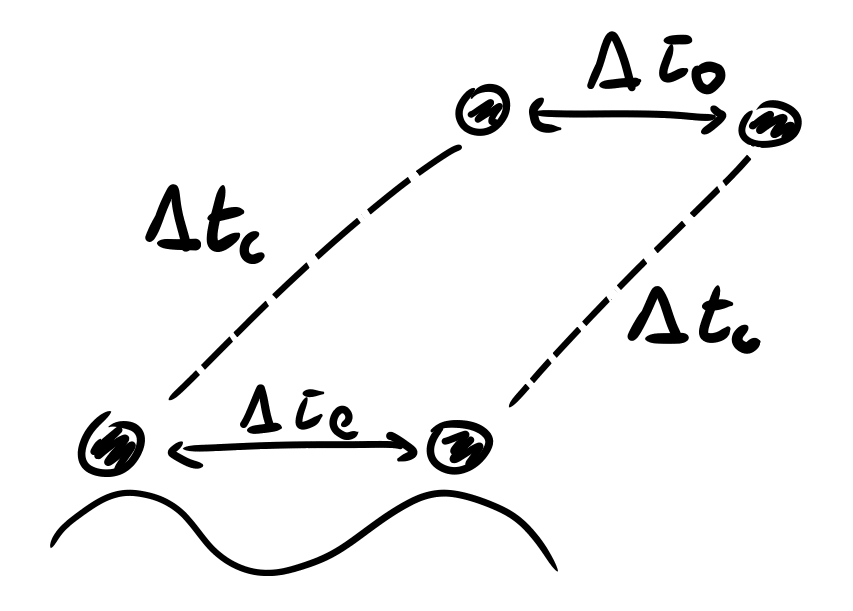
\includegraphics{michaelmas/gr/2018/11/20181109_redshift.png}
    \caption{The setup for our discussion of redshift. An emitter at $r=r_e$ sends out flashes of light at regular intervals of proper time $\Delta \tau_e$, which are received at some coordinate time $\Delta t_c$ later by an observer sitting out at $r=r_o$ and measured at intervals of $\Delta \tau_o$. The emitter and observer agree upon the difference in coordinate time between the flashes, but they (correctly) disagree on the difference in proper time.}
    \label{fig:gravitationalredshift}
\end{figure}

Suppose that $d\theta,d\phi=0$ so that our emitter and observer are only radially separated. Since $ds^2=0$ for null geodesics, the flashes of light from the emitter obey $dt^2=dr^2/V(r)^2$, so the light from a crest takes a coordinate time $\Delta t_c=\int_{r_e}^{r_o}dr/V(r)$ to reach the observer at $r_o$. Since this is the same $\Delta t_c$ for the first and second flash and depends only on $r_e,r_o$, it must be that both the emitter and the observer agree on the coordinate time between flashes, $\Delta t$.

However, for both our emitter sitting at $r_e$ and our observer out at $r_o$, they are both at constant $r$ ($dr=0$) and so $ds^2=-V(r) dt^2$, which means that
\begin{align*}
    \Delta \tau_e^2&=V(r_e)\Delta t^2\\
    \Delta \tau_o^2 &= V(r_o)\Delta t^2.
\end{align*}
That is, our emitter and observer will disagree on the amount of proper time corresponding to the same $\Delta t$ between crests. In particular, since the change in coordinate time $\Delta t$ is the same, it follows that $$\frac{\Delta \tau_e^2}{\Delta \tau_o^2}=\frac{V(r_e)}{V(r_o)}.$$
We find that
\begin{align*}
    \frac{\Delta \tau_e}{\Delta \tau_o}&=\sqrt{\frac{V(r_e)}{V(r_o)}}\\
    &=\sqrt{\frac{1-2M/r_e}{1-2M/r_o}}\\
    &\approx 1-\frac{M}{r_e}+\frac{M}{r_o}\\
    &\approx 1-\frac{M}{r_o r_e}(r_o-r_e),
\end{align*}
so the period of proper time between flashes measured by the observer is slightly greater than the period measured at the emitter. In the weak field limit where $M/r$ is small, $r_o>r_e \implies \Delta \tau_o/\Delta \tau_e > 1$. This is the gravitational redshift, and it was first found by Pound and Rebka in 1959 at Harvard.

But note that if $V(r_0)=0$ then the redshift becomes infinite, which might lead us to think something has gone terribly wrong. However, if $V(r)=0$ then the line element $ds^2$ is not well-defined, so all that's happened is that the coordinates have broken down. 

As it turns out, this is merely a coordinate singularity and not a curvature singularity. One can write down for instance the Riemann tensor and show that nothing bad to the curvature happens at $r\to 2M$, and moreover if we pass to a different set of coordinates, we can pass through the event horizon without issue.

There are many sets of coordinates that have been defined for black holes, but the one we'll introduce today is the Eddington-Finkelstein coordinates. They comprise the following:
\begin{itemize}
    \item Null coordinates: constant along light rays
    \item Retarded coordinates:\footnote{These coordinates seem to be bad at $r=2M$, but in fact they are just what we need to cross the event horizon safely.} $$u=t-r-2M \ln \frac{r-2M}{2M}$$
    \item Advanced coordinates: $$v=t+r+2M\ln \frac{r-2M}{2M}$$
\end{itemize}
Look in particular at the $v,r,\theta,\phi$ coordinates. We have
\begin{align*}
    dv &= dt+(2M\frac{1}{r-2M}+1)dr\\
    &= dt+\frac{r}{r-2m}dr\\
    &= dt+\frac{dr}{V(r)}
\end{align*}
and so the line element becomes
\begin{align*}
    ds^2&= -V(dv -\frac{dr}{V})^2+\frac{dr^2}{V}+r^2(d\theta^2 +\sin^2\theta d\phi^2)\\
    &=-Vdv^2 +2dvdr+r^2(d\theta^2 +\sin^2\theta d\phi^2).
\end{align*}

Our metric now has off diagonal terms, but this is no problem. It is still symmetric if we separate out $dvdr$ and $drdv$, and $\det g =-r^4\sin^2\theta \neq 0$ so we expect it to be invertible. Explicitly we can write it as
$$
g_{ab}=\begin{pmatrix}
    -V & 1 & 0 & 0\\
    1 & 0 & 0 & 0\\
    0&0&r^2&0\\
    0&0&0&r^2\sin^2\theta
\end{pmatrix}.
$$
Moreover the inverse is perfectly well-defined away from $r=0$,\footnote{It might seem like there's also an issue with $\theta=0$, but this is just the regular coordinate badness of spherical polar coordinates. Remember that $\phi$ becomes ill-defined at the north pole, $\theta=0$, even though the north pole is otherwise totally unremarkable as a point on the sphere. This is nothing more than the garden-variety coordinate singularity of generic spherical coordinates.}
$$
g^{ab}=\begin{pmatrix}
    0 & 1 & 0 & 0\\
    1 & V & 0 & 0\\
    0 & 0 & 1/r^2 &0\\
    0 & 0 & 0 & 1/(r^2\sin^2\theta)
\end{pmatrix}.
$$
In particular nothing blows up at $r=2M$, so it seems that we've constructed equally good coordinates to sail past the coordinate singularity at the event horizon.

If we take $v,\theta,\phi$ constant, then $ds^2=0$, so lines of constant $v$ are null lines. ($r$ can of course still change.) One such line has $v=0,r=2M$ (the event horizon itself) and what we discover is that as we pass the event horizon, the light cone has tipped over and any timelike trajectory must be directed towards decreasing $r$. That is, beyond the event horizon ($r<2M$) one can no more escape the gravitational pull of a black hole than one can escape the inexorable march of time(like trajectories).
%insert picture

Curiously, a photon on the surface $V=0$ ($r=2M$) can simply stay there in a stable circular orbit. We call $V=0$ the event horizon, and it is also (by our earlier calculation) a surface of infinite redshift. This is why we call it a black hole-- not only can light not escape, but any light from an infalling emitter will be increasingly redshifted as the emitter approaches the event horizon. If one throws a flashing light clock (i.e. with constant period in its own proper time) into the black hole, an observer sitting far away from the black hole at constant $r$ will see the flashes become increasingly separated, but they will never actually stop.\footnote{It's a bizarre fact that the clock can cross the event horizon in finite time, but due to the redshift, an external observer can never actually see it fall in. Stranger yet is the viewpoint of the infalling observer, who notices nothing unusual with regards to curvature as they pass the event horizon, but looking radially out will see the light from the outside world increasingly blueshifted. As your light cone tips over, you would see the entire future of the universe outside the black hole, but you would never be able to tell anyone what you saw.}

There is a ``hoop conjecture'' widely attributed to Thorne\footnote{Professor Perry mentioned Yau and collaborators contributing to this work, but I was unable to find any sources which substantiated this claim.} which states that if the amount of matter (with a total mass $M$) is confined to a proper distance $l\leq 2M$, then an event horizon will form. The details of this conjecture and attempts to prove it are beyond the scope of this class, so we'll just state it without proof and hope it sounds reasonable.

As a final note for today, there is still one problem with the black hole-- just look at the curvature as a function of $r$. For instance, if we calculate the trace over all components of the Riemann tensor, we see that
$$R_{abcd}R^{abcd}\sim M^2/r^6$$ up to some numerical factors, and as $r\to 0$, $R_{abcd} R^{abcd}\to \infty$ diverges. In electrodynamics we might say that a divergence is simply unphysical because of quantum effects, but there's no sensible theory of quantum gravity that will let us make sense of this yet in a gravitational context. In classical physics we know what to do-- just call the singularity a boundary of spacetime. But it ought to be rather disturbing that one could simply sail not only over the event horizon but over the boundary of spacetime into... where, exactly? This is a major problem for classical (and quantum) gravity and there is no good solution. Yet.\footnote{``That's what I can tell you about singularities. They're there.'' --Malcolm Perry}

\subsection*{Non-lectured aside: cosmic censorship} Here's a little reflection related to Prof. Jorge Santos's essay this year! A priori, point singularities are maybe not so disturbing to us, since they have no spatial extent and you might think a physical observer could never actually cross it. Fair enough. But in spinning (Kerr) and charged (Reissner-Nordstr\"om) black holes, we get entire singular surfaces called Cauchy horizons. Now we could imagine going right through a Cauchy horizon in finite proper time (I haven't proved this, but one can write down the geodesics and show it's true), and beyond the Cauchy horizon, the Einstein equations fail to predict our trajectory based on the past. Determinism breaks down. 

Some physicists (most notably Roger Penrose) have therefore proposed the \term{strong cosmic censorship conjecture}, which suggests (in one phrasing) that Cauchy horizons do not represent physically realizable solutions to the Einstein equations.\footnote{There's also the \term{weak cosmic censorship conjecture} which says roughly that nature always conspires to hide away singularities behind event horizons. The two conjectures are related in spirit but formally distinct.} For instance, it might be that small perturbations (e.g. what are called quasinormal modes) to the event horizon set the black hole ringing like a bell, and this ringing behavior collapses and destroys the Cauchy horizon. Equivalently, if you read my footnote on blueshift earlier (following the discussion of the redshift near the event horizon), you might reason that from the perspective of any infalling observer, all the light from the entire lifetime of the external universe is blueshifted to infinitely high frequency and the energy of this light simply obliterates any poor soul with aspirations of sailing off the edge of spacetime. Cosmic censorship is saved.

Or is it? Recent work by \href{https://news.berkeley.edu/2018/02/20/some-black-holes-erase-your-past/}{Peter Hintz of MIT and others} suggests that there's a loophole in certain kinds of spacetimes. In particular, our solutions assumed asymptotically flat boundary conditions. This is what allows the light from eternity to send our hapless observer to the Shadow Realm. However, if our black hole sits in a positively curved, expanding spacetime (asymptotically de Sitter, not to be confused with anti-de Sitter, AdS), then the blueshift is suppressed by the expansion of spacetime. This is particularly relevant because our universe seems to have a small but non-negligible positive cosmological constant, and therefore looks to be asymptotically de Sitter. Under certain conditions, this suppression is enough to overcome the infinite blowup normally associated with the blueshift. Our observer seems to have gotten a reprieve, at the cost of strong cosmic censorship. Is there another physical argument we've missed which closes this loophole, or is cosmic censorship in real trouble? This is an open research question and the topic of my Part III essay this year.

For additional reading, see Harvey Reall's review \href{https://physics.aps.org/articles/v11/6}{here} as well as the recommended readings for the essay:
\begin{itemize}
    \item V. Cardoso, J. L. Costa, K. Destounis, P. Hintz and A. Jansen, ``Quasinormal modes and Strong Cosmic Censorship,'' Phys. Rev. Lett. \textbf{120}, no. 3, 031103 (2018), \url{https://doi.org/10.1103/PhysRevLett.120.031103}
    \item O. J. C. Dias, H. S. Reall and J. E. Santos, “Strong cosmic censorship: taking the rough with the smooth,” JHEP \textbf{1810}, 001 (2018), \url{https://doi.org/10.1007/JHEP10(2018)001}.
\end{itemize}

    
\section{Monday, November 12, 2018}
    Last time, we wrote down the metric for a black hole in Eddington-Finkelstein coordinates. It takes the form
$$ds^2=-\left(1-\frac{2M}{r}\right) dv+2dvdr+r^2 (d\theta^2+\sin^2 \theta d\phi^2).$$

We found that $v$ is finite on the horizon, so the singularity at $r=2M$ was simply a coordinate singularity. However, the singularity at $r=0$ is a much bigger problem. We found that the trace of the Riemann tensor (and therefore the Weyl tensor, since this is a vacuum spacetime) diverges badly as $r\to 0$:
$$R_{abcd}R^{abcd}=C_{abcd}C^{abcd}\sim m^2/r^6.$$

One might think that in assuming spherical symmetry we've added some extra assumption to produce this singularity, but in fact Penrose showed under a set of more general conditions that if there is a horizon, then there must be a singularity.\footnote{This is Penrose's 1965 singularity theorem. The converse is not proven yet (singularity $\implies$ horizon) and is the statement of the weak cosmic censorship conjecture, also due to Penrose.}

Moreover, black holes (unlike diamonds) are not forever.\footnote{Technically diamonds are also metastable states of carbon, so make of that what you will.} In 1974, Hawking found that when particle-antiparticle pairs are produced very near to the event horizon (as vacuum fluctuations), one of the two may fall into the black hole while the other escapes. The result is that the black hole behaves like a thermally radiating black body of temperature $1/8\pi M=T_{\text{Hawking}}$. In units, $T_{\text{Hawking}}=6\times 10^{-8}\left(\frac{M_S}{M}\right)$ Kelvin, where $M_S$ is the solar mass of $2\times 10^{33}$ grams.

However, thermal radiation is associated to an energy flux of $\sigma T^4\times$ surace area, where $\sigma$ is the Stefan-Boltzmann constant. One expects that a black hole will generically radiate not just photons but all elementary particles. However, rewriting the mass-temperature reation as $M=1/8\pi T$ and interpreting the mass $M$ as an energy, we find that the specific heat is
$$C=\P{M}{T}=-\frac{1}{8\pi T^2}<0.$$
The fact that the specific heat is negative implies that the black holes are unstable.

If we then compute $dM/dt$, we find that
$$\frac{dM}{dt}=-(\text{energy flux})\sim -\frac{1}{M^4}M^2,$$
which means that a black hole has a lifetime scaling as $M^3$, and given enough time, a black hole will evaporate. For astrophysical black holes, this takes place on a timescale of about $10^{67}(M^2/M_S^2)$ years.

However, black hole evaporation is important for the theory of black holes-- for instance, it's not totally clear what happens to the singularity when a black hole evaporates. What happened to the information (about the electron states, molecular configurations, etc.) contained in all the stuff that fell in? This is related to the black hole information paradox, which we will likely see more about in the \emph{Black Holes} course in Lent.

Let us also note that black holes generically form when when an amount of matter $M$ is confined to some distance of scale $R\sim 2M$. However, the laws of physics (as far as we are concerned here) are invariant under time reversal, so where we defined our retarded coordinate
$$v=t+r+2m\ln (\frac{r-2M}{2M}),$$
we could just as easily flip the sign on $t$ to get the advanced coordinate
$$u=t-r-2M(\ln \frac{r-2M}{2M}).$$

In the $(u,r,\theta,\phi)$ coordinates the metric now takes the form 
$$ds^2=-(1-2M/r)du^2-2dudr +r^2(d\theta^2 +\sin^2\theta d\phi^2).$$
We find that all timelike lines must leave the horizon, so this is essentially the time-reversed version of a black hole, usually called a white hole.

In practice, white holes do not appear to exist in nature. Solutions of the wave equation in electrodynamics,
$$\Box A^a=-\mu_0 j^a,$$
one picks the retarded solutions and not the advanced solutions in order to preserve some nice idea of causality.\footnote{Wonder if there's a meaningful concept of thermodynamics for white holes.}

And now for something completely different. We'll dip into cosmology in a GR context for a minute. Much of the seminal work here is associated to Lema\^itre (1972, Belgium), Friedmann (1922, Russia), Robertson (1931, US), and Walker (1937, UK). Between them, they developed models of the entire universe beginning from the assumptions that space is homogeneous (the same everywhere) and isotropic (the same in every direction). These are enough to suggest that the spatial part of our metric ought to describe a maximally symmetric space with a full set of six Killing vectors for a 3-dimensional space. Indeed, the simplest possibility is just flat $\RR^3$,
$$d\sigma^2=dr^2+r^2(d\theta^2+\sin^2\theta d\phi^2).$$
We call this $k=1$, and its symmetries are simply those of Euclidean 3-dimensional space. However, we could also consider the geometry of $S^3$ in hyperspherical coordinates,
$$d\sigma^2=dr^2+\sin^2 r(d\theta^2+\sin^2\theta d\phi^2).$$ Here, $r$ and $\theta$ run from $0\leq r,\theta\leq \pi$ and $\phi$ runs from $0\leq \phi < 2\pi$. The symmetry group is $SO(4)$, and we say this has $k=1$. However, note that unlike in $\RR^3$, space is of finite spatial extent here. If we denote the metric by $\gamma_{ij}$ with $i,j=1,2,3$, we have
$$R_{ijkl}=\frac{1}{6}R(\gamma_{ik}\gamma_{jk}-\gamma_{il}\gamma_{jk}),$$
where $R$ is the Ricci scalar, and the Ricci scalar is now identified with the scalar curvature from regular differential geometry. (This is a bit like de Sitter space.)

Lastly, we can take $k=-1$, the hyperboloid with metric $$d\sigma^2=dr^2+\sinh^2 r (d\theta^2 +\sin^2\theta d\phi^2).$$
Here, the coordinate ranges are $0\leq r < \infty, 0\leq \theta \leq \pi, 0\leq \phi < 2\pi.$ Now ,we get a similar Riemann tensor
$$R_{ijkl}=\frac{1}{6}R(\gamma_{ik}\gamma_{jk}-\gamma_{il}\gamma_{jk})$$
but with $R<0.$

\begin{defn}
More generally, let us now take the spacetime metric in $3+1$ dimensions to be
$$ds^2=-dt^2+a^2(t) d\sigma_k^2$$
where $k=0,\pm 1$ and $a(t)$ is some cosmological scale factor which depends on time. That is, the metric separates into a time component and a spatial component whose only dependence on $t$ is through the scale factor $a(t)$. Such metrics are known as \term{FLRW spacetimes} (for Friedman, Lema\^itre, Robetrson, and Walker).\footnote{You'll also hear FRW, RW, and FL used to describe such metrics. It depends on who you want to give the credit to.}
\end{defn}

Now, there should be an energy-momentum tensor describing all the stuff in the universe, since our universe is certainly not a vacuum solution. There's stuff like galaxies and dark matter (about $26$\%), dark energy (about $74$\%), and radiation (not much). We might write the energy-momentum tensor in the following form:
$$T_{ab}=(p+\rho)u_a u_b +p g_{ab},$$
where $u^a$ is a velocity four-vector, $\rho$ is the energy density, and $p$ is the pressure.

We'll now state some facts about the equations of state for various sorts of energy content. Galaxies and dark matter are free and don't interact much, so for them we have $p=0$, sometimes called \term{dust}. On the other hand, radiation (in particular thermal radiation) obeys an equation of state $p=\frac{1}{3}\rho$. Finally, dark energy (which remains largely mysterous) has an equation of state thought to be $p=-\rho$ with $\rho>0$.

Let's look at the energy-momentum tensor for dark energy for a second. The velocity term is zero by the equation of state ($p+\rho=0$), so
$$T_{ab}=-\rho g_{ab}.$$
Of course, this is totally equivalent to adding a term $\Lambda g_{ab}$ in the Einstein equations, so one can trade dark energy for a cosmological constant $\Lambda=8\pi \rho_{DE}$ with $\rho_{DE}$ the energy density of the dark energy.

What about all the regular massive stuff? Suppose we assume that on average, galaxies have no intrinsic motion of their own, so they can be put into a rest frame, $u^a=(1,0,0,0)$ (normalized by $u^a u_a=-1$). Of course, the whole point of the energy-momentum tensor is that it is conserved,
$$\nabla_a T^{ab}=0,$$
so writing this out explicitly we find that
$$\nabla_a((p+\rho)u^a u^b + p g^{ab})=0.$$
In the rest frame, $b=0$ is the only equation with any content, so considering $p,\rho,a$ as all functions of $t$ we find that
$$\dot \rho=-3(\dot p+\rho)\dot a/a,$$
where $\cdot=d/dt$, a derivative with respect to coordinate time. Now if $p=0$ then
$$\dot \rho =3\rho \dot a/a \implies \rho(t)=\rho_0 a_0^3/a^3(t).$$
Imagine measuring $\rho$ now, corresponding to a time $t_0$ when the universe has some scale factor $a_0$. This looks like the equation for the conservation of mass.
    
\section{Wednesday, November 14, 2018}
    Last time, we wrote down the equation relating the scale factor $a$ to the content of spacetime:
$$\dot \rho = -3(p+\rho)\dot a/a.$$

Some examples of the stuff in spacetime include dust ($p=0,\rho_M=\rho_0 a_0^3/a^3$), radiation ($p=\rho/3$, with $\rho_{rad}=\rho_0 a_0^4/a^4$, and dark energy ($p=-\rho$, $\rho_\Lambda=$constant).
But what we observe is that in an expanding universe, radiation is thus diluted faster ($a^{-4}$) than matter ($a^{-3}$), which is diluted faster than dark energy.

Now recall that we have written the Einstein equations
$$R_{ab}-\frac{1}{2}R g_{ab}+\Lambda g_{ba}=8\pi T_{ab},$$
where we have supposed the metric separates into a time component and a scaled spatial component,
$$ds^2=-dt^2+a^2(t) d\sigma^2.$$
Now using the form of $T_{ab}$ in terms of $\rho,p$, we get
$$4\pi(\rho+3p)-\Lambda=-3\ddot a/a,$$
which can be written as
$$3\dot a^2=8\pi \rho a^2 +\Lambda a^2 -3k.$$
This is sometimes known as the Raychaudhuri equation or the energy equation.%where does this come from? Check Sean Carroll later

In the absence of matter, there is just $\Lambda$ to govern the curvature and expansion. $\Lambda >0$ gives de Sitter space, $\Lambda=0$ Minkowski space, and $\Lambda <0$ anti de Sitter space. What happens if we put some matter in?

If we now take dust with $p=0$ and start with a $\Lambda=0,k=0$ universe, we get
$$a(t)\sim t^{2/3},$$
a power law. Suppose we take boundary conditions $a(t_0)=a_0.$ Then
$$a(t)=a_0 (t/t_0)^{2/3},$$
and we can relate the density to time,
$$\rho_0=\frac{1}{6\pi t_0^2}.$$
That is, we can relate $\rho_0$ the density at $t_0$ to the age of the universe. But notice that as we rewind to $t=0$, the curvature (or equivalently the density) blows up-- spacetime becomes singular. This turns out to be fairly generic behavior in the absence of a cosmological constant. Theorems of Hawking and Penrose in fact guarantee that in an expanding universe with ordinary matter ($\Lambda=0$), there must be an initial singularity. %maybe add a link here later
Like most singularities, there is really nothing more we can say about it.

Let's now consider the $k=1$ case, still for dust ($\Lambda=0,p=0$). The Raychaudhuri equation now gives us
$$\dot a=\sqrt{\frac{8\pi \rho_0 a_0^3}{3a}-k}.$$ If we now make the substitution $a=\frac{8\pi \rho_0 a_0^3}{3}\sin^2\theta$, the equation becomes
$$\frac{16\pi \rho_0 a_0^3}{3} \int \sin^2\theta d\theta =t,$$
which has the solution
$$\frac{8\pi \rho_0 a_0^3}{3}(\theta-\frac{1}{2}\sin 2\theta)=t.$$ Thus
$$a(t)=\frac{8\pi \rho_0 a_0^3}{3}\sin^2\theta,$$
which is the formula for a cycloid. The universe therefore expands out to some maximum scale at $\theta=\pi/2$, and then contracts back to a singularity at $t=\pi$.

What if $k=-1$? Then we ought to modify the sine to a sinh, $$a=\frac{8\pi\rho_0 a_0^3}{3}\sinh^2 \theta.$$
The solution is now
$$t=\frac{9\pi\rho_0 a_0^3}{3}(\frac{1}{2}\sinh 2\theta -\theta),$$
which leads to continuous expansion. It is at first independent of $k$: for small $t$,
$$a(t)\sim t^{2/3}.$$
But at late times, $k=-1$ looks like linear expansion.

What we find is that it is hard to measure $k$ when $t$ is small-- at early times, all expansions look pretty similar in their scaling-- see Fig. \ref{fig:flrw_metric}.

\begin{figure}
    \centering
    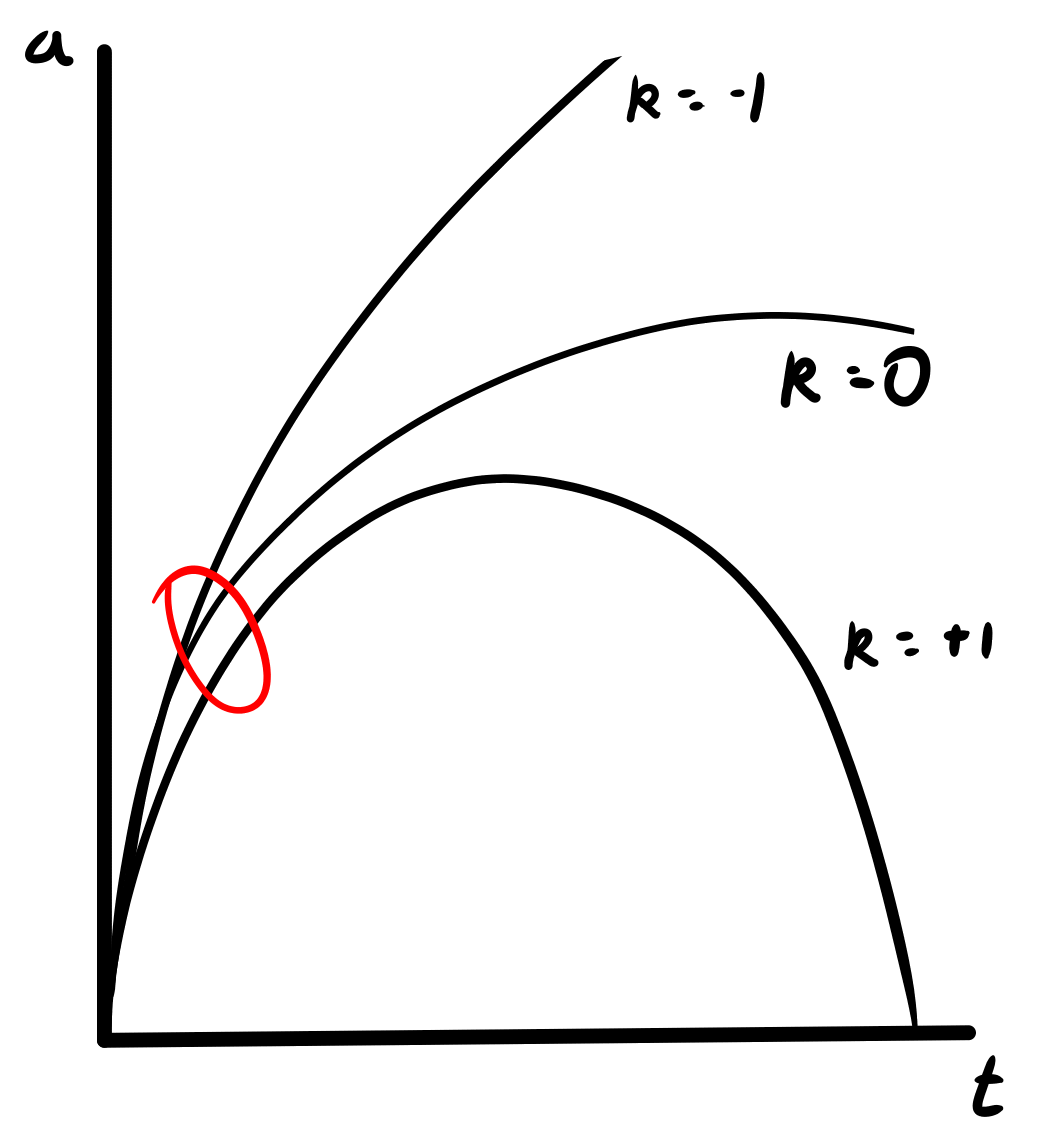
\includegraphics{2018/11/20181114_scalefactor.png}
    \caption{The scale factor as a function of time. We have written the metric as $ds^2=-dt^2 +a^2(t) d\sigma_k^2$, where $d\sigma_k^2$ is a purely spatial metric. The spatial part can be positively curved ($k=+1$), negatively curved ($k=-1$), or flat ($k=0$). At early times (the circled red region), all three scenarios expand similarly, but the $k=+1$ solution eventually contracts back to a singularity, while the $k=0$ and $k=-1$ solutions expand forever. Experimentally, we cannot yet distinguish between which of these scenarios describes our universe.}
    \label{fig:flrw_metric}
\end{figure}

\subsection*{Gravitational radiation} Just as Maxwell's equations in vacuum have plane wave solutions, we expect that Einstein's equations in vacuum might also reasonably have some wave solutions. We can treat these solutions using perturbation theory. Think about small perturbations to the metric,
$$g_{ab}=g_{ab}^{(0)}+h_{ab},$$
and let's work in linear order in $h$.

Then we can expand the Einstein equations accordingly. For instance,
$$\delta R_{ab}=-\frac{1}{2}\Box h_{ab}+\frac{1}{2}\nabla_d \nabla_a h^d_b +\frac{1}{2}\nabla_d \nabla_b h^d_a -\frac{1}{2}\nabla_a \nabla_b h,$$
with $h=h_{ab}{g^{(0)}}^{ab}$. Note that the covariant derivatives $\nabla$ are taken with respect to the original unperturbed metric $g^{(0)}$. The variation of the Einstein equations is therefore
$$\delta R_{ab}-\frac{1}{2}\delta R g_{ab}^{(0)} -\frac{1}{2}R h_{ab}=8\pi T_{ab}.$$
 Here, we think of $T_{ab}$ as the source of gravitational radiation, so $T_{ab}$ is of order $h$.

To simplify somewhat, we take $g^{(0)}$ to be Minkowski space and work in $t,x,y,z$ coordinates. Thus $\nabla_a$ becomes a partial derivative and $\Box$ is just the flat space wave operator. Our equations simplify to
$$-\Box h_{ab}+\p_d \p_a h^d_b +\p_d \p_b h^b_a -\p_a \p_b h=16\pi T_{ab},$$
which is the analog of Maxwell's equation-- written in terms of a vector potential, that looks like
$$\Box A^a -\p_b \p^a A^b=-\mu_0 j^a.$$
It is often convenient to solve Maxwell's equations with an appropriate choice of gauge. Let us try to find something equivalent for our Einstein equations.

Suppose one makes a coordinate transformation
$$x^a \mapsto {x'}^a = x^a +\epsilon^a.$$
We previously found that if the line element is invariant, this changes the metric by $\nabla_a \epsilon_b +\nabla_b \epsilon_a$. When such transformations were isometries (leave the metric unchanged), these $\epsilon$s just solved Killing's equation. In our problem, this changes the metric by
$$\p_a \epsilon_b +\p_b \epsilon_a.$$

Thus $h'_{ab}=h_{ab}+\p_a \epsilon_b +\p_b \epsilon_a$ represents the same physical perturbation, and we shall choose $h'_{ab}$ to obey
$$\p_a({h'}^{ab}-\frac{1}{2}\eta^{ab}h')=0,$$
which we call the \term{harmonic gauge}. This is analogous to setting $\p_a A^a =0$ in electrodynamics.

Can we always do this? If we expand out this expression, we find that
$$0=\p_a({h'}^{ab}-\frac{1}{2}\eta^{ab}h')=\p_a(h^{ab}-\frac{1}{2}\eta^{ab}h)+\p_a \p^a \epsilon^b +\p_a \p^b \epsilon^a -\frac{1}{2} \eta^{ab} \p_a \underbrace{(2\p_c \epsilon^c)}_{h'}.$$
These last two terms cancel, so setting this gauge is equivalent to solving
$$\Box \epsilon^b = -C^b$$ for
$C^b=\p_a(h^{ab}-\frac{1}{2}\eta^{ab}h).$
But we can always solve this equation by constructing a Green's function for $\Box$, so one can always choose this gauge. We'll show this explicitly in the next lecture.

\subsection*{The Green's function for $\Box$} Generically, our equation takes the form
$$-\frac{\p^2 \epsilon^b}{\p t^2}+\nabla^2 \epsilon^b =-C^b.$$
Here, $\epsilon^b, C^b$ are functions of $\vec x,t$. Let us take the Fourier transform and write in $\vec p,\omega$ variables as
$$\hat \epsilon(\vec p,\omega)=\int d^3x dt \epsilon(\vec x,t) e^{-i\omega t +i\vec p \cdot x}.$$
Time derivatives bring down $\omega$s and $\nabla$s bring down $\vec p$,s so our equation in Fourier space reduces to
$$(\omega^2-\vec p^2) \hat \epsilon(\vec p, \omega)=-\hat C(\vec p, \omega).$$
Thus we rewrite
$$\hat \epsilon(\vec p, \omega)=-\frac{\hat C(\vec p,\omega)}{\omega^2-\vec p^2}.$$
We need only take the inverse Fourier transform to get us back to real space.
\end{document}